\documentclass[11pt]{ainotes}

\title{Cognition and Neuroscience\\(Module 1)}
\date{2023 -- 2024}
\def\lastupdate{{PLACEHOLDER-LAST-UPDATE}}

\DeclareAcronym{psp}{short=PSP, long=postsynaptic potential, long-plural=s}
\DeclareAcronym{epsp}{short=EPSP, long=excitatory postsynaptic potential, long-plural=s}
\DeclareAcronym{ipsp}{short=IPSP, long=inhibitory postsynaptic potential, long-plural=s}
\DeclareAcronym{ap}{short=AP, long=action potential, long-plural=s}
\DeclareAcronym{cns}{short=CNS, long=central nervous system}
\DeclareAcronym{pns}{short=PNS, long=peripheral nervous system}
\DeclareAcronym{rl}{short=RL, long=reinforcement learning}
\DeclareAcronym{nr}{short=NR, long=no response}
\DeclareAcronym{us}{short=US, long=unconditioned stimulus}
\DeclareAcronym{ur}{short=UR, long=unconditioned response}
\DeclareAcronym{cs}{short=CS, long=conditioned stimulus}
\DeclareAcronym{cr}{short=CR, long=conditioned response}

\newtheorem*{casestudy}{Case study}

\begin{document}
    
    \makenotesfront
    \printacronyms
    \newpage

    \chapter{Introduction}



\section{Definitions}

\begin{description}
    \item[Neuroscience] \marginnote{Neuroscience}
        Study of the nervous system (structure aspects) on various levels of detail:
        \begin{descriptionlist}
            \item[Molecular] Proteins and molecular signaling of the nervous system.
            \item[Cellular] Morphological and physiological properties of neurons.
            \item[Neural system] Creation and functioning of networks of neurons.
        \end{descriptionlist}


    \item[Cognition] \marginnote{Cognition}
        Mental processes (function aspects) that react to inputs. 
        It involves processes regarding the acquisition, storage, manipulation, and retrieval of information.
        \begin{descriptionlist}
            \item[Perception] Information from the environment.
            \item[Attention] Focus on a specific stimulus in the environment.
            \item[Learning] Merging new information with prior knowledge.
            \item[Memory] Encoding, storing, and retrieving information.
            \item[Action] Interact with the environment using perceived information.
            \item[Language] Understanding and producing spoken or written thoughts.
            \item[Higher reasoning] Decision-making and problem-solving.
        \end{descriptionlist}


    \item[Biomimicry] \marginnote{Biomimicry}
        Solving problems by taking inspiration from elements of nature.

        As proof of general intelligence\footnote{
\includegraphics[width=1cm]{img/doubt.png}}, 
        the human brain is taken as the model for artificial intelligence.
        Moreover, a successful brain-inspired AI application can 
        provide a possibly plausible explanation of the functioning of the brain.
        
        However, a brain differs from a computer in many aspects:
        \begin{itemize}
            \item Hardware and software are distinct while mind and brain are not.
            \item Machines learn by exploiting the capability of using a large memory
                while brains have limited capacity but high generalization ability.
            \item Brains produce both electrical and biochemical signals and 
                have feedforward, feedback, and recurrent connections
                while machines typically only employ feedforward connections.
        \end{itemize}

        \begin{description}
            \item[Structure emulation] 
                Mimic or reverse engineer the structure of the brain (e.g. Blue Brain Project).

            \item[Function emulation] 
                Mimic a neural system on the algorithmic level (e.g. Deep Mind).
        \end{description}


    \item[Cognitive neuroscience] \marginnote{Cognitive neuroscience}
        Study of the relationship between the physical brain and the intangible mind (thoughts, ideas).
        In other words, it studies the relationship between structure and function.

        \begin{example}[Severed Corpus Callosum\footnote{\url{https://www.youtube.com/watch?v=lfGwsAdS9Dc}}]
            Normally, the right and left hemispheres of the brain can communicate. 
            Moreover, the left visual field is sent to the right hemisphere and 
            the right visual field is sent to the left hemisphere.

            In patients where the hemispheres are split, a text shown on the right visual side is recognized as 
            the speech capabilities are located in the left hemisphere,
            while a text shown on the left visual side does not trigger any speech reaction.
        \end{example}
\end{description}



\section{Neuroscience history}

Two main schools of thought emerged and are still the subject of ongoing debates:
\begin{descriptionlist}
    \item[Localizationism] \marginnote{Localizationism}
        Specific regions of the brain are responsible for particular faculties.

        Assuming localizationism, 52 distinct regions with different neurons can be identified.

    \item[Aggregate field theory] \marginnote{Aggregate field theory}
        The brain works as a whole for mental functions.
\end{descriptionlist}


\subsection{Neuron doctrine}
\marginnote{Neuron doctrine}
The nervous system is made of a discrete amount of individual neurons (and not a continuous tissue).

\begin{description}
    \item[Principle of dynamic polarization] 
        Electrical signals in a neuron flow only in a single direction.

    \item[Principle of connectional specificity] 
        Neurons do not connect randomly but make specific connections at particular contact points.

    \item[Synapse] \marginnote{Synapse}
        Point of contact of two neurons. A synapse can be chemical or electrical.
\end{description}



\section{Cognitive science history}

\begin{description}
    \item[Rationalism] \marginnote{Rationalism}
        All knowledge can be derived through reasoning, without sensory experiences.

    \item[Empiricism] \marginnote{Empiricism}
        The brain starts as a blank slate and knowledge is added through sensory experiences.

    \item[Associationism] \marginnote{Associationism}
        Inspired by empiricism.
        Learning happens by correlating individual experiences (e.g. actions followed by a reward will be repeated).

    \item[Behaviorism] \marginnote{Behaviorism}
        Inspired by empiricism. 
        Everyone has the same neural basis that is improved through learning.
        Learning only involves observable behaviors.
\end{description}

\begin{remark}
    Associationism and behaviorism are not able to explain all types of learning (e.g. language).
\end{remark}

\begin{description}
    \item[Cognitivism] \marginnote{Cognitivism}
        The psychological and biological levels of an individual cannot be separated.
        Learning is based on the biology of the neurons.
\end{description}
    \chapter{Nervous system anatomy and physiology}


\begin{description}
    \item[Central nervous system] Brain and spinal cord.
    \item[Peripheral nervous system] Nerves that branch off from the brain and the spine.
\end{description}

\section{Individual cells}

% A nervous system has two types of cells:
% \begin{descriptionlist}
%     \item[Neurons/nerve cells] 
%     \item[Glia cells/neuroglia] 
% \end{descriptionlist}


\subsection{Glia cells / Neuroglia}
\marginnote{Glia cells/Neuroglia}
Cells that support neurons.
There are 2 to 10 times more glia cells than neurons.\\

\begin{minipage}{0.89\textwidth}
    \begin{descriptionlist}
        \item[Microglia] \marginnote{Microglia}
            Immune system cells located in the central nervous system.
            They intervene in response to toxic agents or to clear dead cells.
            \begin{itemize}
                \item Responsible for antigen presentation (determine the type of external agent).
                \item Become phagocytes (cells that ingest harmful agents) during injuries, infections, or degenerative diseases.
            \end{itemize}
    
            \begin{remark}
                In patients affected by Alzheimer's disease, microglia may become hyperactive and damage neurons.
            \end{remark}
    \end{descriptionlist}
\end{minipage}
\begin{minipage}{0.1\textwidth}
    \centering
    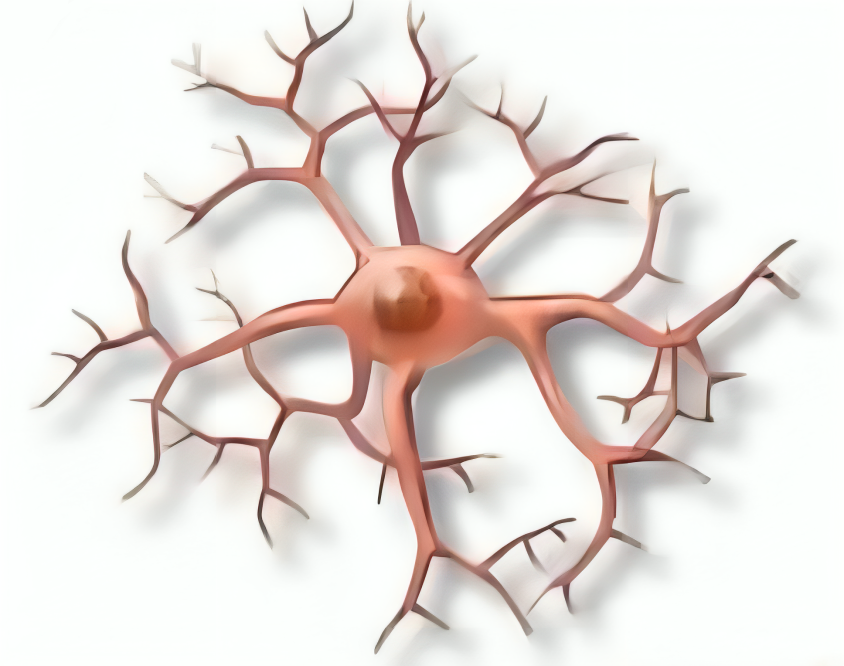
\includegraphics[width=\textwidth]{./img/microglia.png}
\end{minipage}\\[1em]

\begin{minipage}{0.79\textwidth}
    \begin{descriptionlist}
        \item[Astrocytes] \marginnote{Astrocytes}
            Star-shaped cells located in the central nervous system.
            They surround neurons and are in contact with the brain's vasculature.
            \begin{itemize}
                \item Provide nourishment to neurons.
                \item Regulate the concentration of ions and neurotransmitters in the extracellular space.
                \item Communicate with the neurons to modulate synaptic signaling.
                \item Maintain the blood-brain barrier that separates the tissues of the central nervous system and the blood.
            \end{itemize}
    \end{descriptionlist}
\end{minipage}
\begin{minipage}{0.2\textwidth}
    \centering
    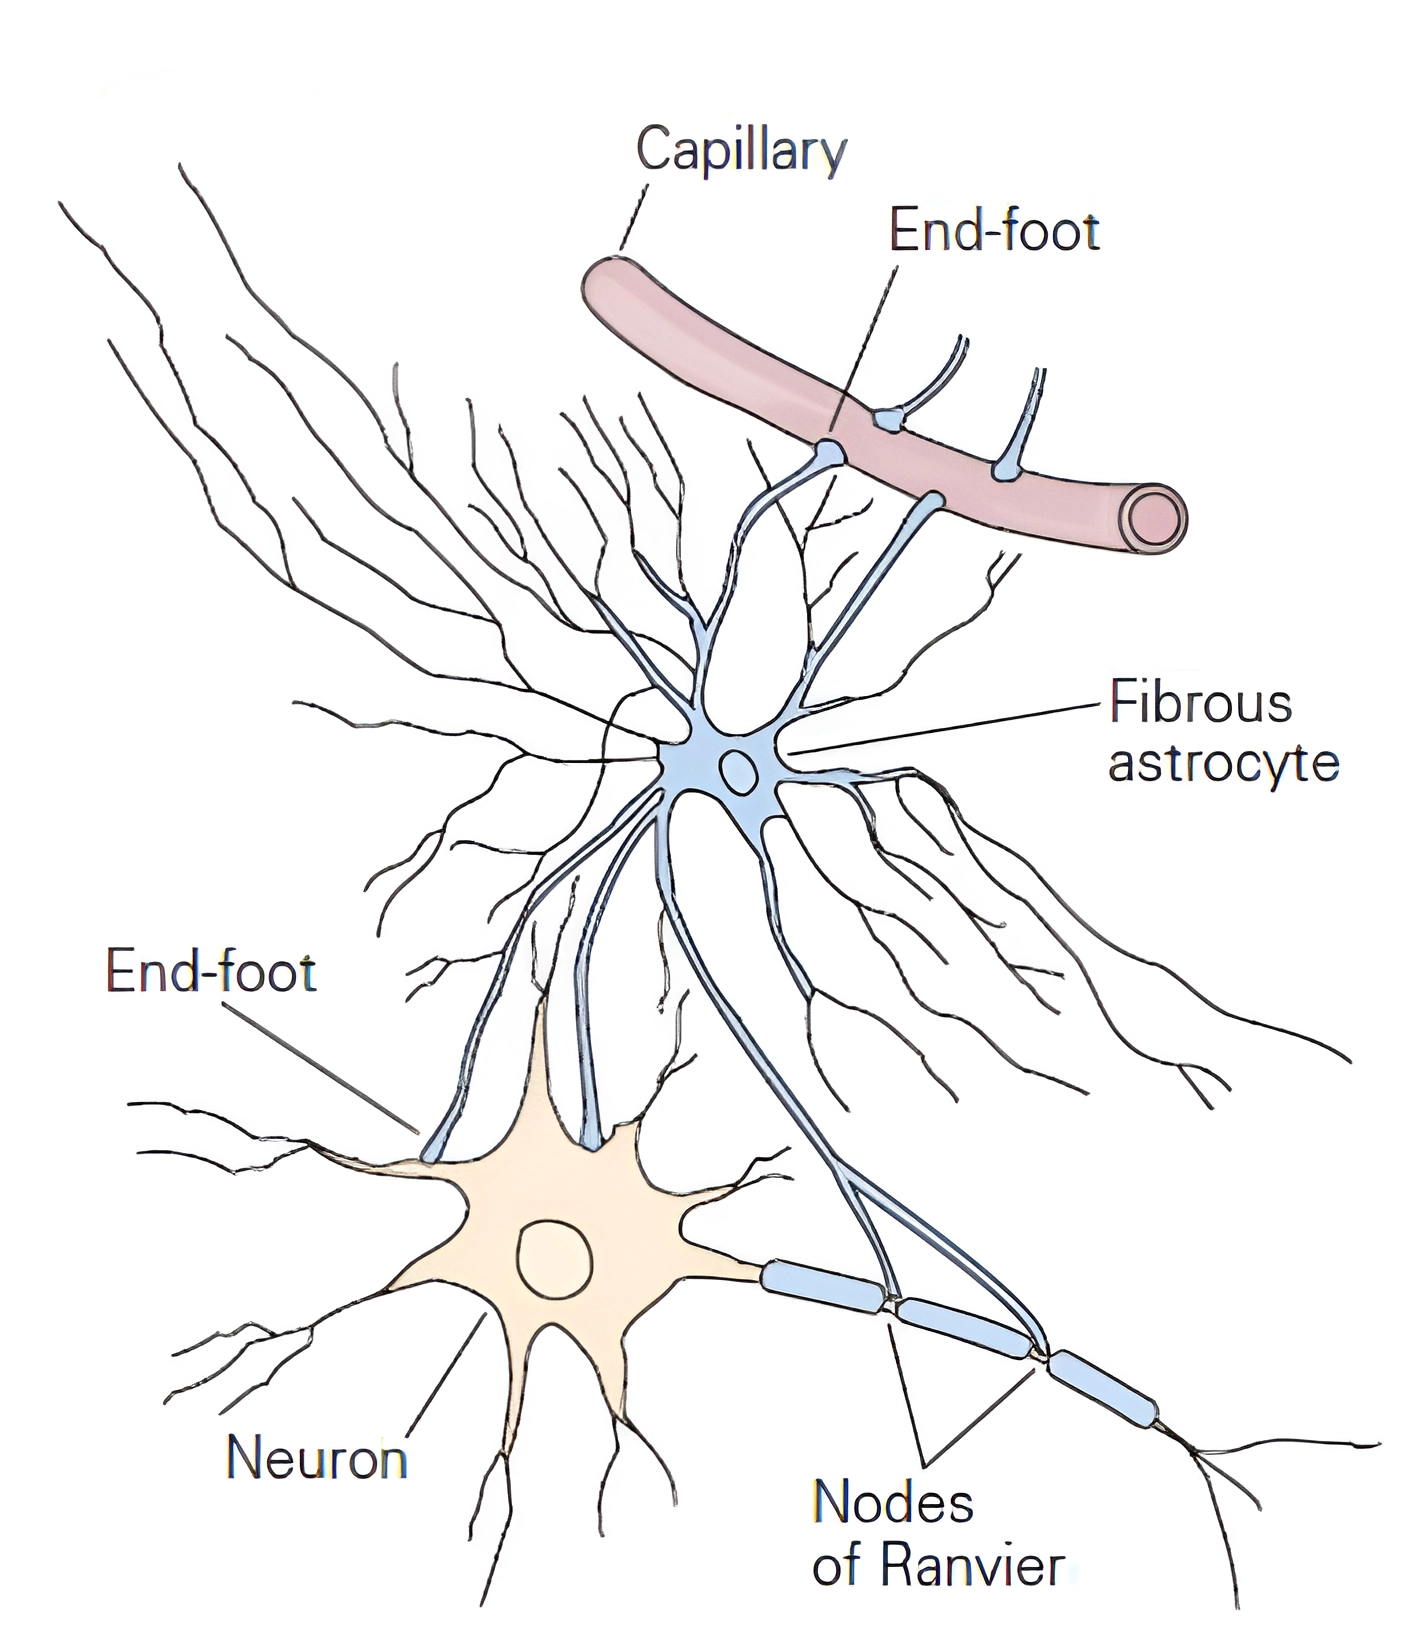
\includegraphics[width=\textwidth]{./img/astrocyte.png}
\end{minipage}\\[1em]

\begin{minipage}{0.79\textwidth}
    \begin{descriptionlist}
        \item[Oligodendrocytes and Schwann cells] \marginnote{Oligodendrocytes\\Schwann cells}
            Oligodendrocytes are located in the central nervous system, while 
            Schwann cells are located in the peripheral nervous system.
            \begin{itemize}
                \item Produce thin sheets of myelin that wrap concentrically around the axon of the neurons.
                    This insulating material allows the rapid conduction of electrical signals along the axon.
            \end{itemize}

            \begin{remark}
                Myelin is white, giving the name to the white matter.
            \end{remark}

            \begin{remark}
                In multiple sclerosis, the immune system attacks the oligodendrocytes, 
                slowing or disrupting messages traveling along the nerves.
            \end{remark}
    \end{descriptionlist}
\end{minipage}
\begin{minipage}{0.2\textwidth}
    \centering
    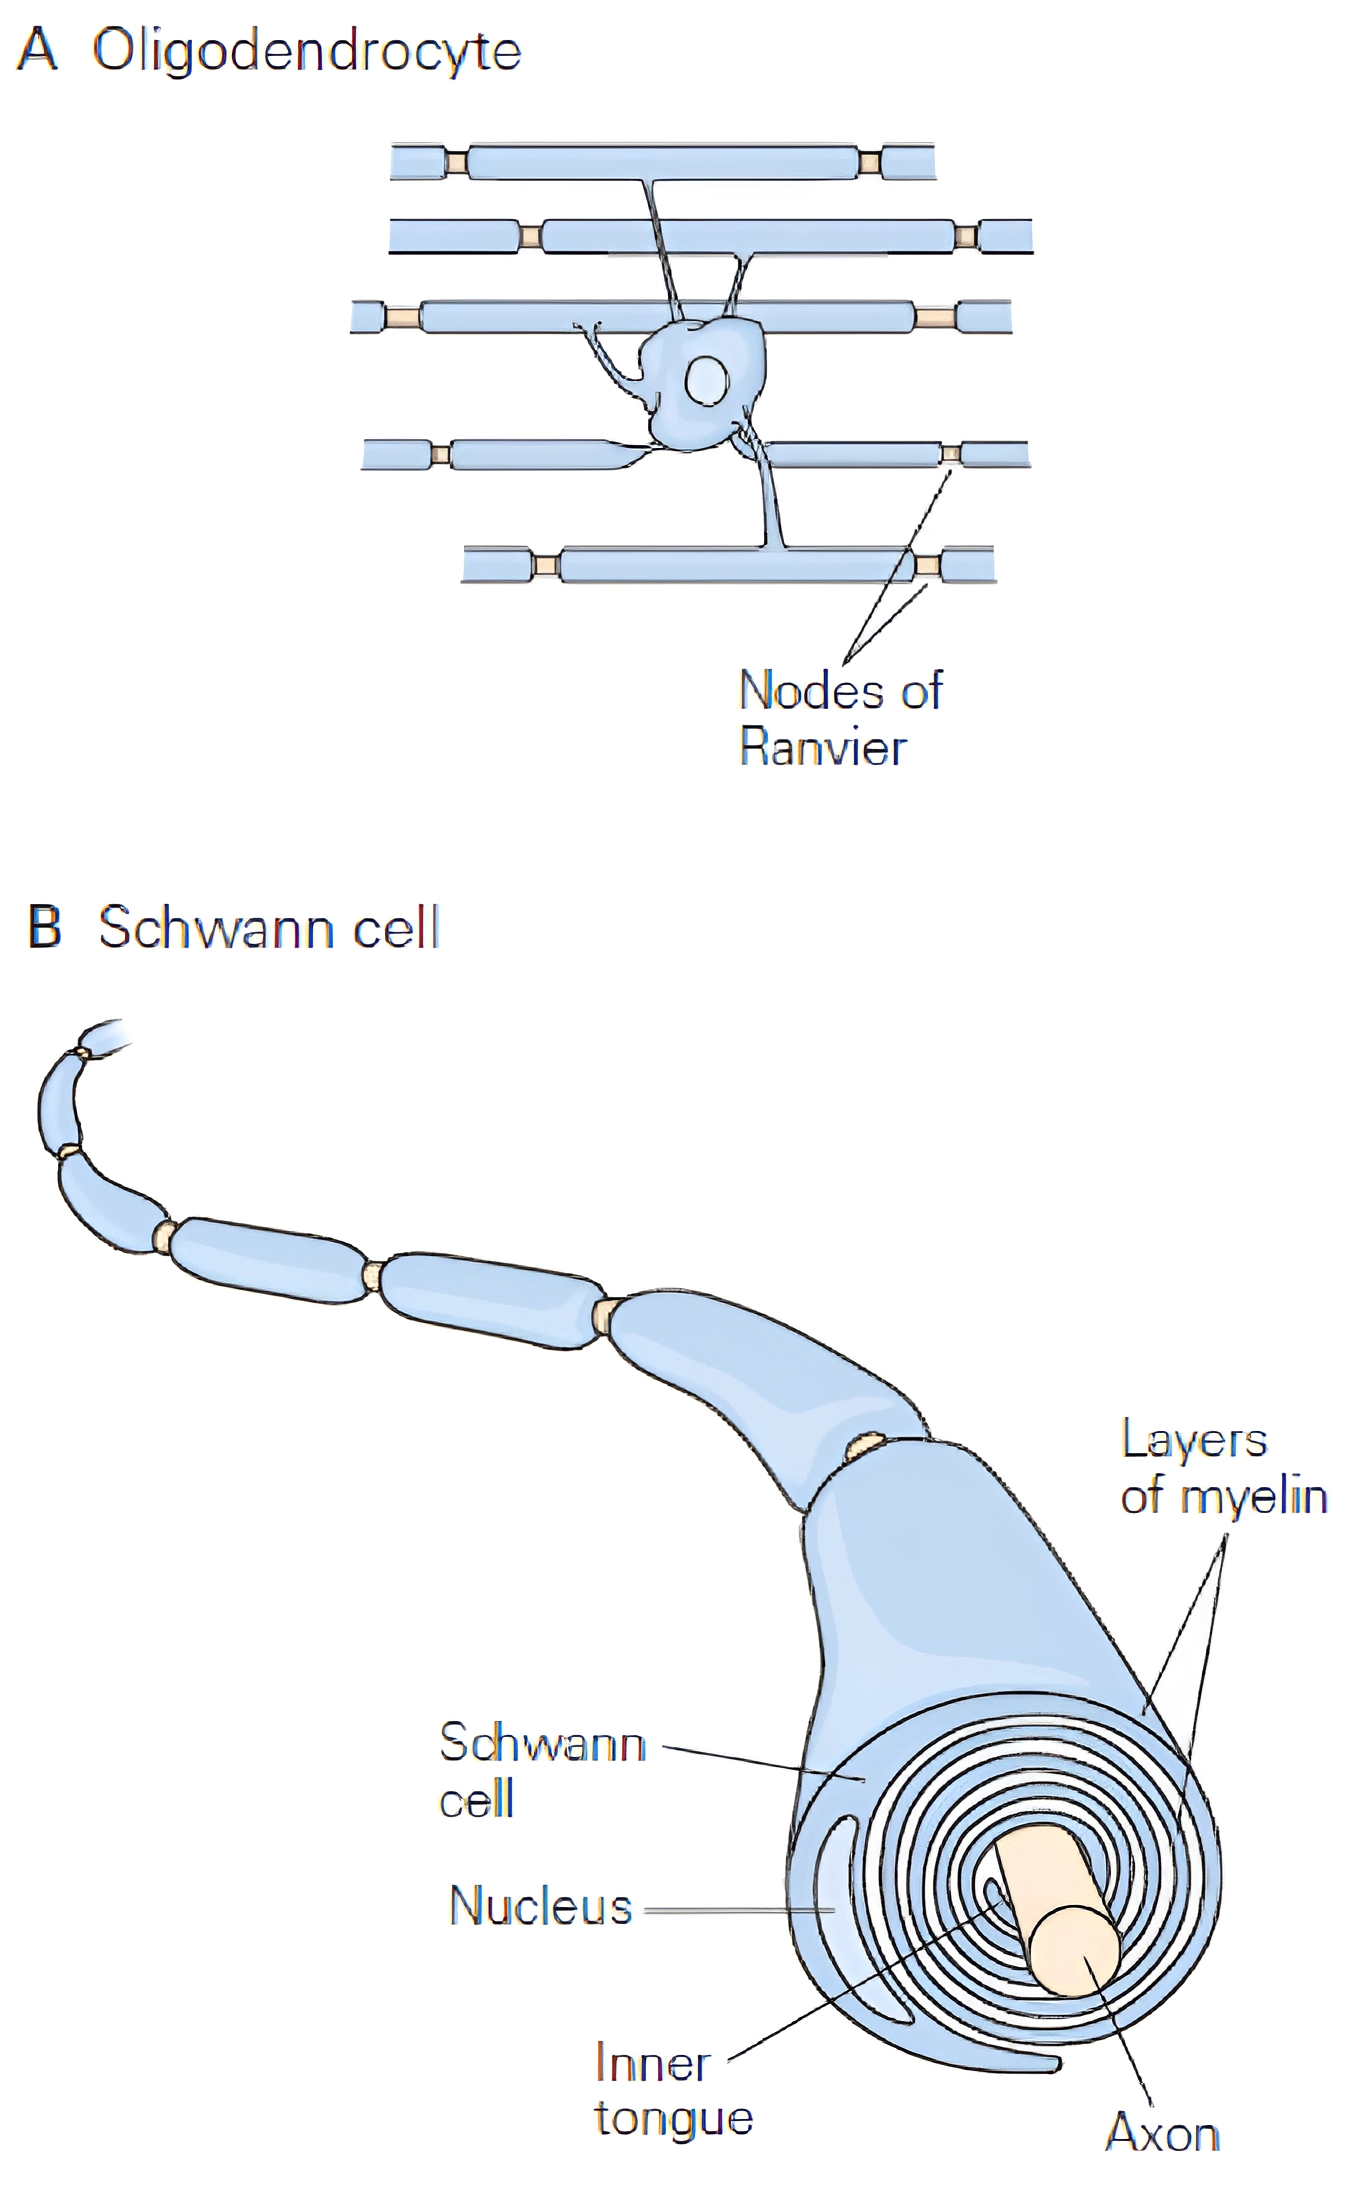
\includegraphics[width=\textwidth]{./img/insulation.png}
\end{minipage}



\subsection{Neurons / Nerve cells}
\marginnote{Neurons/Nerve cells}

A nervous system has around 100 billion neurons.
There are 100 distinct types of neurons varying in form, location, and interconnectivity.

Generally, a neuron does the following:
\begin{enumerate}
    \item Receives some information.
    \item Makes a decision.
    \item Passes it to other neurons.
\end{enumerate}

\begin{description}
    \item[Eukaryotic cell] \marginnote{Eukaryotic cell}
        A neuron is an eukaryotic cell. Therefore, it has:
        \begin{description}
            \item[Cell membrane] Membrane that separates the intracellular and extracellular space.
            \item[Cytoplasm] Intracellular fluid mainly made of proteins and ions of potassium, sodium, chloride, and calcium.
            \item[Extracellular fluid] Fluid in which the neuron sits. Similar composition of the cytoplasm.
            \item[Cell body/soma] Metabolic center of the cell.
        \end{description}

        \begin{figure}[h]
            \centering
            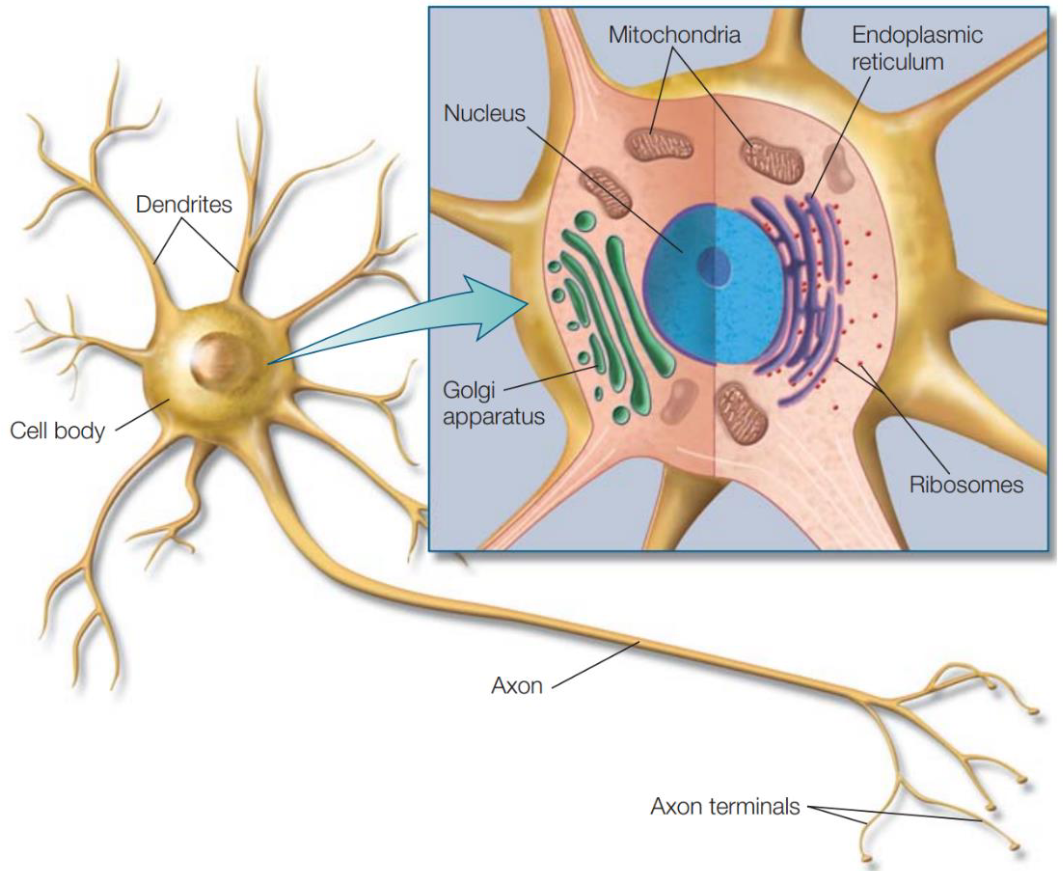
\includegraphics[width=0.5\textwidth]{img/neuron_eukaryotic.png}
            \caption{Neuron as an eukaryotic cell}
        \end{figure}
\end{description}

\begin{description}
    \item[Neuron-specific components] \phantom{}
        \begin{description}
            \item[Dendrites] \marginnote{Dendrites}
                Receives the outputs of other neurons.
                A neuron has multiple dendrites with different shapes depending on the type and location of the neuron.
            \item[Axon] \marginnote{Axon}
                Transmitting zone of the neuron that carries electrical signals from the dendrites to the synapses (from 0.1mm to 2m).
                A neuron has a single axon.
            \item[Synapses] \marginnote{Synapses}
                Represents the output zone of the neuron from where electrical or chemical signals can be transmitted to other cells.
                A neuron has multiple synapses.

                \begin{description}
                    \item[Presynaptic cell] Cell transmitting a signal.
                    \item[Postsynaptic cell] Cell receiving a signal.
                    \item[Synaptic cleft] Narrow space separating presynaptic and postsynaptic cells (i.e. the space separating two neurons).
                \end{description}
        \end{description}
\end{description}

\begin{figure}[H]
    \centering
    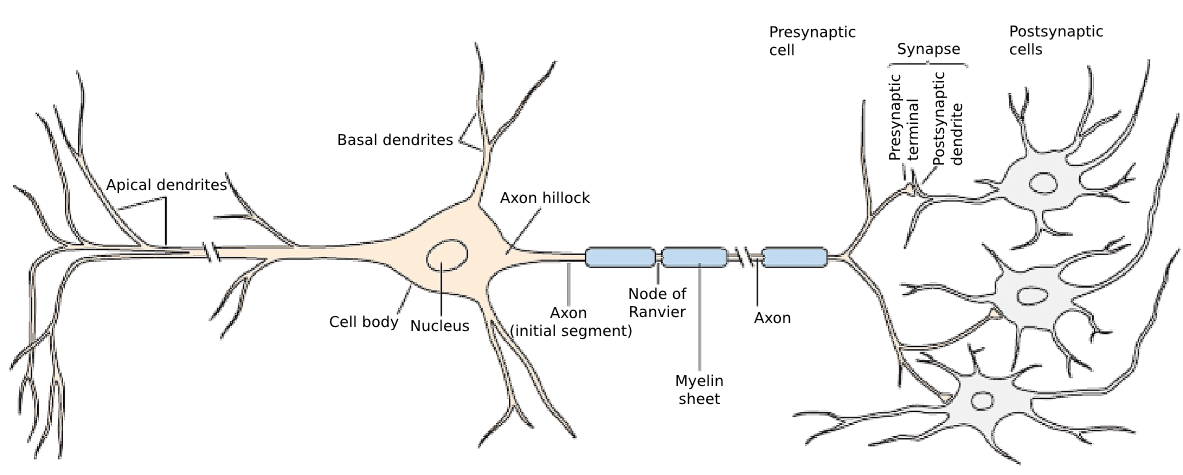
\includegraphics[width=0.9\textwidth]{img/neuron_specific.png}
    \caption{Neuron-specific components}
\end{figure}

There are three types of synapses:
\begin{descriptionlist}
    \item[Axosomatic] \marginnote{Axosomatic}
        Synapses that a neuron makes onto the cell body (soma) of another neuron.
    \item[Axodendritic] \marginnote{Axodendritic}
        Synapses that a neuron makes onto the dendrites of another neuron.
    \item[Axoaxonic] \marginnote{Axoaxonic}
        Synapses that a neuron makes onto the synapses of another neuron.
        In this case, the transmitting neuron can be seen as a signal modulator of the receiving neuron.
    \begin{figure}[h]
        \begin{subfigure}{.3\textwidth}
            \centering
            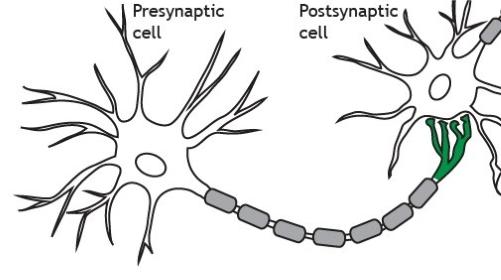
\includegraphics[width=\linewidth]{./img/axosomatic.png}
            \caption{Axosomatic}
        \end{subfigure}
        \begin{subfigure}{.3\textwidth}
            \centering
            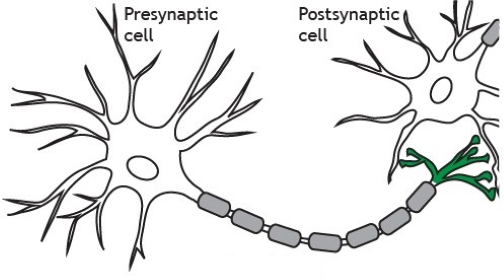
\includegraphics[width=\linewidth]{./img/axodendritic.png}
            \caption{Axodendritic}
        \end{subfigure}
        \begin{subfigure}{.3\textwidth}
            \centering
            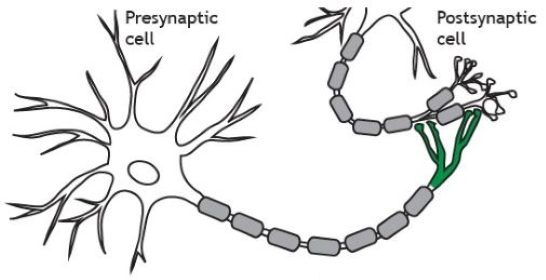
\includegraphics[width=\linewidth]{./img/axoaxonic.png}
            \caption{Axoaxonic}
        \end{subfigure}
    \end{figure}
\end{descriptionlist}

Neurons are divided into three functional categories:
\begin{descriptionlist}
    \item[Sensory neurons] \marginnote{Sensory neurons}
        Carry information from the body's peripheral sensors into the nervous system.
        Provides both perception and motor coordination.

    \item[Motor neurons] \marginnote{Motor neurons}
        Carry commands from the brain or the spinal cord to muscles and glands.

    \item[Interneurons] \marginnote{Interneurons}
        Intermediate neurons between sensory and motor neurons.
\end{descriptionlist}

\begin{description}
    \item[Principle of connectional specificity] \marginnote{Principle of connectional specificity}
        Neurons do not connect randomly but rather make specific connections at particular contact points.
\end{description}



\section{Information transfer within a neuron}


\subsection{Neuron functional regions}

In a neuron, there are four regions that handle signals:
\begin{descriptionlist}
    \item[Input zone] \marginnote{Input zone}
        Dendrites collect information from different sources
        in the form of \aclp{psp} (\acp{psp}).

    \item[Integration/trigger zone] \marginnote{Integration/trigger zone}
        \acp{psp} are summed at the axon hillock and an \ac{ap} is generated if a threshold (-55mV) has been exceeded.

    \item[Conductive zone] \marginnote{Conductive zone}
        The \ac{ap} is propagated through the axon.

    \item[Output zone] \marginnote{Output zone}
        Synapses transfer information to other cells.

        \begin{description}
            \item[Chemical synapses] The frequency of \acp{ap} determines the amount of neurotransmitters released.
            \item[Electrical synapses] The \ac{ap} is directly transmitted to the next neurons.
        \end{description}

    \begin{figure}[h]
        \centering
        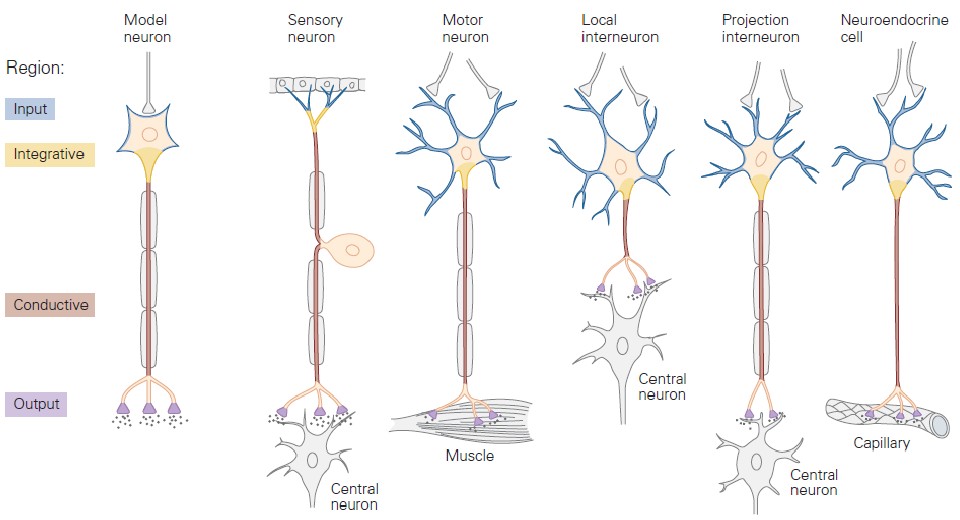
\includegraphics[width=0.8\textwidth]{./img/neuron_transmission.png}
        \caption{Transmitting regions of different types of neurons}
    \end{figure}

    \begin{figure}[h]
        \centering
        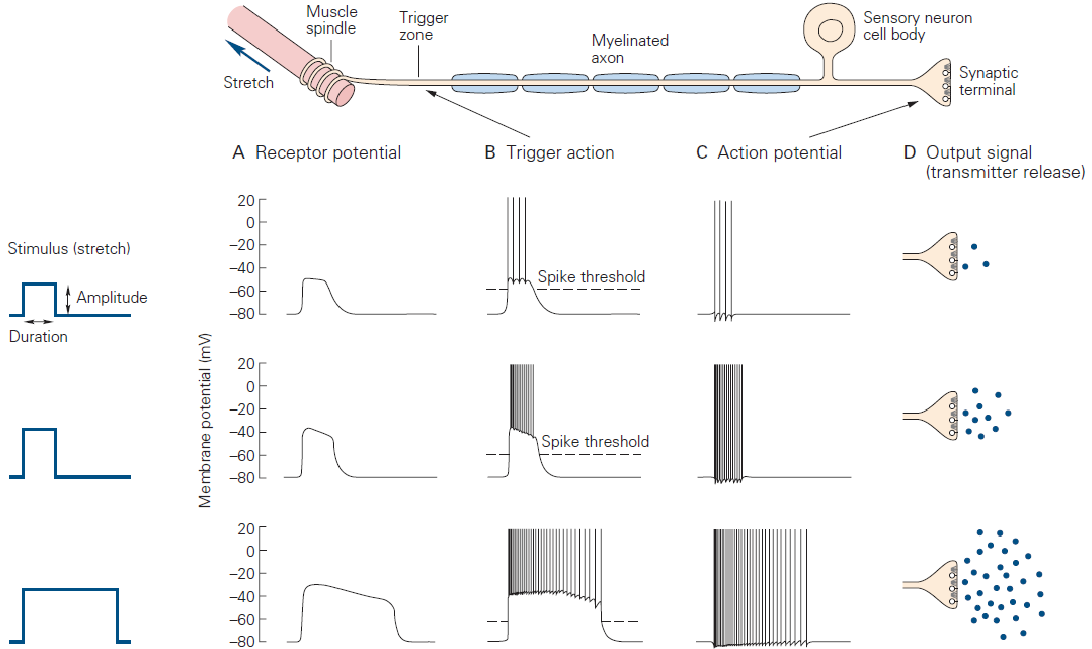
\includegraphics[width=0.8\textwidth]{./img/neuron_transmission2.png}
        \caption{Signal from the input to the output zones}
    \end{figure}
\end{descriptionlist}


\subsection{Neuron transmission signals}

\begin{description}
    \item[Resting membrane potential] \marginnote{Resting membrane potential}
        In a resting neuron, the voltage inside the cell is more negative ($-70$mV) than the outside.
        This allows the creation of an electrical signal when needed.

    \item[\Acl{psp} (\ac{psp})] \marginnote{\Acl{psp} (\ac{psp})}
        Small change in the membrane potential that alters the resting voltage of the cell.
        
        A \ac{psp} can be:
        \begin{descriptionlist}
            \item[Excitatory \ac{psp} (\acs{epsp})] \marginnote{Excitatory \ac{psp}}
                Has a depolarizing role: produces a decrease in the membrane potential (i.e. increases voltage inside the cell), 
                therefore enhancing the ability to generate an \ac{ap}.

            \item[Inhibitory \ac{psp} (\acs{ipsp})] \marginnote{Inhibitory \ac{psp}}
                Has a hyperpolarizing role: produces an increase in the membrane potential (i.e. reduces voltage inside the cell), 
                therefore reducing the ability to generate an \ac{ap}.
        \end{descriptionlist}

        A \ac{psp} has the following properties:
        \begin{itemize}
            \item The amplitude and duration of the signal are determined by the size of the stimulus that caused it.
                Overall, the amplitude is small.
            \item The signal is passively conducted through the cytoplasm, therefore it decays with distance and is able to travel 1mm at most.
            \item A single \acs{epsp} is not enough to fire a neuron. Multiple \acp{psp} are summed at the axon hillock.
                There are two types of summation:
                \begin{descriptionlist}
                    \item[Spatial summation] Sum of the \acp{psp} received at the same time.
                    \item[Temporal summation] Sum of the \acp{psp} received at different time points.
                \end{descriptionlist}

                \begin{remark}
                    The fact that a single \ac{epsp} is not enough to fire a neuron prevents a response to every single stimulus.
                \end{remark}
        \end{itemize}

    \item[\Acl{ap} (\ac{ap})] \marginnote{\Acl{ap} (\ac{ap})}
        Signal generated when the sum of \acp{epsp} exceeds a fixed threshold of $-55$mV (all-or-none).

        \begin{description}
            \item[Saltatory conduction] \marginnote{Saltatory conduction}
                Mechanism that allows a fast propagation on long distances of \acp{ap}.
                \begin{enumerate}
                    \item Depolarization causes the sodium ion (Na+) channels located in the nodes of Ranvier of the axon to gradually open.
                    \item Na+ flows into the neuron and further depolarizes it until the Na+ equilibrium potential is reached.
                    \item With Na+ equilibrium, Na+ channels close and potassium ion (K+) channels open.
                    \item K+ flows into the neuron and restores the membrane potential until the K+ equilibrium potential is reached.
                    \item With K+ equilibrium, K+ channels close and 
                        the membrane potential of the neuron is more negative than the resting potential (hyperpolarization).
                        It will gradually return to its resting potential.
                        \begin{remark}
                            During hyperpolarization, Na+ channels cannot open (refractory period).
                            This has two implications:
                            \begin{itemize}
                                \item It limits the number of times a neuron can fire in a given time.
                                \item Guarantees a unidirectional electrical current flow 
                                    (\textbf{Principle of dynamic polarization}).\marginnote{Principle of dynamic polarization} 
                            \end{itemize}
                        \end{remark}
                \end{enumerate}

                \begin{figure}[H]
                    \begin{subfigure}{.45\textwidth}
                        \centering
                        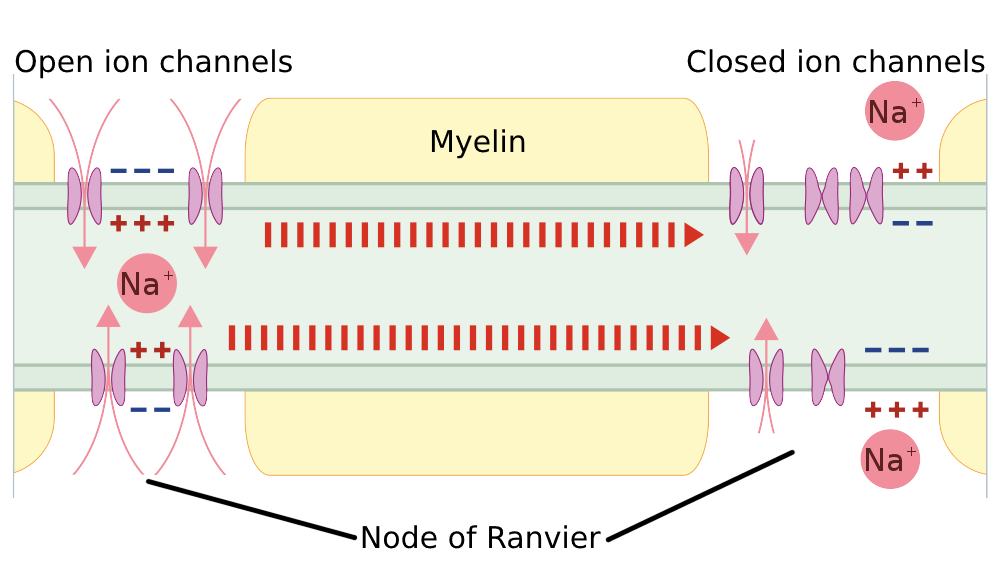
\includegraphics[width=0.85\textwidth]{./img/saltatory_conduction.png}
                        \caption{Ion channels along the axon}
                    \end{subfigure}
                    \begin{subfigure}{.45\textwidth}
                        \centering
                        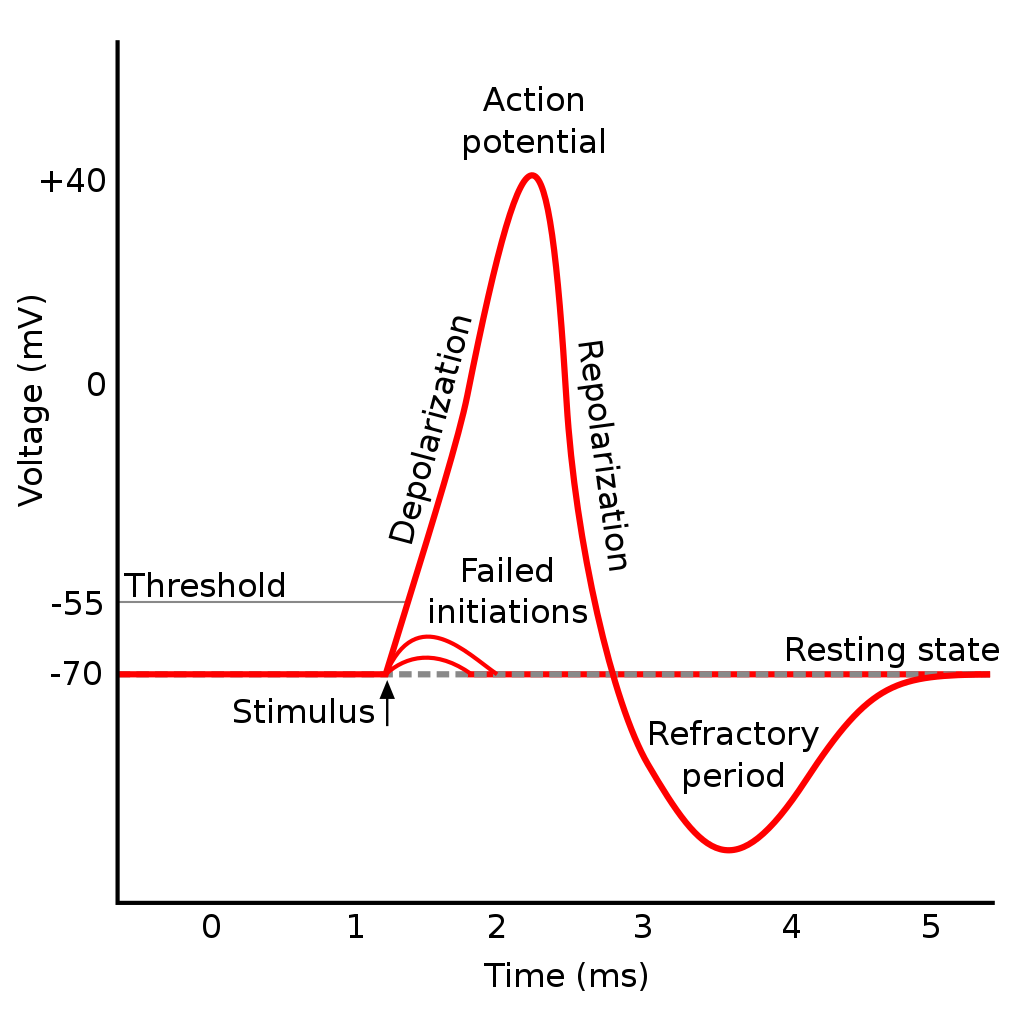
\includegraphics[width=0.8\textwidth]{./img/action_potential.png}
                        \caption{Triggering of an action potential}
                    \end{subfigure}
                \end{figure}
        \end{description}


        \begin{remark}
            As the signal is constantly regenerated, 
            \Acp{ap} have similar amplitude and duration in all neurons, regardless of the characteristics of the input \acp{psp}.
            Therefore, the only way an \ac{ap} has to carry information is by varying frequency and firing duration, making it a binary signal.
        \end{remark}
\end{description}

\begin{example}
    Seizures are caused by misfiring neurons.
\end{example}



\section{Information transfer between two neurons}


\subsection{Electrical synapse}

\begin{minipage}{0.55\textwidth}
    \begin{description}
        \item[Structure] \marginnote{Electrical synapse}
            The neuronal membranes of the presynaptic and postsynaptic neurons are in contact at \textbf{gap junctions} and
            the cytoplasm of the two neurons is virtually continuous through connecting \textbf{pores}.
    \end{description}
\end{minipage}
\begin{minipage}{0.35\textwidth}
    \centering
    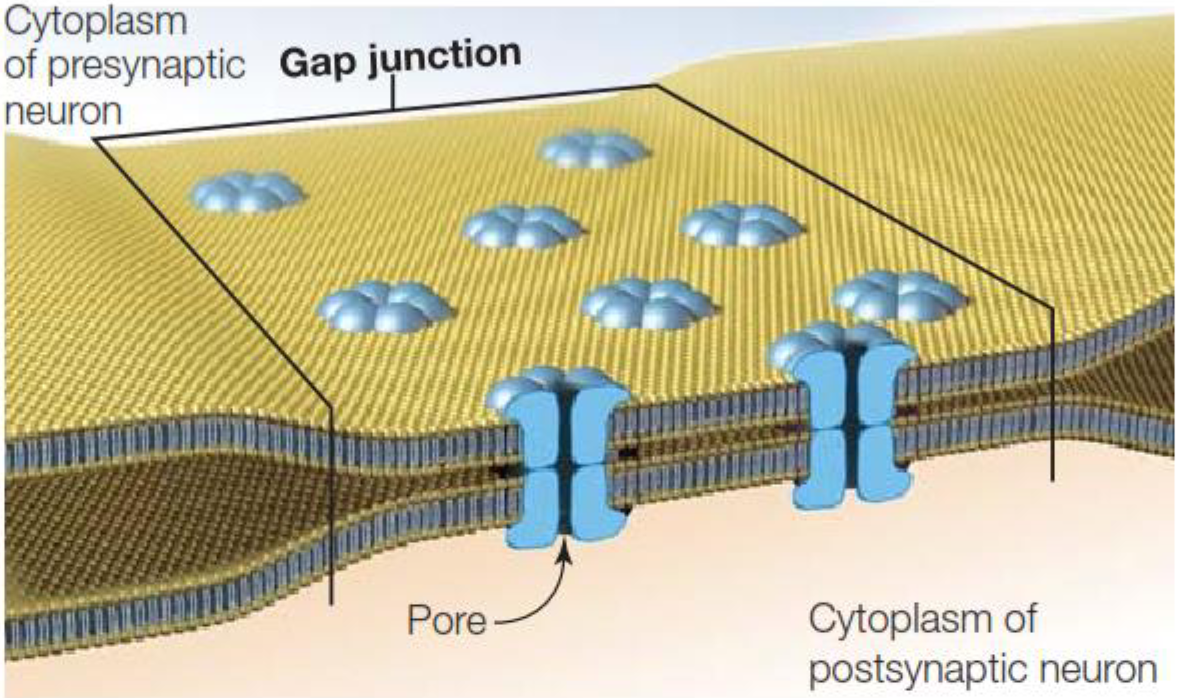
\includegraphics[width=\linewidth]{./img/electric_synapse.png}
\end{minipage}

\begin{description}
    \item[Functioning]
        The two neurons are \textbf{isopotential} (i.e. they have the same membrane potential) and 
        the ions of the presynaptic neurons are instantaneously transmitted to the postsynaptic neuron.

    \item[Properties] \phantom{}
        \begin{itemize}
            \item Fast transmission.
            \item Allows for synchronous operations involving groups of neurons.
            \item The strength of the signal cannot be modulated.
        \end{itemize}
\end{description}


\subsection{Chemical synapse}

\begin{description}
    \item[Structure] \marginnote{Chemical synapse}
        The synaptic cleft separates the presynaptic and postsynaptic neurons.
        \begin{description}
            \item[Neurotransmitter] 
                Chemical substance received by the receptors of the postsynaptic neuron.

                The effect of a neurotransmitter is decided by the receiving receptor and not by the cell transmitting it.

            \item[Presynaptic terminals] 
                Swellings at the end of the axon that contain synaptic vesicles.

            \item[Synaptic vesicles] 
                Vesicles containing neurotransmitter molecules.
        \end{description}

    \item[Functioning] 
        The release of neurotransmitter molecules is based on the following steps:
        \begin{enumerate}
            \item An action potential arriving at the terminal of a presynaptic axon causes the calcium ion (Ca$^{2+}$) voltage-gates to open.
            \item Ca$^{2+}$ flow into the cell and 
                cause the synaptic vesicles to bind to the cell membrane to release neurotransmitters into the synaptic cleft.
            \item Neurotransmitters cross the synaptic cleft and bind to the receptors of the postsynaptic neuron.
                Depending on the neurotransmitter and the receiving receptor, there might be a generation of \ac{epsp} or \ac{ipsp}.
        \end{enumerate}

        \begin{center}
            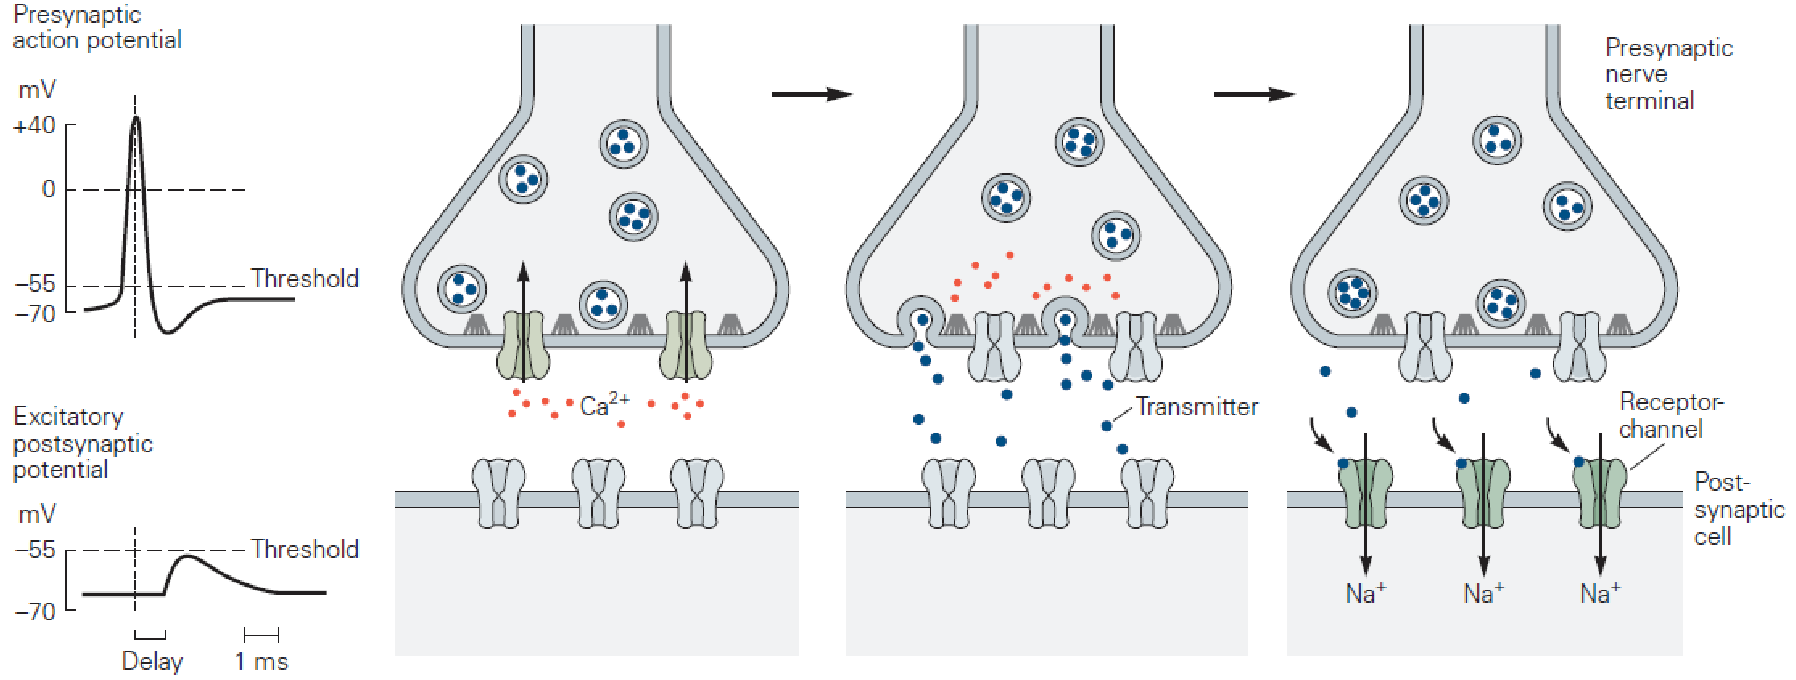
\includegraphics[width=0.9\linewidth]{./img/chemical_synapse.png}
        \end{center}

        When a receptor recognizes the neurotransmitter, it is released back into the synaptic cleft.
        To avoid a constant stimulation of the receptors, neurotransmitters are inactivated:
        \begin{itemize}
            \item The synaptic terminal can reuptake neurotransmitters through transporter proteins.
            \item Neurotransmitters might degenerate or be broken down by special enzymes.
            \item Neurotransmitters can be released far away from the site of the receptors.
        \end{itemize}

    \item[Properties] \phantom{}
        \begin{itemize}
            \item Slow transmission.
            \item The signal can be modulated.
            \item Has specific effects depending on the neurotransmitter and the receptors.
        \end{itemize}
\end{description}



\section{Neural circuit}

\begin{description}
    \item[Neural circuit] \marginnote{Neural circuit}
        Group of interconnected neurons that process a specific kind of information.

        \begin{remark}
            The behavioral function of each neuron is determined by its connections.
        \end{remark}

    \item[Types of neurons] \phantom{}
        \begin{description}
            \item[Sensory neuron] \marginnote{Sensory neuron}
                Carry information from the peripheral sensors to the nervous system for both perception and motor coordination.
        
            \item[Motor neuron] \marginnote{Motor neuron}
                Carry information from the nervous system to muscles and glands.
            
            \item[Interneuron] \marginnote{Interneuron}
                Intermediate neurons between sensory and motor neurons.
        \end{description}
\end{description}

\begin{remark}
    In vertebrates, a stimulus causes multiple neural pathways to simultaneously encode different information.
    This allows for parallel processing to increase both the speed and reliability of the information transfer.
\end{remark}

\begin{description}
    \item[Neural pathways types] \phantom{}
        \begin{description}
            \item[Divergent pathway] \marginnote{Divergent pathway}
                One neuron activates many target cells.
                Typically happens at the input stages of the nervous system
                to ensure that a single neuron has a wide and diverse influence.

            \item[Convergent pathway] \marginnote{Convergent pathway}
                Many neurons activate a single target cell.
                Typically happens at the output stages of the nervous system 
                to ensure that a motor neuron is activated only when a sufficient number of neurons are firing.
        \end{description}

    \item[Neuron firing types] \phantom{}
        \begin{description}
            \item[Excitatory neuron] \marginnote{Excitatory neuron}
                Neurons that produce signals that increase the probability of firing of the postsynaptic neurons.
                
            \item[Inhibitory neuron] \marginnote{Inhibitory neuron}
                Neurons that produce signals that decrease the probability of firing of the postsynaptic neurons.
                
                \begin{description}
                    \item[Feed-forward inhibition] 
                        Excitatory neurons connected to inhibitory interneurons to block other downstream neurons.
                        Allows to enhance the active pathway and to block other antagonist actions.
                        \begin{figure}[H]
                            \centering
                            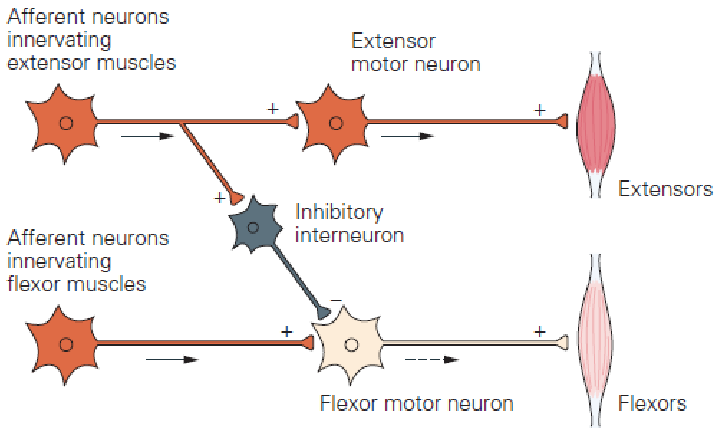
\includegraphics[width=0.4\textwidth]{./img/feedforward_inhibition.png}
                            \caption{Example of feed-forward inhibition}
                        \end{figure}

                    \item[Feed-back inhibition] 
                        Excitatory neurons connected to inhibitory interneurons that return to the same neurons to inhibit them.
                        Prevents the overload of neurons or muscles.
                        \begin{figure}[H]
                            \centering
                            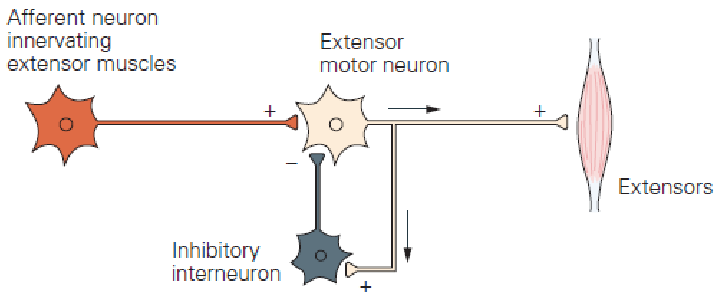
\includegraphics[width=0.4\textwidth]{./img/feedback_inhibition.png}
                            \caption{Example of feed-back inhibition}
                        \end{figure}
                \end{description}
        \end{description}
\end{description}



\begin{casestudy}[Knee-jerk reflex]
    By tapping the patellar tendon (below the kneecap), the following happens:
    \begin{enumerate}
        \item The sensory information is conveyed from the muscle to the spinal cord (central nervous system).
        \item The nervous system issues motor commands to the muscles which results in the knee jerk.
        \item Inhibitory commands are issued to stop antagonist muscles.
    \end{enumerate}

    \begin{center}
        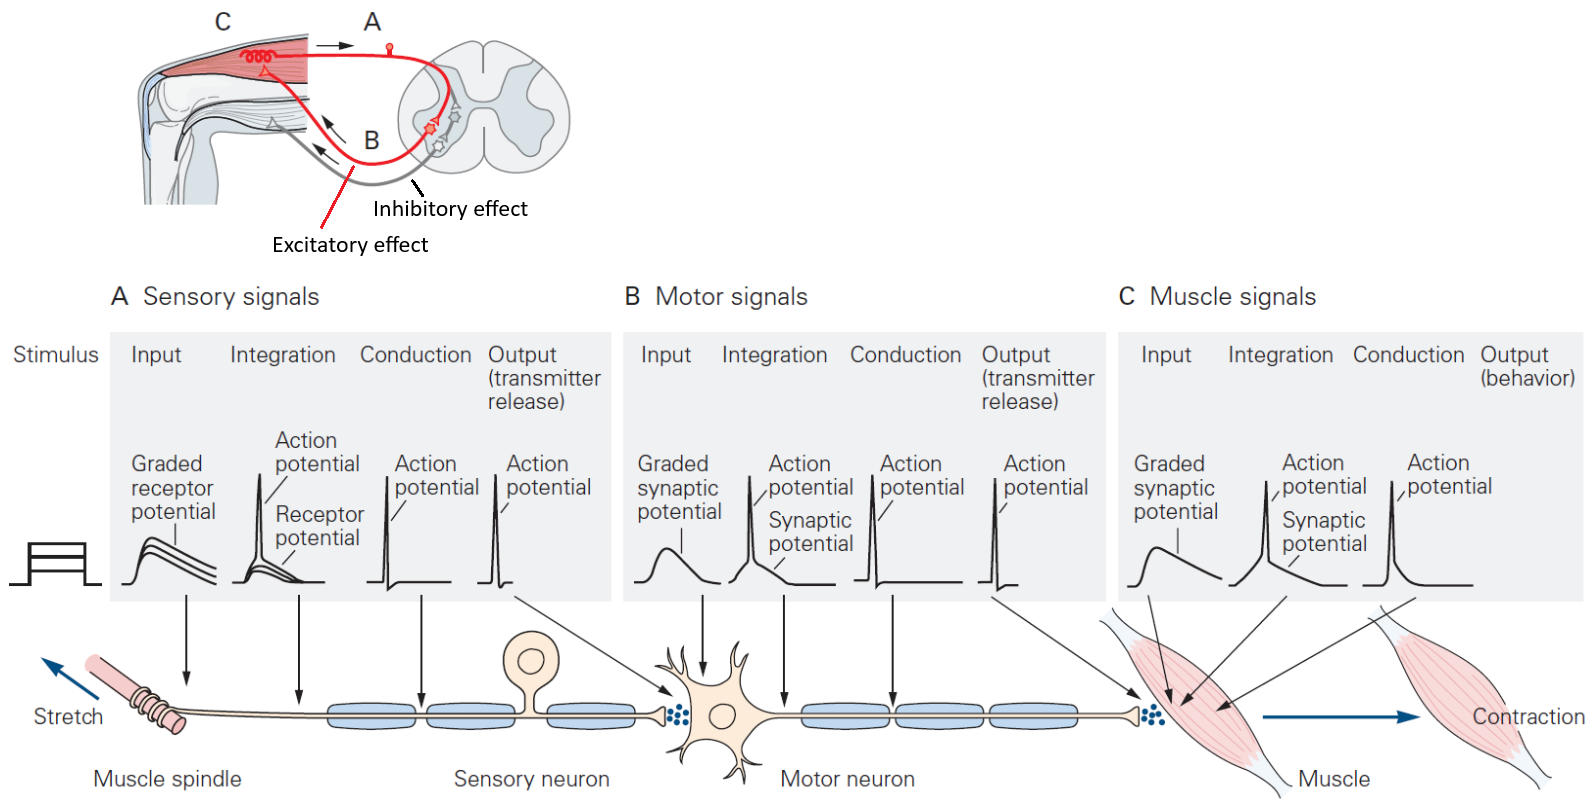
\includegraphics[width=0.8\textwidth]{./img/knee_jerk.png}
    \end{center}
\end{casestudy}


\section{Neural system}

\begin{figure}[H]
    \centering
    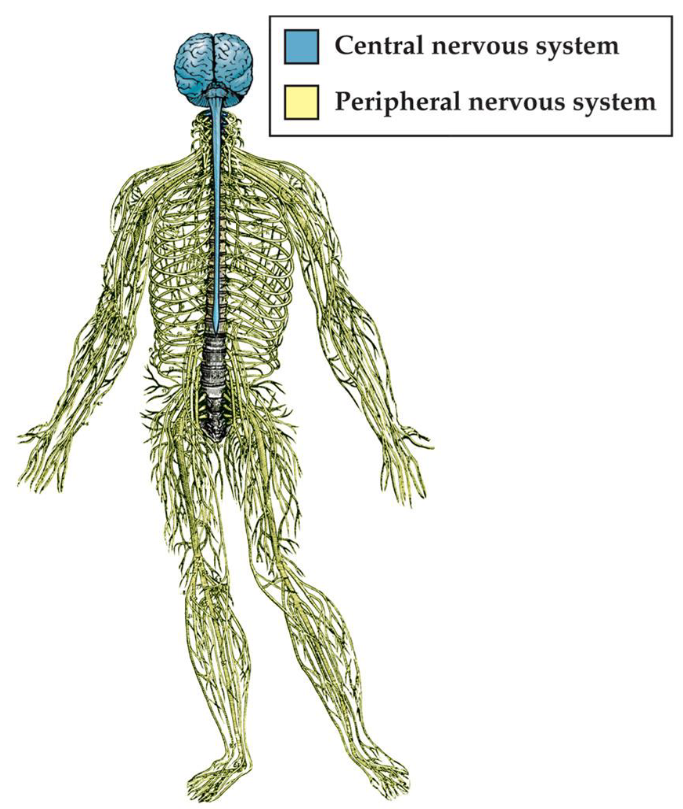
\includegraphics[width=0.3\textwidth]{./img/neural_system.png}
    \caption{Composition of the nervous system}
\end{figure}


\subsection{\Acl{pns} (\acs{pns})}

The \acl{pns} is composed of:
\begin{descriptionlist}
    \item[Nerves] \marginnote{Nerves}
        Groups of axons and glia.

    \item[Ganglia] \marginnote{Ganglia}
        Groups of neuron bodies outside the \acl{cns}
\end{descriptionlist}

The \ac{pns} has the following functions:
\begin{itemize}
    \item Delivers sensory information to the \acl{cns}.
    \item Carries commands from the \acl{cns} to the muscles.
    \item Supplies the \acl{cns} with information regarding both the external and internal environment.
\end{itemize}

The \ac{pns} has the following divisions:
\begin{descriptionlist}
    \item[Somatic nervous system] \marginnote{Somatic nervous system} \phantom{}
        \begin{itemize}
            \item Sensory neurons that receive information from the skin, muscles, and joints.
            \item Converts perceived spatial and physical information into electrical signals for the \acl{cns} to process.
            \item Controls the voluntary muscles.
        \end{itemize}

    \item[Autonomic nervous system] \marginnote{Autonomic nervous system} \phantom{}
        \begin{itemize}
            \item Controls internal organs (viscera), the vascular system, and involuntary muscles and glands.
            \item Divided into three systems:
                \begin{descriptionlist}
                    \item[Sympathetic system] \marginnote{Sympathetic system}
                        Operates antagonistically against the parasympathetic system.
                        Handles the body's response to stress (using norepinephrine).

                        Physically, the sympathetic system originates from the spinal cord. 
                        Its ganglia are closer to the spinal cord,
                        therefore the axons from the \acl{cns} to the ganglia are shorter than the axons from the ganglia to the organs.

                        \begin{example}
                            Stimulates adrenal glands to prepare the body for action (fight or flight),
                            increases heart rate,
                            diverts the blood from the digestive tract to the somatic musculature, \dots
                        \end{example}

                    \item[Parasympathetic system] \marginnote{Parasympathetic system}
                        Operates antagonistically against the sympathetic system.
                        Acts to preserve the body's resources and restore homeostasis (using acetylcholine).

                        Physically, the parasympathetic system originates from the base of the brain and from the sacral spinal cord.
                        Its ganglia are outside the spinal cord, sometimes inside the affected organs,
                        therefore the axons from the \acl{cns} to the ganglia are longer than the axons from the ganglia to the organs.

                        \begin{example}
                            Slows heart rate, stimulates digestion, \dots
                        \end{example}

                    \item[Enteric system] \marginnote{Enteric system}
                        Controls the involuntary muscles of the gut.
                \end{descriptionlist}
        \end{itemize}
\end{descriptionlist}



\subsection{\Acl{cns} (\acs{cns})}

\begin{description}
    \item[Meninges] \marginnote{Meninges}
        Three layers of membrane protecting the brain and the spinal cord.
        \begin{descriptionlist}
            \item[Dura mater] The outermost and thickest layer.
            \item[Arachnoid mater] The middle layer.
            \item[Pia mater] The innermost and most delicate layer. It adheres to the brain's surface.
        \end{descriptionlist}

    \item[Cerebrospinal fluid] \marginnote{Cerebrospinal fluid}
        Fluid that allows the brain to float and prevents it from simply sitting on the skull surface.
        It also reduces the shock to the brain and the spinal cord in case of rapid accelerations/decelerations.

        The fluid is located in:
        \begin{itemize}
            \item The space between the arachnoid mater and the pia mater.
            \item The brain ventricles.
            \item Cisterns and sulcis.
            \item The central canal of the spinal cord.
        \end{itemize}

    \item[Blood-brain barrier] \marginnote{Blood-brain barrier}
        Barrier between the brain's capillaries and the brain's tissue.
        It protects against pathogens and toxins.

        \begin{remark}
            The effectiveness of the barrier also prevents drugs to treat mental and neurological disorders from passing through.
        \end{remark}

    \item[Spinal cord] \marginnote{Spinal cord}
        Acts as a relay for the information coming in and out of the brain.
        It is enclosed in the vertebral column.
\end{description}

\begin{remark}
    Most pathways in the \ac{cns} are bilaterally symmetrical: 
    the sensory and motor activities of one side of the body are handled by the cerebral hemisphere on the opposite side.
\end{remark}

\begin{description}
    \item[Brain] \marginnote{Brain}
    
    \begin{minipage}{0.6\textwidth}
        \begin{description}
            \item[Brain stem] \marginnote{Brain stem}
                Regulates basic life functions such as blood pressure, respiration, and sleep/wakefulness.
                It is divided into three sections:
                \begin{itemize}
                    \item Medulla.
                    \item Pons.
                    \item Midbrain.
                \end{itemize}
        \end{description}
    \end{minipage}
    \begin{minipage}{0.35\textwidth}
        \centering
        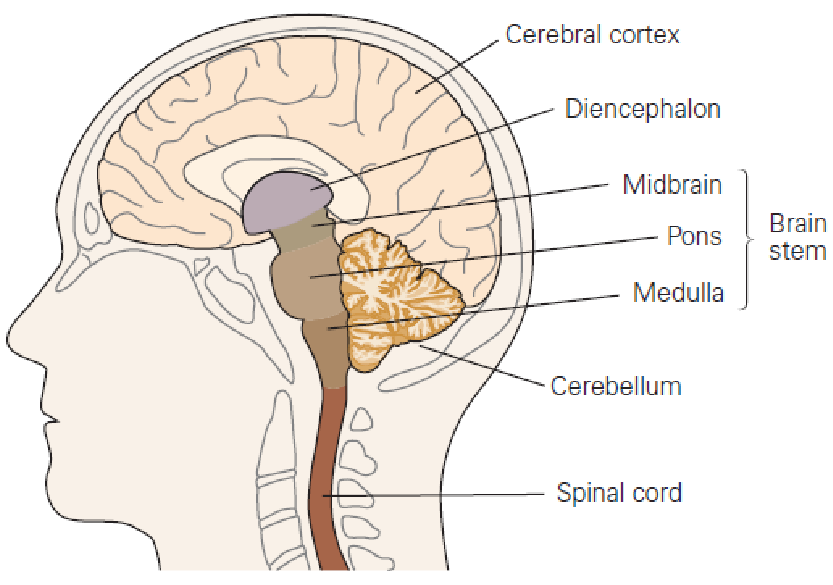
\includegraphics[width=\linewidth]{./img/brain_sections.png}
    \end{minipage}

    \begin{description}
        \item[Cerebellum] \marginnote{Cerebellum}
            Contains lots of neurons and is responsible for:
            \begin{itemize}
                \item Maintaining posture.
                \item Coordinating head, eye, and arm movement.
                \item Regulating motor control (i.e. adjustments to the movement).
                \item Learning motor skills.
            \end{itemize}

        \item[Diencephalon] \marginnote{Diencephalon} 
            \phantom{}\\
            \begin{minipage}{0.6\linewidth}
                \begin{description}
                    \item[Thalamus] \marginnote{Thalamus}
                        Sorts incoming sensory information (except the sense of smell) of the \acl{pns} and 
                        sends them to the sensory regions of the cerebral hemispheres.
                    \item[Hypothalamus] \marginnote{Hypothalamus}
                        Regulates the autonomic nervous system and homeostasis through the pituitary gland (which releases hormones).
                        Handles the motivation system of the brain by favoring behaviors the organism finds rewarding.
                \end{description}
            \end{minipage}
            \begin{minipage}{0.35\linewidth}
                \centering
                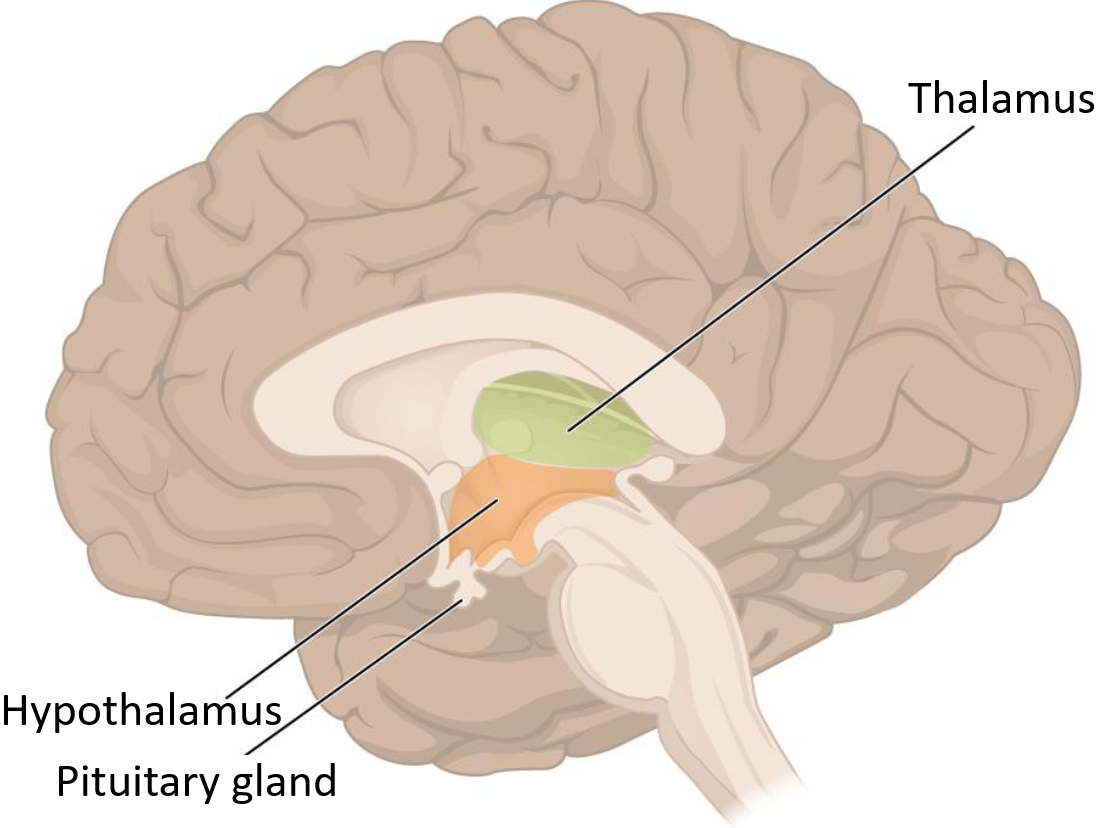
\includegraphics[width=\linewidth]{./img/diencephalon.png}
            \end{minipage}

        \item[Telencephalon/Cerebral hemispheres] \marginnote{Telencephalon/Cerebral hemispheres}
            Consists of:
            \begin{description}
                \item[Cerebral cortex] 
                    Made of gray matter (body of neurons).

                \item[White matter] 
                    (axons and glial cells).

                \item[Basal ganglia] \marginnote{Basal ganglia}
                    Receive inputs from sensory and motor areas and 
                    mostly send them through the thalamus to the frontal lobe.

                    They have a crucial role in motor control and reinforcement learning.
                    This happens through two pathways:
                    \begin{descriptionlist}
                        \item[Direct pathway] When active, it causes the disinhibition of the thalamus and has the consequence of initializing movement.
                        \item[Indirect pathway] When active, it causes the inhibition of the thalamus and consequently inhibits movement.
                    \end{descriptionlist}
                    To activate the direct pathway and inhibit the indirect pathway, the substantia nigra pars compacta (SNc) releases the neurotransmitter dopamine.

                    \begin{example}[Parkinson's disease]
                        In patients affected by Parkinson's disease, the dopamine-related neurons in the SNc are lost causing
                        an overactivation of the indirect pathway that inhibits movement.
                    \end{example}

                \item[Amygdala] \marginnote{Amygdala}
                    Responsible for recognizing a stimulus and reacting to it.
                    Involved in attention, perception, value representation, decision-making, learning, memory, \dots

                \item[Hippocampus] \marginnote{Hippocampus}
                    Responsible for long-term memory and spatial memory.
            \end{description}

        \item[Cerebral cortex] \marginnote{Cerebral cortex}
            Surface of the brain which covers around 2.2m$^2$ to 2.4m$^2$.
            To cover more surface, the cortex has infoldings (sulci and gyri) which also allow to connect neurons with shorter axons.

            There are two symmetrical hemispheres connected through the corpus callosum and four different lobes.

            \begin{figure}[H]
                \centering
                \begin{subfigure}{0.25\linewidth}
                    \centering
                    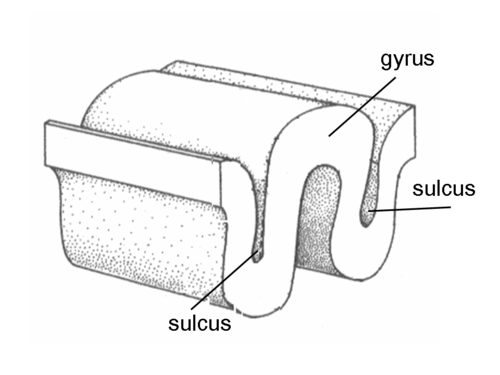
\includegraphics[width=\linewidth]{./img/brain_surface.png}
                    \caption{Visualization of sulci and gyri}
                \end{subfigure}
                \begin{subfigure}{0.35\linewidth}
                    \centering
                    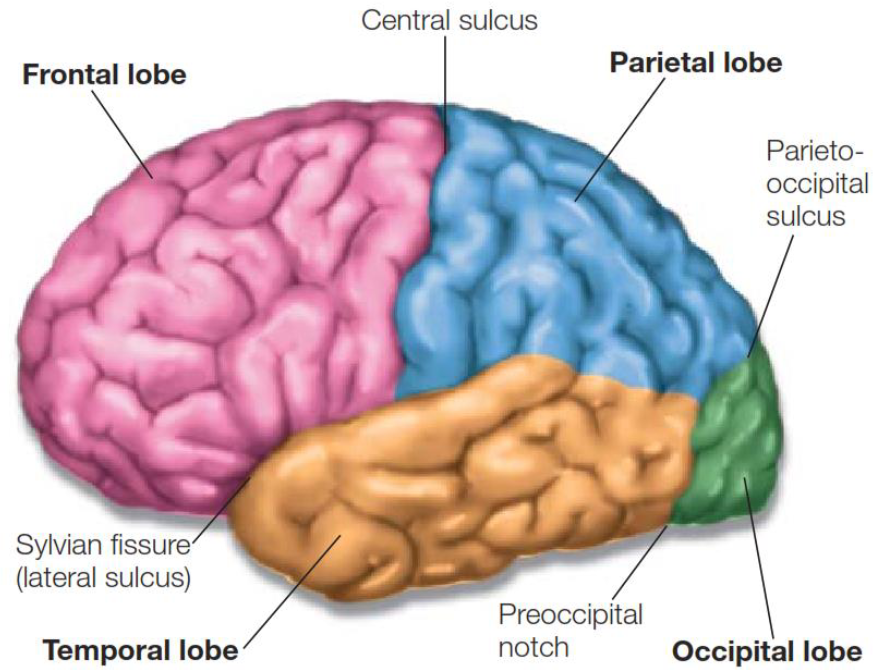
\includegraphics[width=\linewidth]{./img/brain_lobes.png}
                    \caption{Lobes of the brain}
                \end{subfigure}
            \end{figure}

            \begin{description}
                \item[Frontal lobe] \marginnote{Frontal lobe}
                    \phantom{}
                    \begin{description}
                        \item[Motor cortex] \phantom{}
                            \begin{itemize}
                                \item Planning and execution of movement.
                                \item Contains neurons that directly activate somatic movement neurons in the spinal cord.
                            \end{itemize}

                        \item[Prefrontal cortex] \phantom{}
                            \begin{itemize}
                                \item Long-term planning.
                                \item Decision making.
                                \item Motivation and value.
                            \end{itemize}
                    \end{description}
                

                \item[Parietal lobe] \marginnote{Parietal lobe}
                    Receives and integrates information from the outside world, the body, and memory.

                    \begin{description}
                        \item[Somatosensory cortex]
                            Receives information regarding touch, pain, temperature, and limb position.
                    \end{description}

                    \begin{remark}
                        Neurons responsible for a specific part of the body are clustered together.
                    \end{remark}


                \item[Occipital lobe] \marginnote{Occipital lobe}
                    \begin{description}
                        \item[Visual cortex] 
                            Responsible for vision. 
                            Encodes features like luminance, spatial frequency, orientation, motion, \dots
                    \end{description}

                    \begin{remark}
                        Neurons responsible for processing a specific feature are clustered together.
                    \end{remark}


                \item[Temporal lobe] \marginnote{Temporal lobe}
                    \begin{description}
                        \item[Auditory cortex]
                            Responsible for processing sound.
                    \end{description}

                    \begin{remark}
                        Neurons responsible for processing a specific sound frequency are clustered together.
                    \end{remark}

                \item[Association cortex] \marginnote{Association cortex}
                    Portion of the cortex that has neither sensory nor motor responsibility.
                    Receives and integrates inputs from many cortical areas.

                    \begin{description}
                        \item[Multisensory neuron]
                            Cell activated by multiple sensory modalities.
                    \end{description}
            \end{description}
    \end{description}
\end{description}
    \chapter{Reinforcement learning}


\section{Definitions}

\Acl{rl} (\acs{rl}) methods aim to maximize future reward by mapping the possible states of an environment into actions.

\begin{description}
    \item[Optimal decision making] \marginnote{Optimal decision making}
        Aims to maximize rewards and minimize punishments.

        \begin{remark}
            This is a difficult task as the outcome might be delayed or depend on a series of actions.
            
            \begin{descriptionlist}
                \item[Credit assignment problem]
                    Determine how the various factors involved in making a decision contributed to the success or failure of it.
            \end{descriptionlist}
        \end{remark}
\end{description}

\begin{remark}
    Multiple competing sub-systems contribute to learning and controlling behavior in animals.

    \begin{example}[Freud's theory of the mind structure]
        The mind is composed of three structures:
        \begin{descriptionlist}
            \item[Ego]
                Mainly works at the conscious level.
                Rational part of the mind that mediates id impulses and superego inhibitions.

            \item[Superego] 
                Mainly works at the preconscious level.
                Includes one's ideals and morals. Strives for perfection.

            \item[Id] 
                Mainly works at the unconscious level.
                Irrational part of the mind based on basic impulses that seek immediate gratification.
        \end{descriptionlist}
    \end{example}
\end{remark}


\subsection{Learning}

\begin{description}
    \item[Learning] \marginnote{Learning}
        Lasting change in response or behavior originated from experience.

    \item[Non-associative learning] \marginnote{Non-associative learning}
        Change in response or behavior caused by learning the properties of a single stimulus.
        It can result in:
        \begin{descriptionlist}
            \item[Habituation] 
                A decrease in response to a stimulus that is presented repeatedly.
                \begin{example}
                    The first explosion of a firework causes a strong response but the following ones do not cause much response.
                \end{example}

            \item[Sensitization] 
                An increase in response to a stimulus that is presented repeatedly.
                \begin{example}
                    When the skin itches, one will start scratching it.
                \end{example}
        \end{descriptionlist}

    \item[Associative learning] \marginnote{Associative learning}
        Change in response or behavior caused by learning an association of two or more stimuli/events.

        \begin{descriptionlist}
            \item[\Acl{rl}] \marginnote{\Acl{rl}}
                Learn an association between a neutral stimulus (something the body considers irrelevant) and 
                a reinforcer (something the body considers relevant).

                \begin{description}
                    \item[Primary reinforcer] \marginnote{Primary reinforcer}
                        Positive or negative stimulus that is biologically relevant and elicits a response.
                        \begin{example}
                            Food, pain, social interactions, \dots
                        \end{example}

                    \item[Secondary reinforcer] \marginnote{Secondary reinforcer}
                        Positive or negative stimulus that became relevant following associative learning.
                        It elicits a response which usually enables a primary reinforcer.
                \end{description}
        \end{descriptionlist}
\end{description}


\subsection{Learning systems}

\begin{description}
    \item[Pavlovian/classical system] \marginnote{Pavlovian system}
        Form of prediction learning.
        Learns to predict biologically relevant stimuli to trigger an appropriate response (stimulus-outcome associations).

    \item[Instrumental system] \marginnote{Instrumental system}
        Form of control learning to learn action-outcome associations.
        It includes:
        \begin{descriptionlist}
            \item[Habitual system] \marginnote{Habitual system}
                Learn to repeat previously successful actions.
            \item[Goal-directed system] \marginnote{Goal-directed system}
                Evaluate actions based on the prior knowledge of their consequences.
        \end{descriptionlist}
\end{description}

\begin{remark}
    Pavlovian and instrumental systems are not independent.
    By predicting which situations are positive, one can act to reach them through its actions.

    \begin{figure}[H]
        \centering
        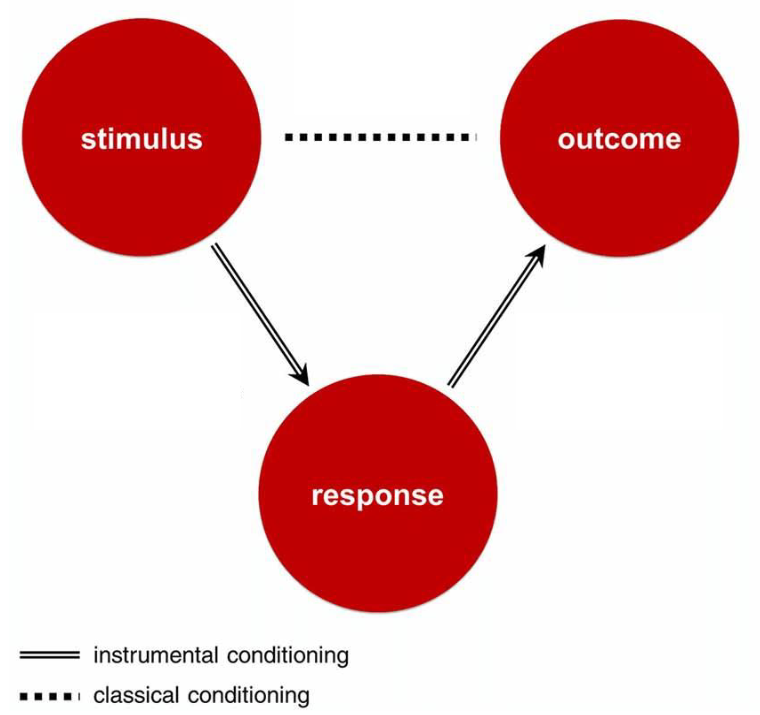
\includegraphics[width=0.35\linewidth]{./img/learning_systems.png}
        \caption{Learning systems relationship}
    \end{figure}
\end{remark}



\section{Learning at the neuronal level}

\begin{description}
    \item[Plasticity]
        Learning and experience change the connections of a neural system.

    \item[Short-term change]
        Functional physiological change that modifies the effectiveness of existing synaptic connections (i.e. amount of neurotransmitters).
        Lasts from seconds up to hours.

    \item[Long-term change]
        Structural change that leads to anatomical alterations such as pruning or growth of synapses.
        Lasts days and can cause further short-term changes.
\end{description}

\begin{remark}
    Neuronal changes follow a "use it or lose it" policy.
    Only useful changes will last.
\end{remark}

\begin{example}[Phantom limb pain]
    In amputees, the area of the brain responsible for the missing part of the body is overrun by the neighboring section.
    In the case of an arm, the area responsible for the face might "conquer" what once was the area of the arm.
\end{example}



\section{Pavlovian learning}
\marginnote{Pavlovian learning}

Form of prediction learning that aims to learn stimulus-outcome associations:
\begin{itemize}
    \item When a reinforcer is likely to occur.
    \item Which stimuli tend to precede a reinforcer.
\end{itemize}
This allows the animal to emit a response in anticipation of a reinforcer.

Pavlovian learning works as follows:\\
\begin{minipage}{0.58\linewidth}
    \begin{enumerate}[label=\alph*.]
        \item A stimulus that has no meaning to the animal will result in \ac{nr}.
        \item An \ac{us} (i.e. a reinforcer) generates an \ac{ur}.
        \item Learning happens when a reinforcer is paired with a non-relevant stimulus.
        \item The learned \ac{cs} generates a \ac{cr}.
    \end{enumerate}
\end{minipage}
\begin{minipage}{0.4\linewidth}
    \raggedleft
    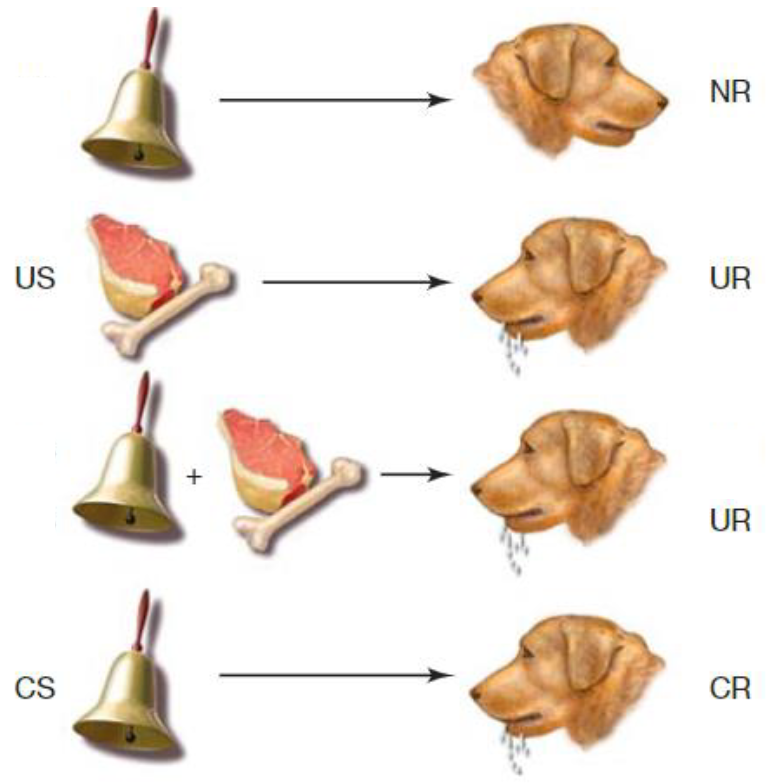
\includegraphics[width=0.9\linewidth]{./img/pavlovian_example.png}
\end{minipage}\\

An outcome can be:
\begin{descriptionlist}
    \item[Appetitive] Something considered positive.
    \item[Aversive] Something considered negative.
\end{descriptionlist}

The learned \acl{cr} can be:
\begin{descriptionlist}
    \item[Behavioral] Associated to the startle response (i.e. reflex in response to a sudden stimulus).
    \item[Physiological] Associated to the autonomic system.
    \item[Change in subjective response] 
\end{descriptionlist}

\begin{remark}
    Pavlovian learning has its foundations in behaviorism: the brain starts as a blank slate and only observable behaviors can be studied.
\end{remark}


\subsection{Types of reinforcement}

There are two types of learning:
\begin{descriptionlist}
    \item[Continuous reinforcement] \marginnote{Continuous reinforcement}
        The \acl{cs} is reinforced every time the \acl{us} occurs.
        \begin{remark}
            More effective to teach a new association.
        \end{remark}

    \item[Partial reinforcement] \marginnote{Partial reinforcement}
        The \acl{cs} is not always reinforced.
        \begin{remark}
            Learning is slower but the \acl{cr} is more resistant to extinction.
        \end{remark}
\end{descriptionlist}


\subsection{Learning flexibility}

\begin{description}
    \item[Acquisition] \marginnote{Acquisition}
        The probability of occurrence of a \acl{cr} increases if the \acl{cs} is presented with the \acl{us}.
        
    \item[Extinction] \marginnote{Extinction}
        The probability of occurrence of a \acl{cr} decreases if the \acl{cs} is presented alone.
\end{description}

\begin{remark}
    Extinction does not imply forgetting.
    After an association between \ac{cs} and \ac{us} is made, 
    extinction consists of creating a second association with inhibitory effects that overrides the existing association.

    The extinct association can return in the future
    (this is more evident when the context is the same as the acquisition phase).
\end{remark}

\begin{figure}[H]
    \centering
    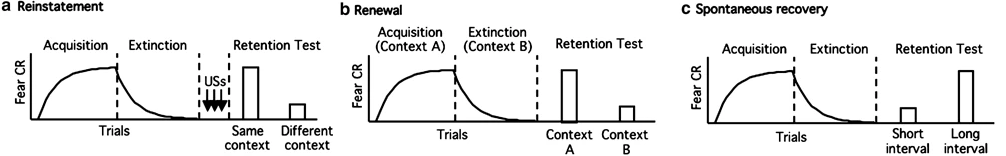
\includegraphics[width=\linewidth]{./img/pavlovian_extinction.png}
    \caption{Example of acquisition, extinction, and \ac{cr} return}
\end{figure}

\begin{description}
    \item[Generalization] \marginnote{Generalization} 
        A new stimulus that is similar to a learned \acl{cs} can elicit a \acl{cr}.
\end{description}



\section{Instrumental learning}
\marginnote{Instrumental learning}

Form of control learning that aims to learn action-outcome associations:
\begin{itemize}
    \item When a reinforcer is likely to occur.
    \item Which actions bring to those reinforcers.
\end{itemize}
This allows the animal to act in anticipation of a reinforcer.

Depending on the outcome, the effect varies:
\begin{descriptionlist}
    \item[Positive reinforcement] \marginnote{Positive reinforcement}
        Delivering an appetitive outcome to an action increases the probability of emitting it.

    \item[Positive punishment] \marginnote{Positive punishment}
        Delivering an aversive outcome to an action decreases the probability of emitting it.
    
    \item[Negative reinforcement] \marginnote{Negative reinforcement}
        Omitting an aversive outcome to an action increases the probability of emitting it.
    
    \item[Negative punishment] \marginnote{Negative punishment}
        Omitting an appetitive outcome to an action decreases the probability of emitting it.
\end{descriptionlist}

\begin{table}[H]
    \centering
    \begin{tabular}{r|cc}
        \toprule
                            & \textbf{Delivery}                         & \textbf{Omission} \\
        \midrule
        \textbf{Appetitive} & Positive reinforcement (\texttt{+prob})   & Negative punishment (\texttt{-prob}) \\
        \textbf{Aversive}   & Positive punishment (\texttt{-prob})      & Negative reinforcement (\texttt{+prob}) \\
        \bottomrule
    \end{tabular}
    \caption{Summary of the possible effects}
\end{table}


\subsection{Types of schedule}

There are two types of learning:
\begin{descriptionlist}
    \item[Continuous schedule] \marginnote{Continuous schedule}
        The desired action is followed by the outcome every time.
        \begin{remark}
            More effective to teach a new association.
        \end{remark}

    \item[Partial schedule] \marginnote{Partial schedule}
        The desired action is not always followed by the outcome.
        \begin{remark}
            Learning is slower but the response is more resistant to extinction.
        \end{remark}

        There are four types of partial schedules:
        \begin{descriptionlist}
            \item[Fixed-ratio] 
                Outcome available after a specific number of responses.

                This results in a high and steady rate of response, with a brief pause after the outcome is delivered.


            \item[Variable-ratio] 
                Outcome available after an unpredictable number of responses.

                This results in a high and steady rate of response.


            \item[Fixed-interval] 
                Outcome available after a specific interval of time.

                This results in a high rate of response near the end of the interval and a slowdown after the outcome is delivered.


            \item[Variable-interval] 
                Outcome available after an unpredictable interval of time.

                This results in a slow and steady rate of response.
        \end{descriptionlist}
\end{descriptionlist}
    \chapter{Pavlovian learning}


Form of prediction learning that aims to learn stimulus-outcome associations:
\begin{itemize}
    \item When a reinforcer is likely to occur.
    \item Which stimuli tend to precede a reinforcer.
\end{itemize}
This allows the animal to emit a response in anticipation of a reinforcer.

Pavlovian learning works as follows:\\
\begin{minipage}{0.58\linewidth}
    \begin{enumerate}[label=\alph*.]
        \item A stimulus that has no meaning to the animal will result in \ac{nr}.
        \item An \ac{us} (i.e. a reinforcer) generates an \ac{ur}.
        \item Learning happens when a reinforcer is paired with a non-relevant stimulus.
        \item The learned \ac{cs} generates a \ac{cr}.
    \end{enumerate}
\end{minipage}
\begin{minipage}{0.4\linewidth}
    \raggedleft
    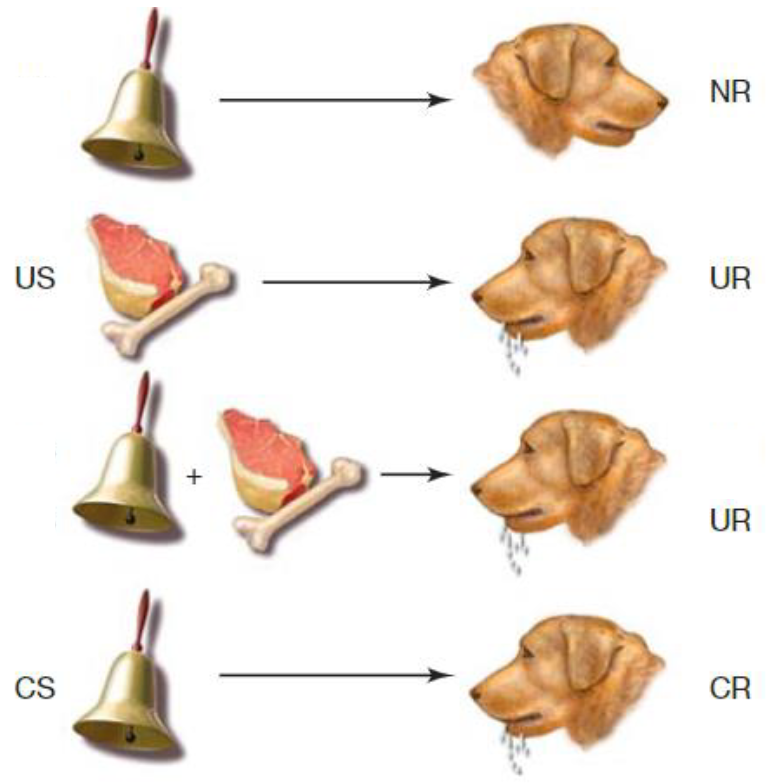
\includegraphics[width=0.9\linewidth]{./img/pavlovian_example.png}
\end{minipage}\\

An outcome can be:
\begin{descriptionlist}
    \item[Appetitive] Something considered positive.
    \item[Aversive] Something considered negative.
\end{descriptionlist}

The learned \acl{cr} can be:
\begin{descriptionlist}
    \item[Behavioral] Associated to the startle response (i.e. reflex in response to a sudden stimulus).
    \item[Physiological] Associated to the autonomic system.
    \item[Change in subjective response] 
\end{descriptionlist}

\begin{remark}
    Pavlovian learning has its foundations in behaviorism: the brain starts as a blank slate and only observable behaviors can be studied.
\end{remark}



\section{Types of reinforcement}

There are two types of learning:
\begin{descriptionlist}
    \item[Continuous reinforcement] \marginnote{Continuous reinforcement}
        The \acl{cs} is reinforced every time the \acl{us} occurs.
        \begin{remark}
            More effective to teach a new association.
        \end{remark}

    \item[Partial reinforcement] \marginnote{Partial reinforcement}
        The \acl{cs} is not always reinforced.
        \begin{remark}
            Learning is slower but the \acl{cr} is more resistant to extinction.
        \end{remark}
\end{descriptionlist}



\section{Learning flexibility}

\begin{description}
    \item[Acquisition] \marginnote{Acquisition}
        The probability of occurrence of a \acl{cr} increases if the \acl{cs} is presented with the \acl{us}.
        
    \item[Extinction] \marginnote{Extinction}
        The probability of occurrence of a \acl{cr} decreases if the \acl{cs} is presented alone.
\end{description}

\begin{remark}
    Extinction does not imply forgetting.
    After an association between \ac{cs} and \ac{us} is made, 
    extinction consists of creating a second association with inhibitory effects that overrides the existing association.

    The extinct association can return in the future
    (this is more evident when the context is the same as the acquisition phase).
\end{remark}

\begin{figure}[H]
    \centering
    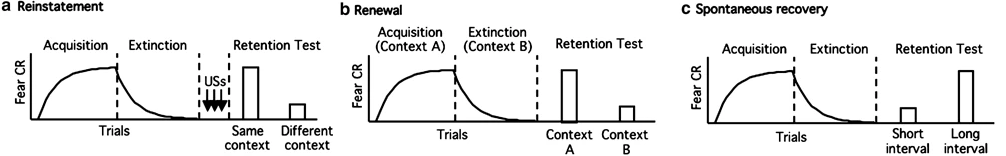
\includegraphics[width=0.95\linewidth]{./img/pavlovian_extinction.png}
    \caption{Example of acquisition, extinction, and \ac{cr} return}
\end{figure}

\begin{description}
    \item[Generalization] \marginnote{Generalization} 
        A new stimulus that is similar to a learned \acl{cs} can elicit a \acl{cr}.
\end{description}

\begin{casestudy}[Aplysia Californica] \phantom{}\\
    \begin{minipage}{0.8\linewidth}
        \begin{enumerate}
            \item Before conditioning, a stimulus to the siphon of an aplysia californica results in a weak withdrawal of the gill.
            \item During conditioning, a stimulus to the siphon is paired with a shock to the tail which results in a large withdrawal of the gill.
            \item After conditioning, a stimulus to the siphon alone results in a large withdrawal response.
        \end{enumerate}
    \end{minipage}
    \begin{minipage}{0.18\linewidth}
        \centering
        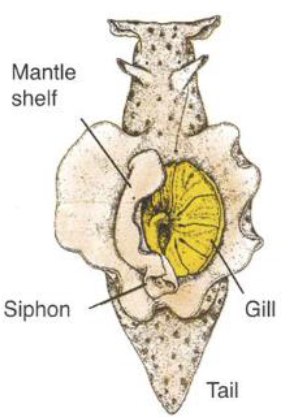
\includegraphics[width=\linewidth]{./img/aplysia.png}
    \end{minipage}

    \begin{figure}[H]
        \centering
        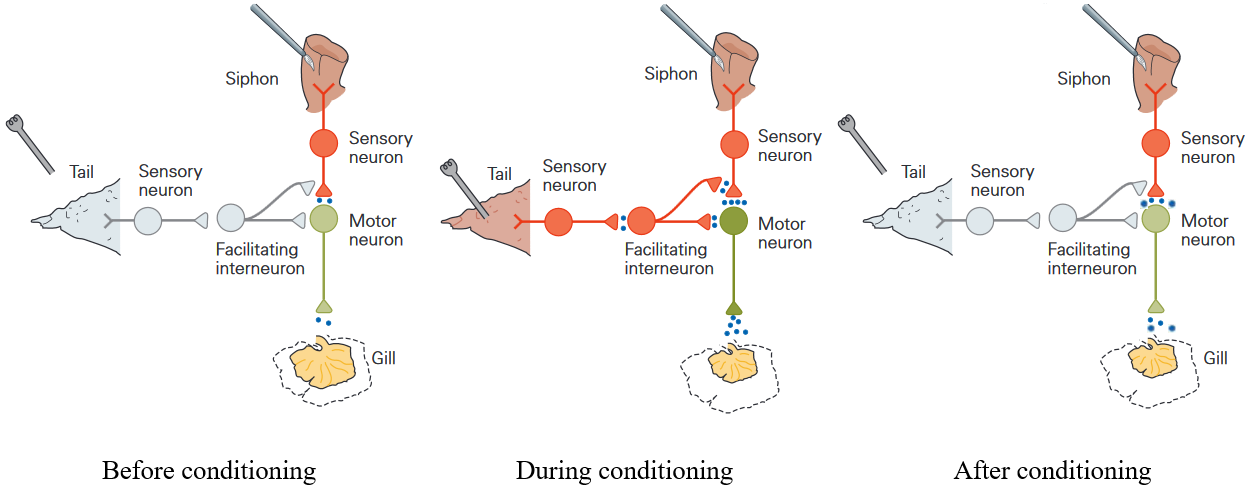
\includegraphics[width=0.85\linewidth]{./img/gill_pavlovian.png}
        \caption{Conditioning process}
    \end{figure}

    The learned response lasts for days.
    It can be observed that without training, the response disappears faster.

    \begin{figure}[H]
        \centering
        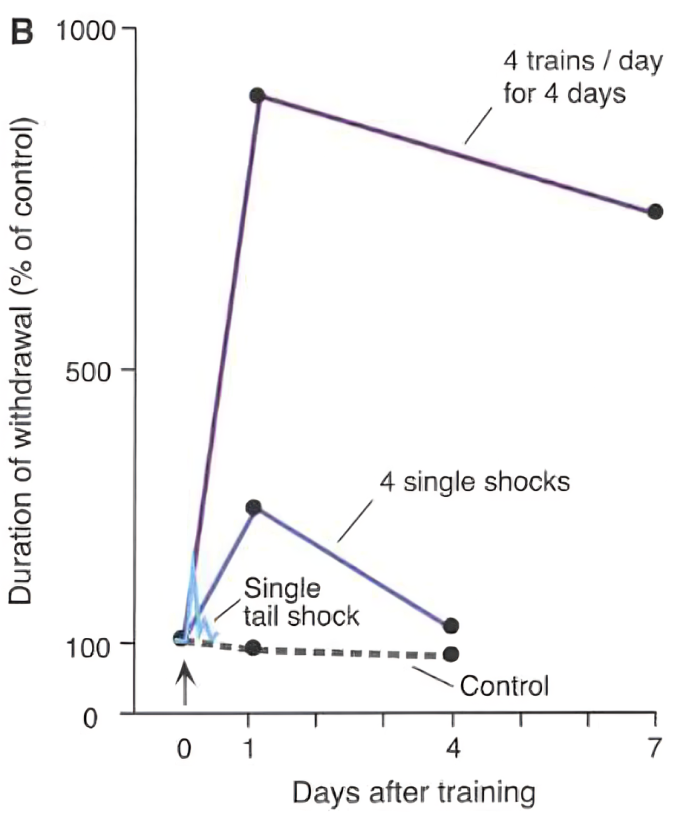
\includegraphics[width=0.3\linewidth]{./img/gill_pavlovian_graph.png}
        \caption{Withdrawal response decay}
    \end{figure}
\end{casestudy}

\begin{remark} \marginnote{Amygdala in Pavlovian learning}
    In mammals, aversive Pavlovian conditioning involves the amygdala.
    The \ac{cs} and \ac{us} are relayed from the thalamus and the cerebral cortex to the amygdala, 
    which in turn connects to various motor responses such as:
    \begin{descriptionlist}
        \item[Central gray region (CG)] Controls the freezing behavior.
        \item[Lateral hypothalamus (LH)] Controls autonomic responses.
        \item[Paraventricular hypothalamus (PVN)] Controls stress hormones.
    \end{descriptionlist}

    \begin{figure}[H]
        \centering
        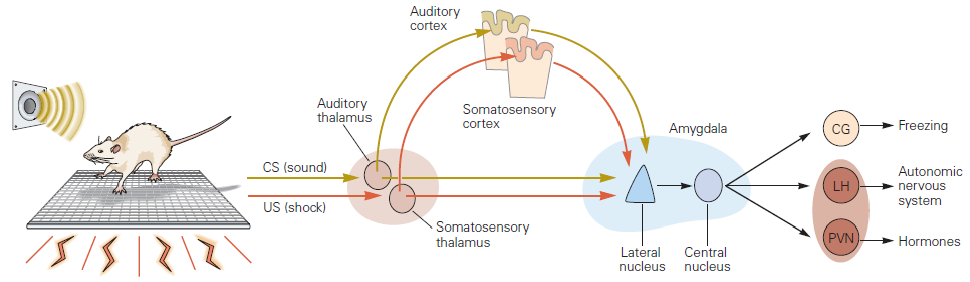
\includegraphics[width=0.9\linewidth]{./img/amygdala_pavlovian.png}
        \caption{Neural circuits during aversive conditioning}
    \end{figure}
\end{remark}



\section{Memory}
\marginnote{Memory}

Memory is vulnerable to alteration.
Once reactivated, the subsequent reconsolidation phase might store a modified version of the memory.

\begin{figure}[H]
    \centering
    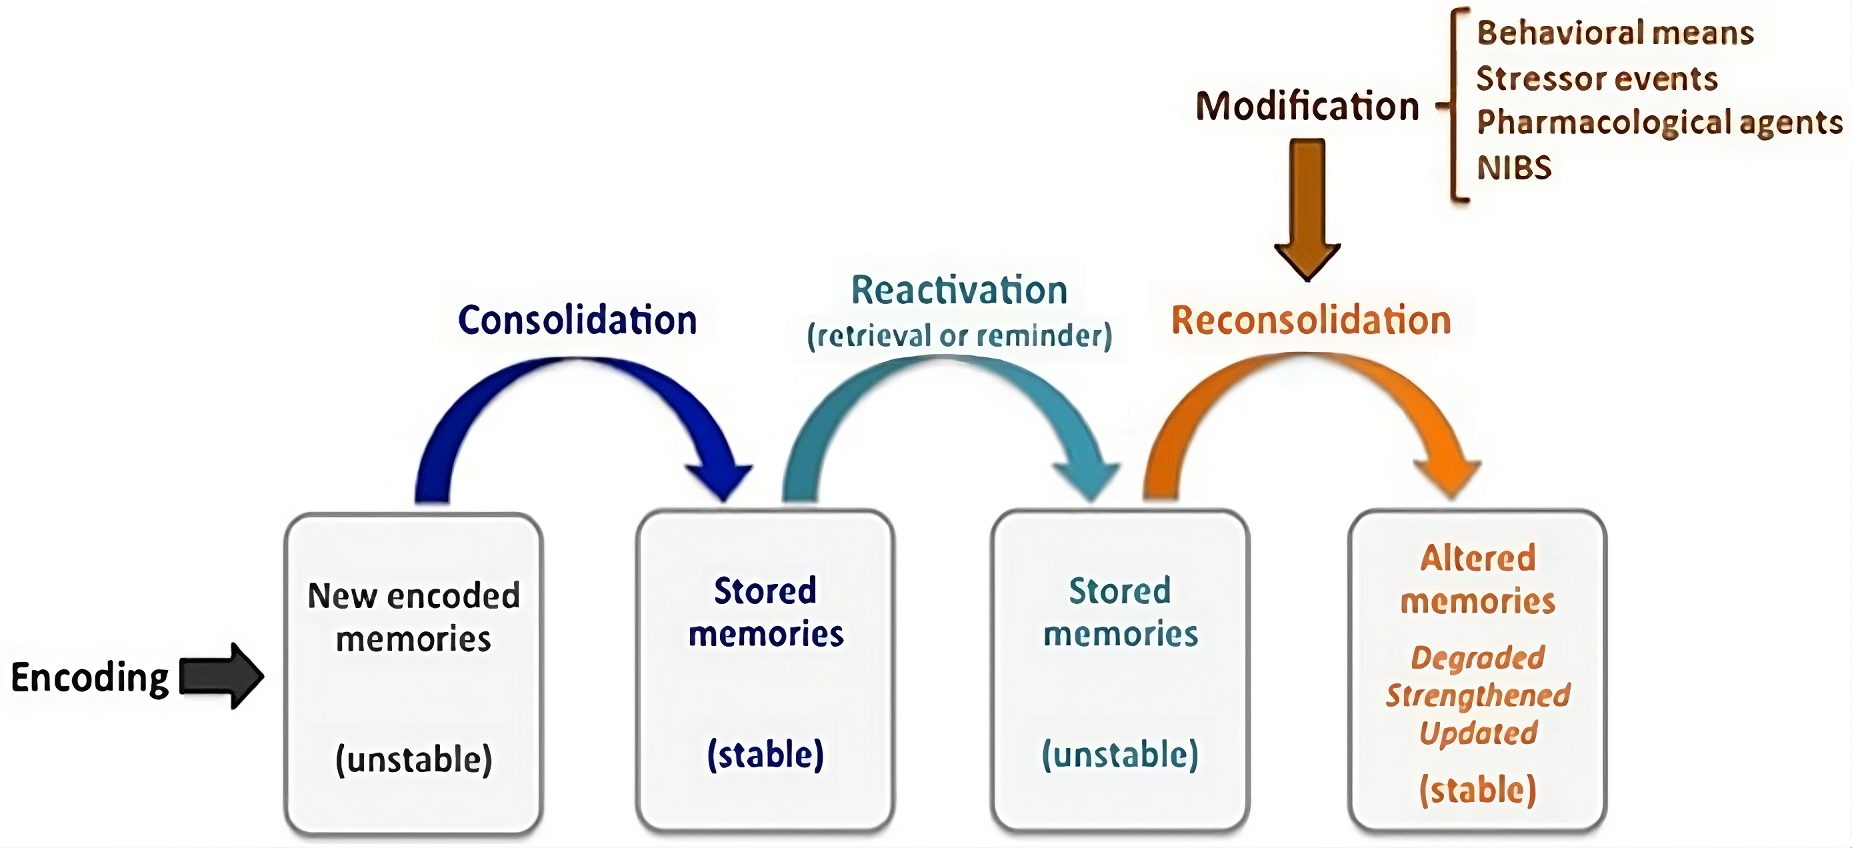
\includegraphics[width=0.6\linewidth]{./img/memory.png}
    \caption{Memory flow}
\end{figure}

\begin{remark}
    This mechanism is useful against traumatic memories.
\end{remark}

\begin{remark}
    The amygdala is responsible for storing conditioned responses while the hippocampus recognizes conditioned stimuli.

    Patients with a damaged amygdala only recognize \ac{cs} but do not act with any \ac{cr}.
    On the other hand, a damaged hippocampus results in patients that present a \ac{cr} without recognizing the \ac{cs}.
\end{remark}

\begin{casestudy}[Reconsolidation disruption]
    Propranolol is a drug that disrupts amygdala-specific memory reconsolidation (i.e. the physiological response).
    A possible therapy to suppress a phobia is to trigger the fear memory and then administer propranolol to prevent its reconsolidation.
\end{casestudy}



\section{Learning preconditions}

\subsection{Contiguity}
\marginnote{Contiguity}

Closeness between the \acl{cs} and the \acl{us}.

\begin{remark}
    The closer in time the stimuli are presented, the more likely the association will be created.
\end{remark}

Depending on when the \ac{cs} and \ac{us} are presented, conditioning can be:
\begin{descriptionlist}
    \item[Delay conditioning] \marginnote{Delay conditioning}
        The \ac{cs} is extended through the interstimulus interval (ISI) (i.e. time between the start of the \ac{cs} and the \ac{us}).

    \item[Trace conditioning] \marginnote{Trace conditioning}
        There is a delay (trace interval) between the \ac{cs} end and the \ac{us} start.

        Learning requires more trials and might be impossible if the trace interval is too long as the mental representation of the \ac{cs} decays.

    \begin{figure}[H]
        \centering
        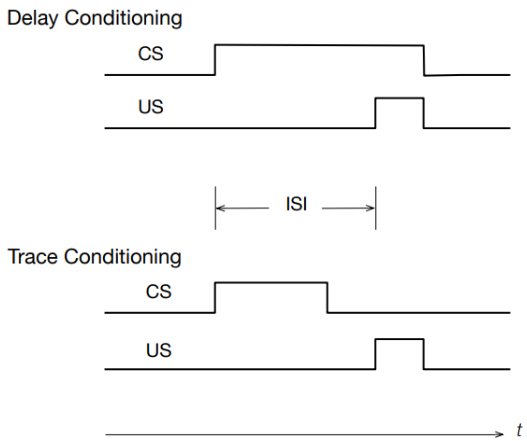
\includegraphics[width=0.45\linewidth]{./img/contiguity.png}
    \end{figure}
\end{descriptionlist}

\begin{casestudy}
    Two groups of rats were exposed to a 6 seconds tone (\ac{cs}) followed by food delivery (\ac{us}) with a delay of: 
    \begin{itemize}
        \item 6 seconds (red).
        \item 18 seconds (purple).
    \end{itemize}

    \begin{figure}[H]
        \centering
        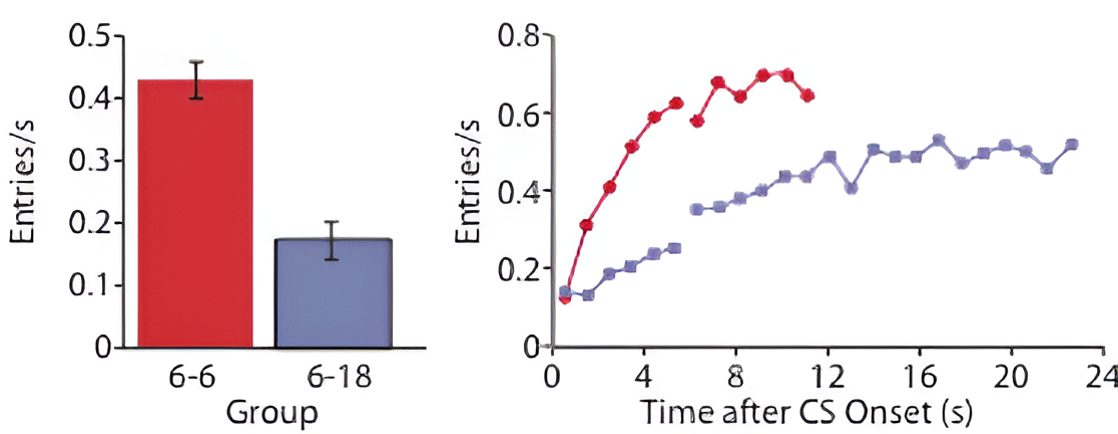
\includegraphics[width=0.55\linewidth]{./img/contiguity_rats.png}
        \caption{Number of entries (i.e. the rat checks the food tray) per second}
    \end{figure}
\end{casestudy}


\subsection{Contingency}
\marginnote{Contingency}

Causal relationship between the \acl{cs} and the \acl{us}.

\begin{remark}
    Learning happens when:
    \[ \prob{\text{\ac{us} with \ac{cs}}} > \prob{\text{\ac{us} with no \ac{cs}}} \]
    In other words, the \ac{cs} should provide information regarding the \ac{us}.
\end{remark}

\begin{figure}[H]
    \centering
    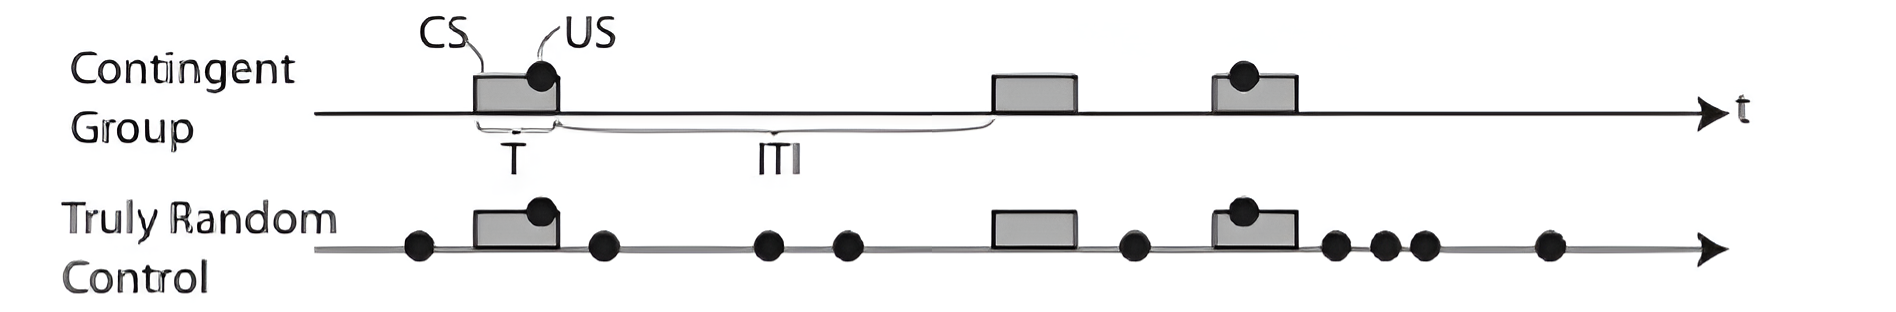
\includegraphics[width=0.6\linewidth]{./img/contingency.png}
    \caption{Example of contingent and random group}
\end{figure}

\begin{casestudy}
    Two groups of rats are exposed to a shock paired with a bell ring.
    Contiguity is the same but contingency differs.

    Only the group where the shock is more likely with the bell learns the association.

    \begin{figure}[H]
        \centering
        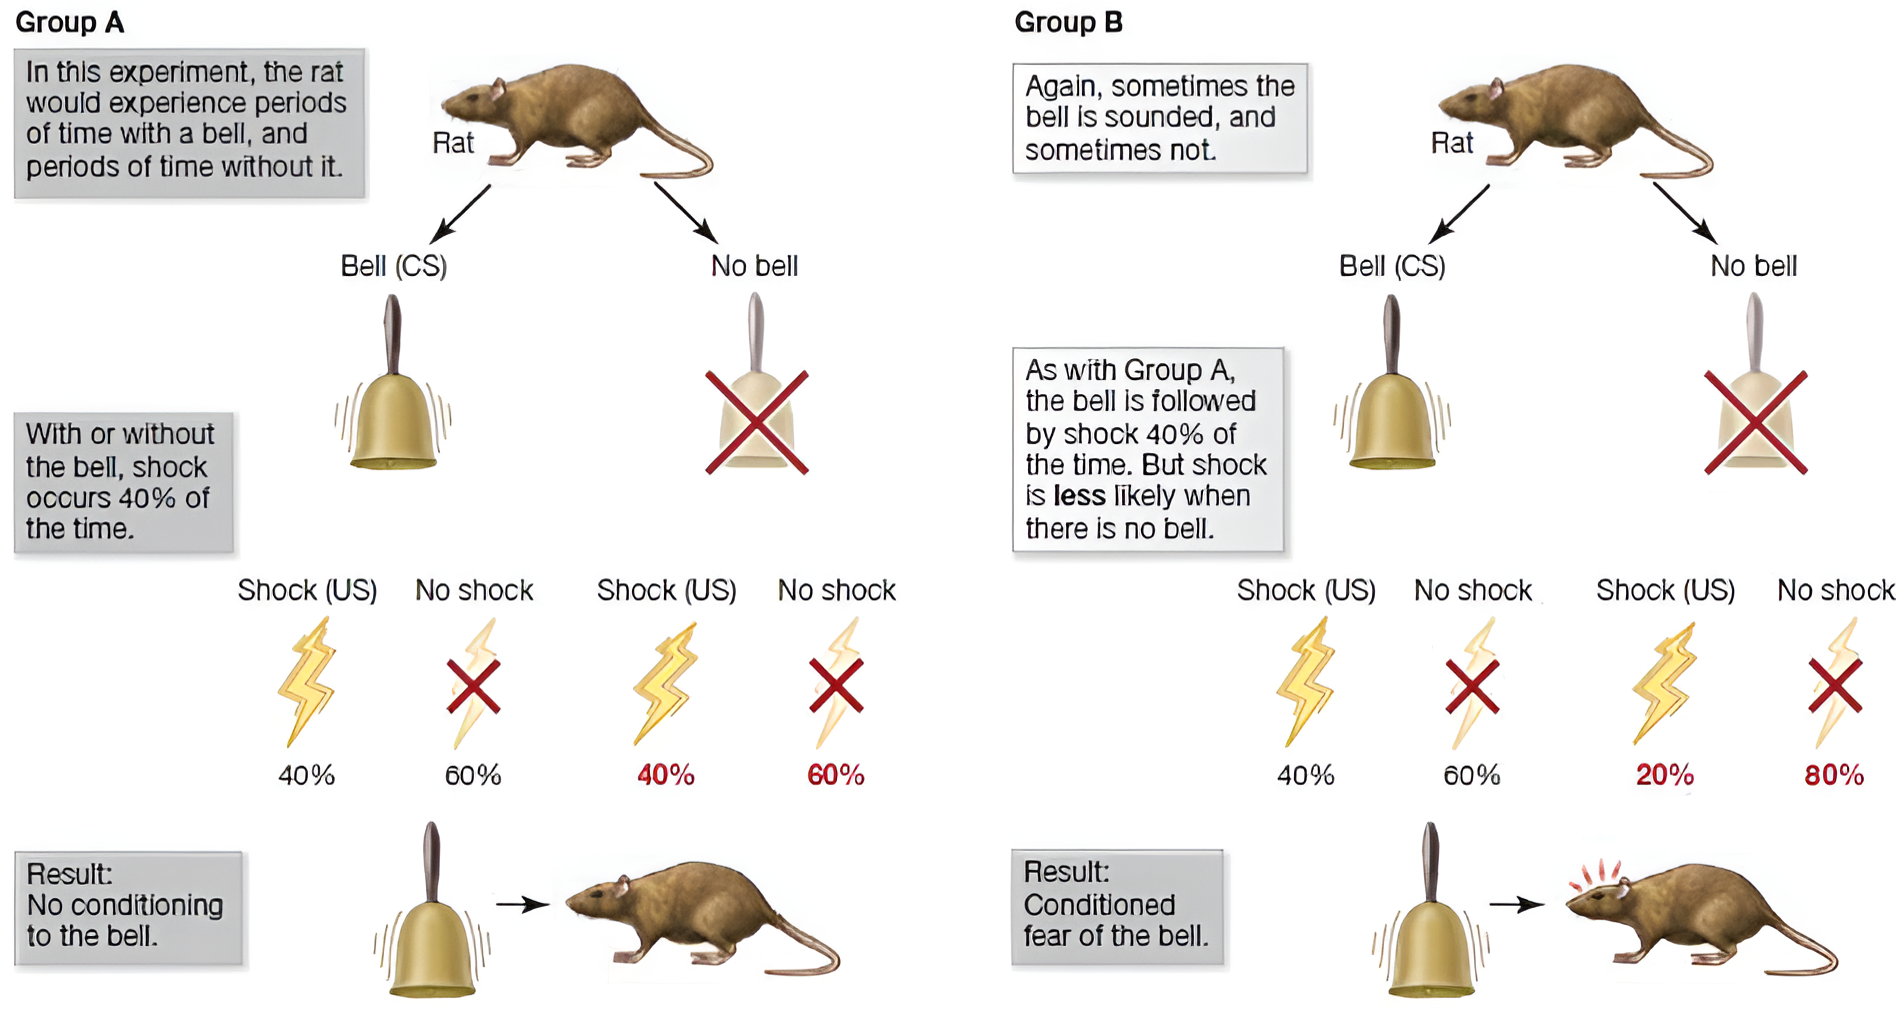
\includegraphics[width=0.8\linewidth]{./img/contingency_rats.png}
        \caption{Representation of the experiment}
    \end{figure}
\end{casestudy}


\subsection{Surprise}

\begin{description}
    \item[Prediction error] \marginnote{Prediction error}
        Quantitative discrepancy between the expected and experienced outcome.
\end{description}

\begin{remark}
    Learning happens when the outcome is different from what was expected.
\end{remark}

\begin{figure}[H]
    \centering
    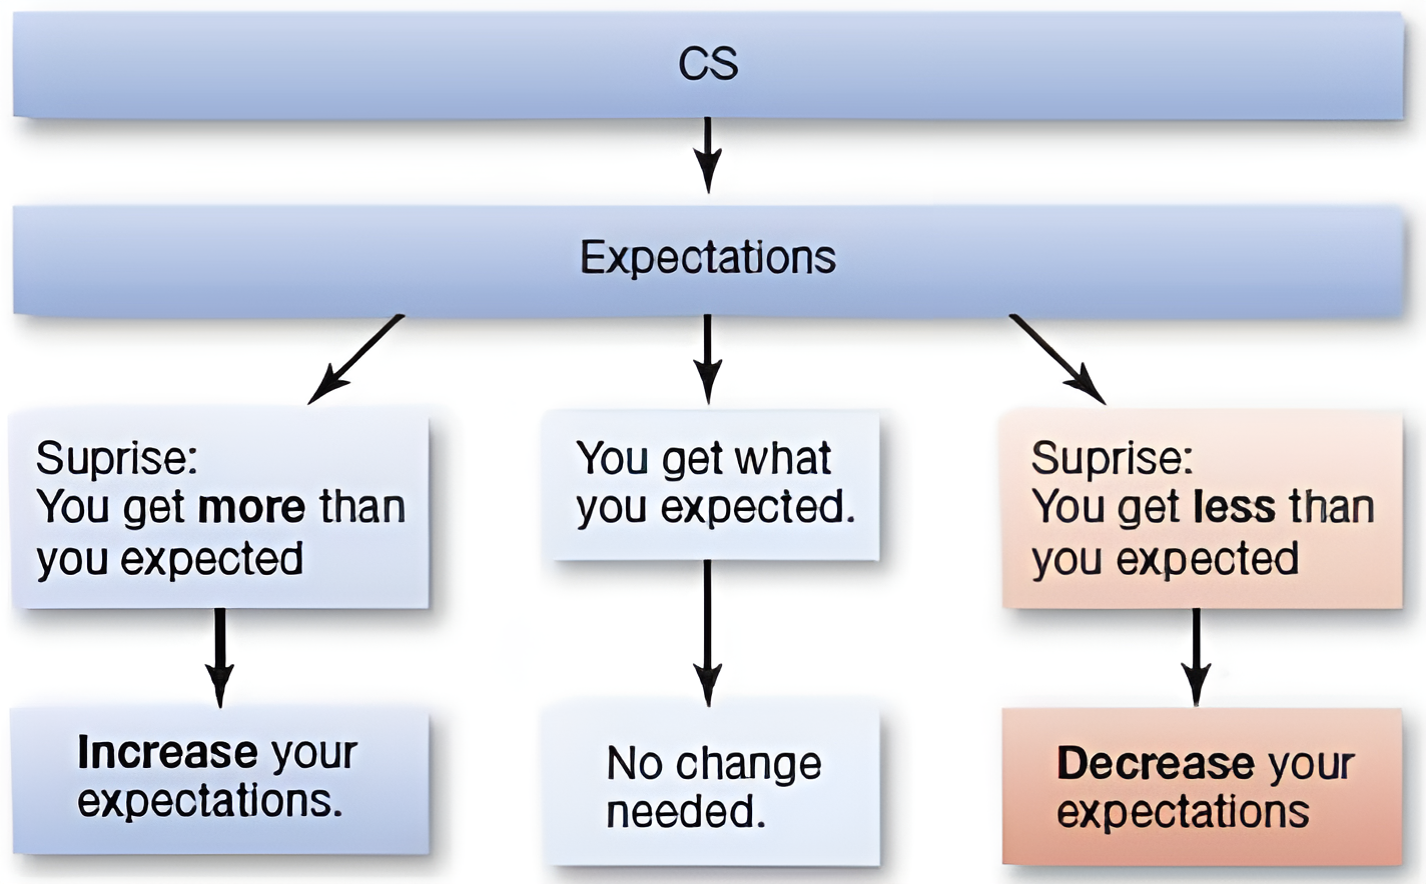
\includegraphics[width=0.4\linewidth]{./img/surprise.png}
    \caption{Learning outcome due to surprise}
\end{figure}

\begin{casestudy}[Blocking effect]
    \phantom{} \label{ex:blocking} \\
    \begin{minipage}{0.65\linewidth}
        \begin{enumerate}
            \item A rat is taught that a hissing sound (\ac{cs}) is paired with a sexually receptive mate (\ac{us}).
            \item A light is added together with the hissing sound.
            \item When only the light is presented, the rat does not provide a response.
        \end{enumerate}

        The light is not learned as a \ac{cs} as it does not provide any new information on the \ac{us}.
    \end{minipage}
    \begin{minipage}{0.35\linewidth}
        \begin{figure}[H]
            \centering
            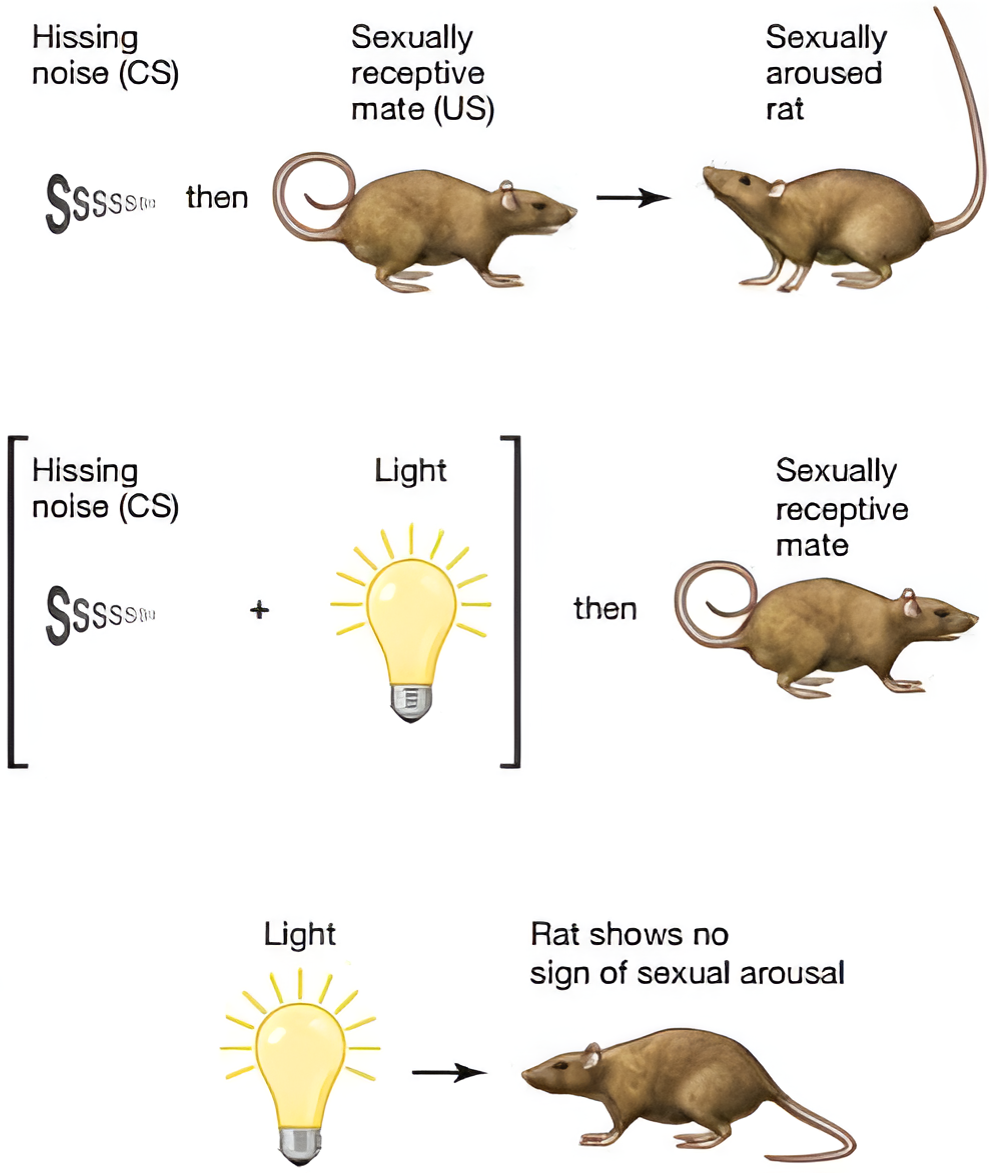
\includegraphics[width=\linewidth]{./img/surprise_rats.png}
        \end{figure}
    \end{minipage}
\end{casestudy}



\section{Computational model}


\subsection{Rescorla-Wagner model}
\marginnote{Rescorla-Wagner model}

Error-driven learning model where the change expectancy is proportional to the difference between predicted and actual outcome:
\[ \delta_{tr} = R_{tr} - V_{tr} \]
where:
\begin{itemize}
    \item $\delta_{tr}$ is the prediction error.
    \item $R_{tr} = \begin{cases}
            1 & \text{if the \ac{us} is delivered at trial $tr$} \\
            0 & \text{if the \ac{us} is omitted at trial $tr$}
        \end{cases}$.
    \item $V_{tr}$ is the association strength (i.e. expectancy of the \ac{us} or the expected value resulting from a given \ac{cs}) at trial $tr$.
\end{itemize}

Then, the expected value $V_{tr+1}$ is obtained as:
\[ V_{tr+1} = V_{tr} + \alpha \delta_{tr} \]
where $\alpha \in [0, 1]$ is the learning rate.

\begin{remark}
    A lower $\alpha$ is more suited for volatile environments.
\end{remark}

\begin{remark}
    The prediction error $\delta$ is:
    \begin{itemize}
        \item Positive during acquisition.
        \item Negative during extinction.
    \end{itemize}
    Moreover, the error is larger at the start of acquisition/extinction.
\end{remark}

\begin{remark}
    The Rescorla-Wagner model is able to capture the blocking effect (see \hyperref[ex:blocking]{Blocking example}) as
    the animal computes a single prediction error obtained as the combination of multiple stimuli.
\end{remark}

\begin{figure}[H]
    \centering
    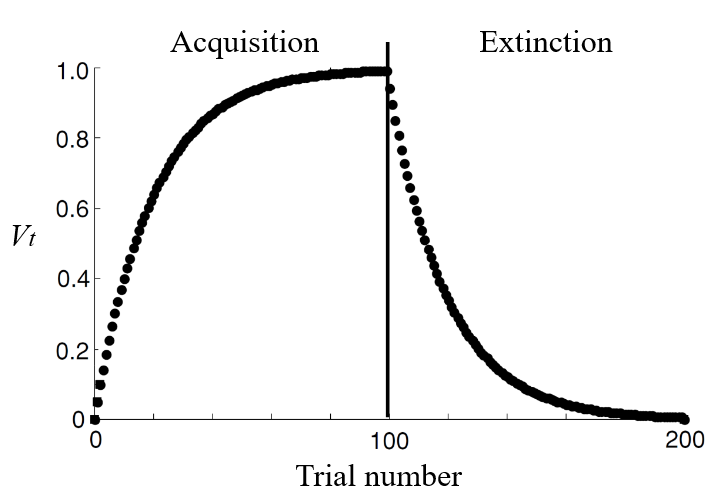
\includegraphics[width=0.4\linewidth]{./img/rescorla_wagner_curve.png}
    \caption{Acquisition and extinction in Pavlovian learning according to the Rescorla-Wagner model}
\end{figure}

\begin{remark}
    The Rescorla-Wagner model is a trial-level model that only considers the change from trial to trial
    without considering what happens within and between trials.
\end{remark}


\subsection{Temporal difference model}
\marginnote{Temporal difference model}

Real-time model based on time steps within a trial instead of monolithic trials.
At each time $t$ of a trial during which a \ac{cs} is presented,
the model computes a prediction of the total future reward that will be gained from time $t$ to the end of the trial.

The prediction error is computed as follows\footnote{\url{https://pubmed.ncbi.nlm.nih.gov/9054347/}}:
\begin{gather*}
    \delta_t = R_t + V_{t+1} - V_t \\
    V_{t+1} = V_t + \alpha \delta_t
\end{gather*}

\begin{itemize}
    \item At the beginning of learning, the \ac{cs} is presented at time $t_\text{\ac{cs}}$
        and $V_t = 0$ until the \ac{us} is delivered at time $t_\text{\ac{us}} > t_\text{\ac{cs}}$.
    \item On the next trial, $V_{t_\text{\ac{us}}} - V_{t_\text{\ac{us}} - 1}$ now generates a positive prediction error that updates $V_{t_\text{\ac{us}} - 1}$.
    \item On subsequent trials, $V_t$ is updated for each $t$ in between $t_\text{\ac{us}}$ back to $t_\text{\ac{cs}}$.
\end{itemize}

In other words, the value signal produced by the reward (\ac{us}) is transferred back to an event (\ac{cs}) that predicts the reward.

\begin{casestudy}[Second-order conditioning]
    Pairing a new \ac{cs} to an existing \ac{cs}.

    \begin{center}
        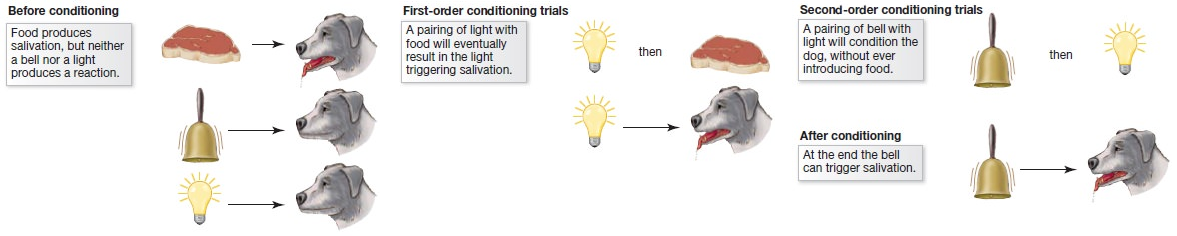
\includegraphics[width=0.95\linewidth]{./img/second_order_conditioning.png}
    \end{center}

    \begin{remark}
        The Rescorla-Wagner model is not capable of modeling second-order conditioning while 
        the temporal difference model is.
    \end{remark}
\end{casestudy}



\section{Reward prediction error hypothesis of dopamine}

There is strong evidence that the dopaminergic system is the major neural mechanism of reward and reinforcement.

\begin{description}
    \item[Response to unexpected rewards] \marginnote{Dopamine response to unexpected rewards}
        Dopaminergic neurons exhibit a strong phasic response in the presence of an unexpected reward.

        \begin{casestudy}[Monkey that touches food]
            Some food is put in a box with a hole to reach its content.
            In the absence of any other stimuli predicting the reward, 
            a monkey presents a high dopaminergic response when it touches the food.
            \begin{center}
                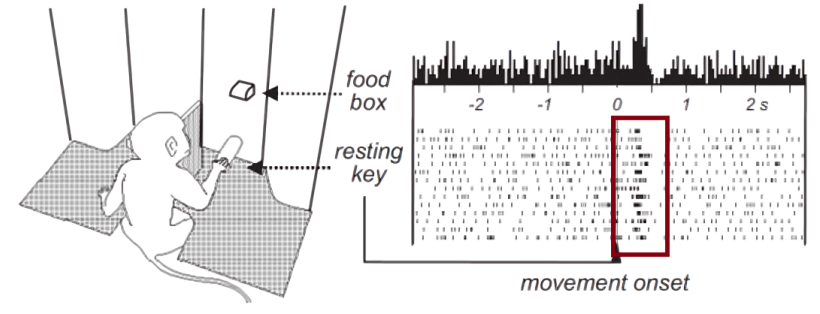
\includegraphics[width=0.55\linewidth]{./img/dopamine_monkey1.png}    
            \end{center}
        \end{casestudy}

    \item[Reward discrimination] \marginnote{Dopamine reward discrimination}
        Dopamine neurons respond differently depending on the actual presence of a reward.

        \begin{casestudy}[Monkey that touches food]
            The dopaminergic response of a monkey that touches an apple attached to a wire in a box is different 
            from the response of only touching the wire.
            \begin{center}
                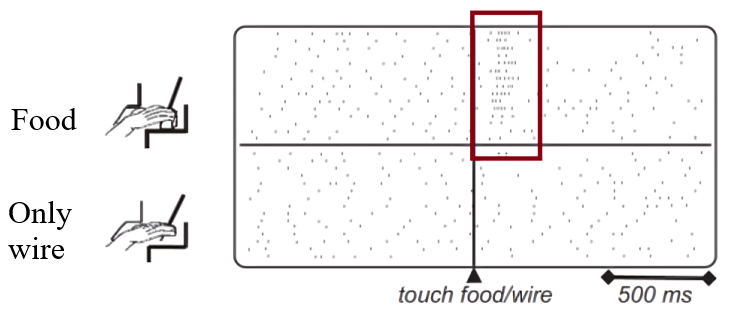
\includegraphics[width=0.5\linewidth]{./img/dopamine_monkey2.png}    
            \end{center}
        \end{casestudy}

    \item[Magnitude discrimination] \marginnote{Dopamine magnitude discrimination}
        Dopamine neurons respond differently depending on the amount of reward received.

        \begin{casestudy}[Monkey that drinks]
            By giving a monkey different amounts of fruit juice in a pseudorandom order,
            its dopaminergic response is stronger for the highest volume and weaker for the lowest volume.
            \begin{center}
                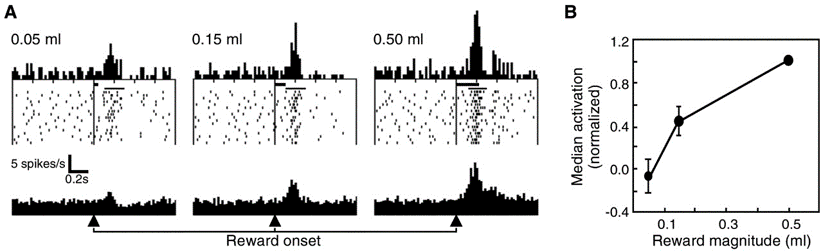
\includegraphics[width=0.7\linewidth]{./img/dopamine_monkey3.png}    
            \end{center}
        \end{casestudy}

        \begin{casestudy}[Monkey with juice and images]
            Using different \acp{cs}, it can be seen that the dopaminergic response differs based on the amount of reward.
            \begin{center}
                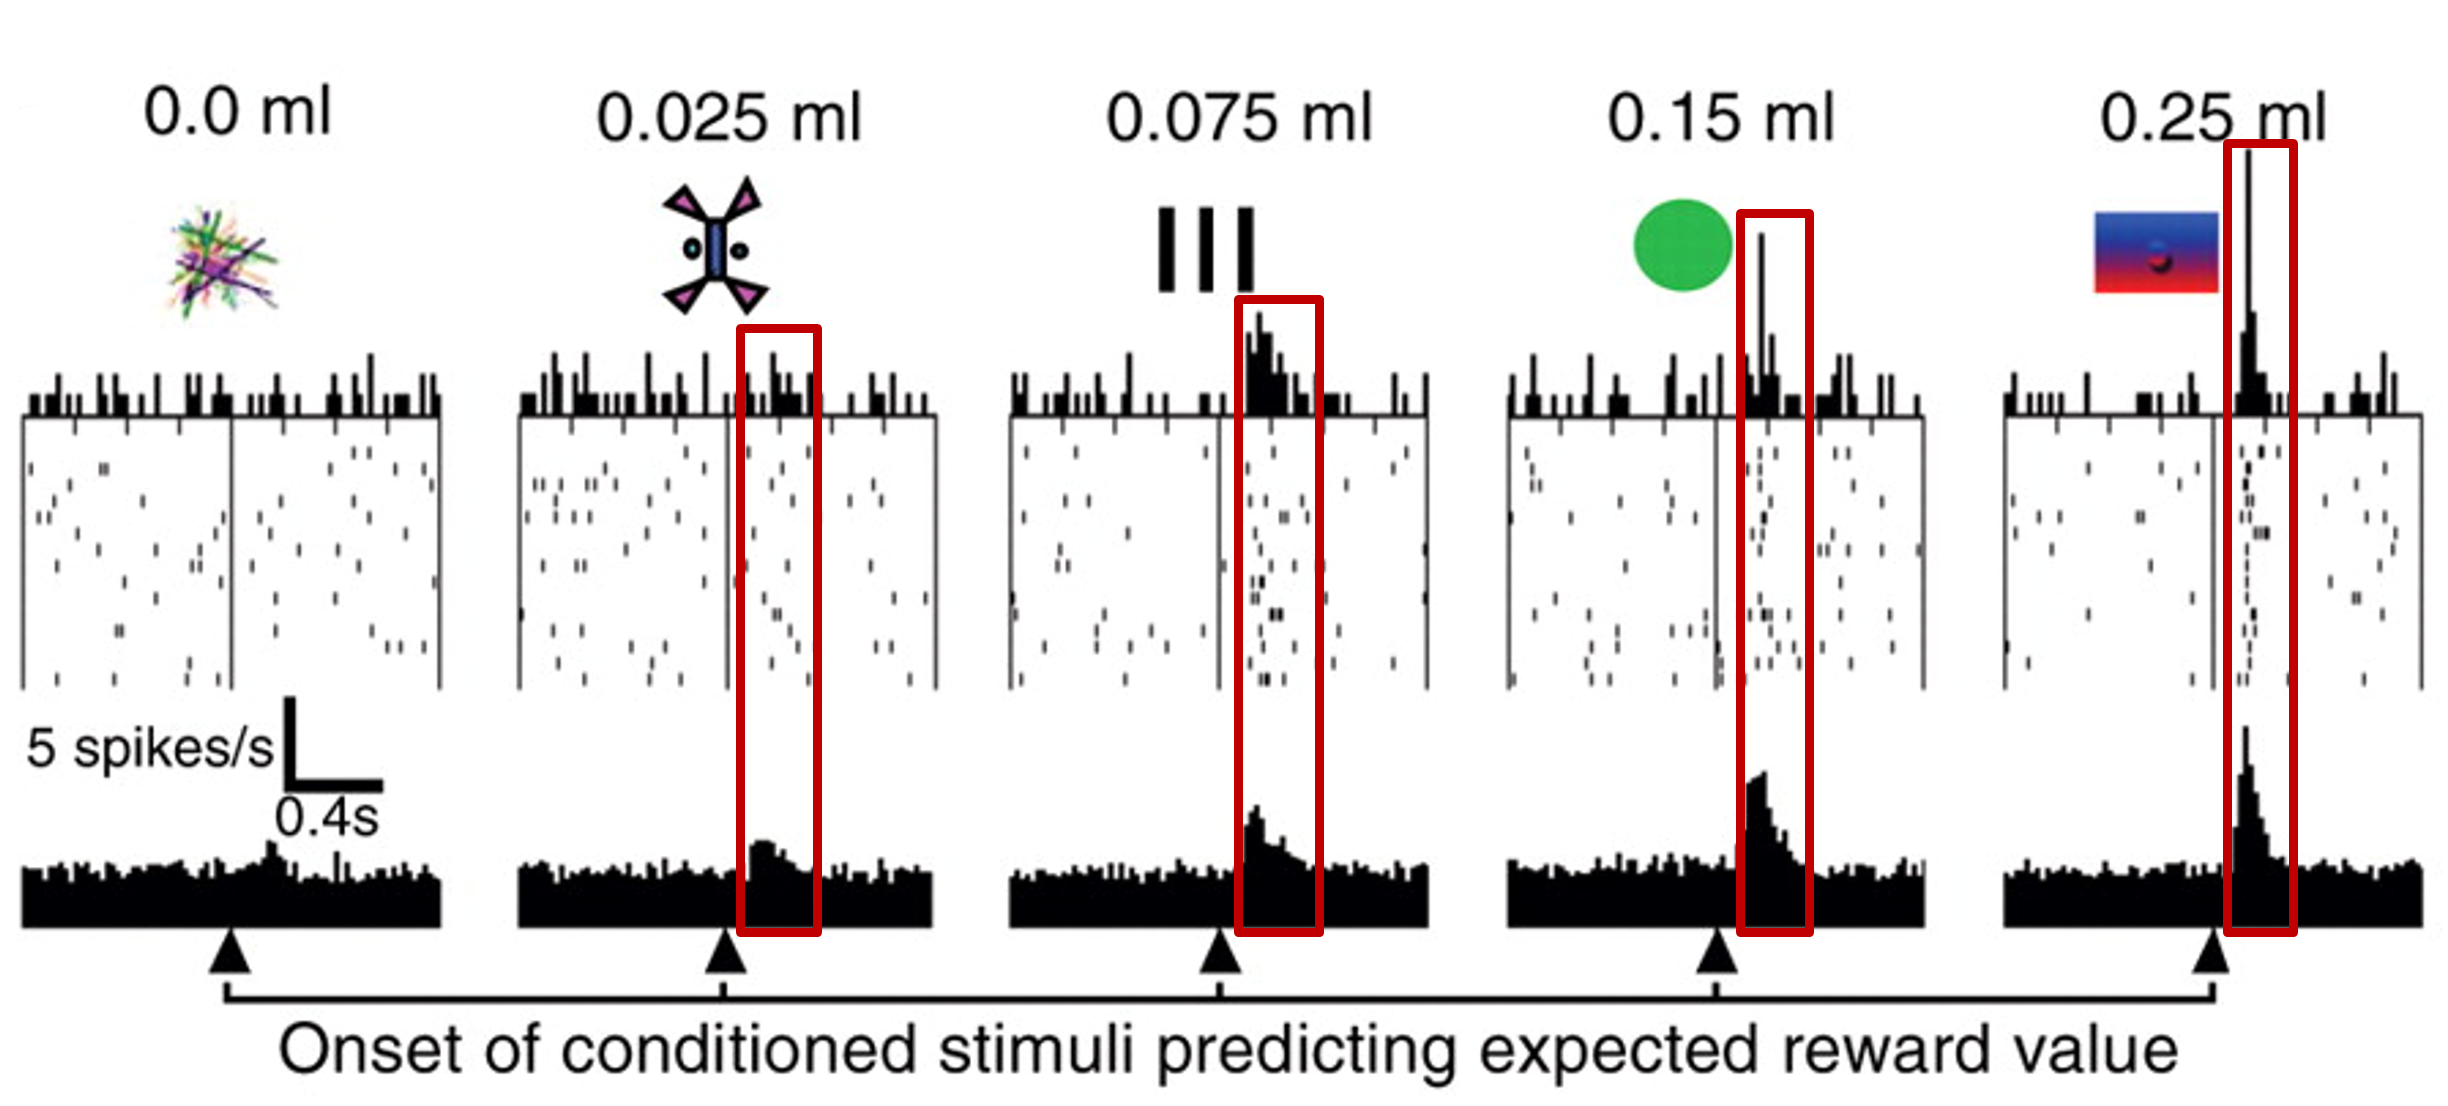
\includegraphics[width=0.55\linewidth]{./img/dopamine_expected.png}
            \end{center}
        \end{casestudy}

        \begin{casestudy}[Monkey with juice and images]
            After learning the association between a \ac{cs} and \ac{us} (middle graph), a change in the amount of the reward changes the dopaminergic response.
            \begin{center}
                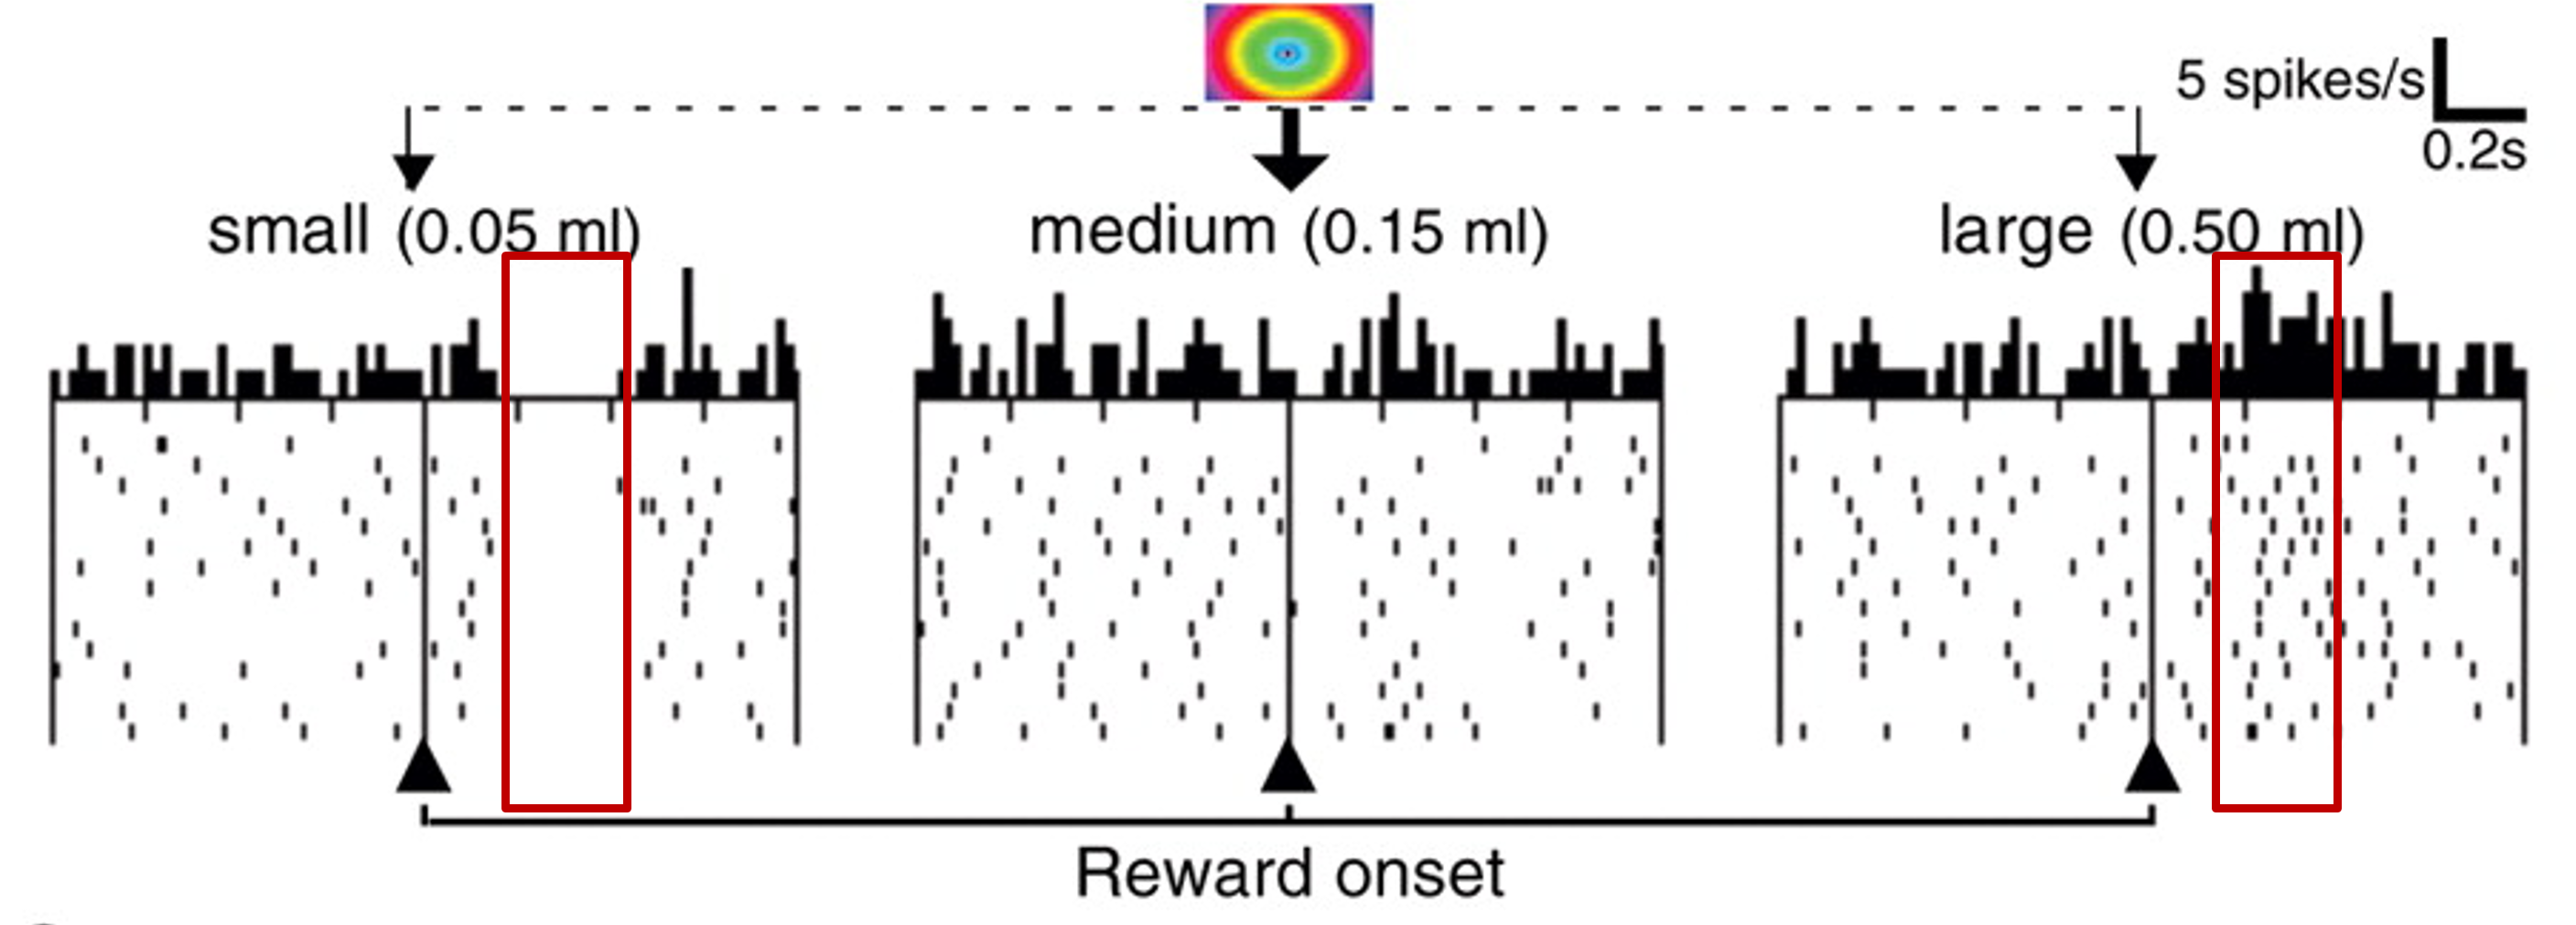
\includegraphics[width=0.6\linewidth]{./img/dopamine_expected2.png}
            \end{center}

            This behavior also involves the context (i.e. the \ac{cs} image that is shown).
            \begin{center}
                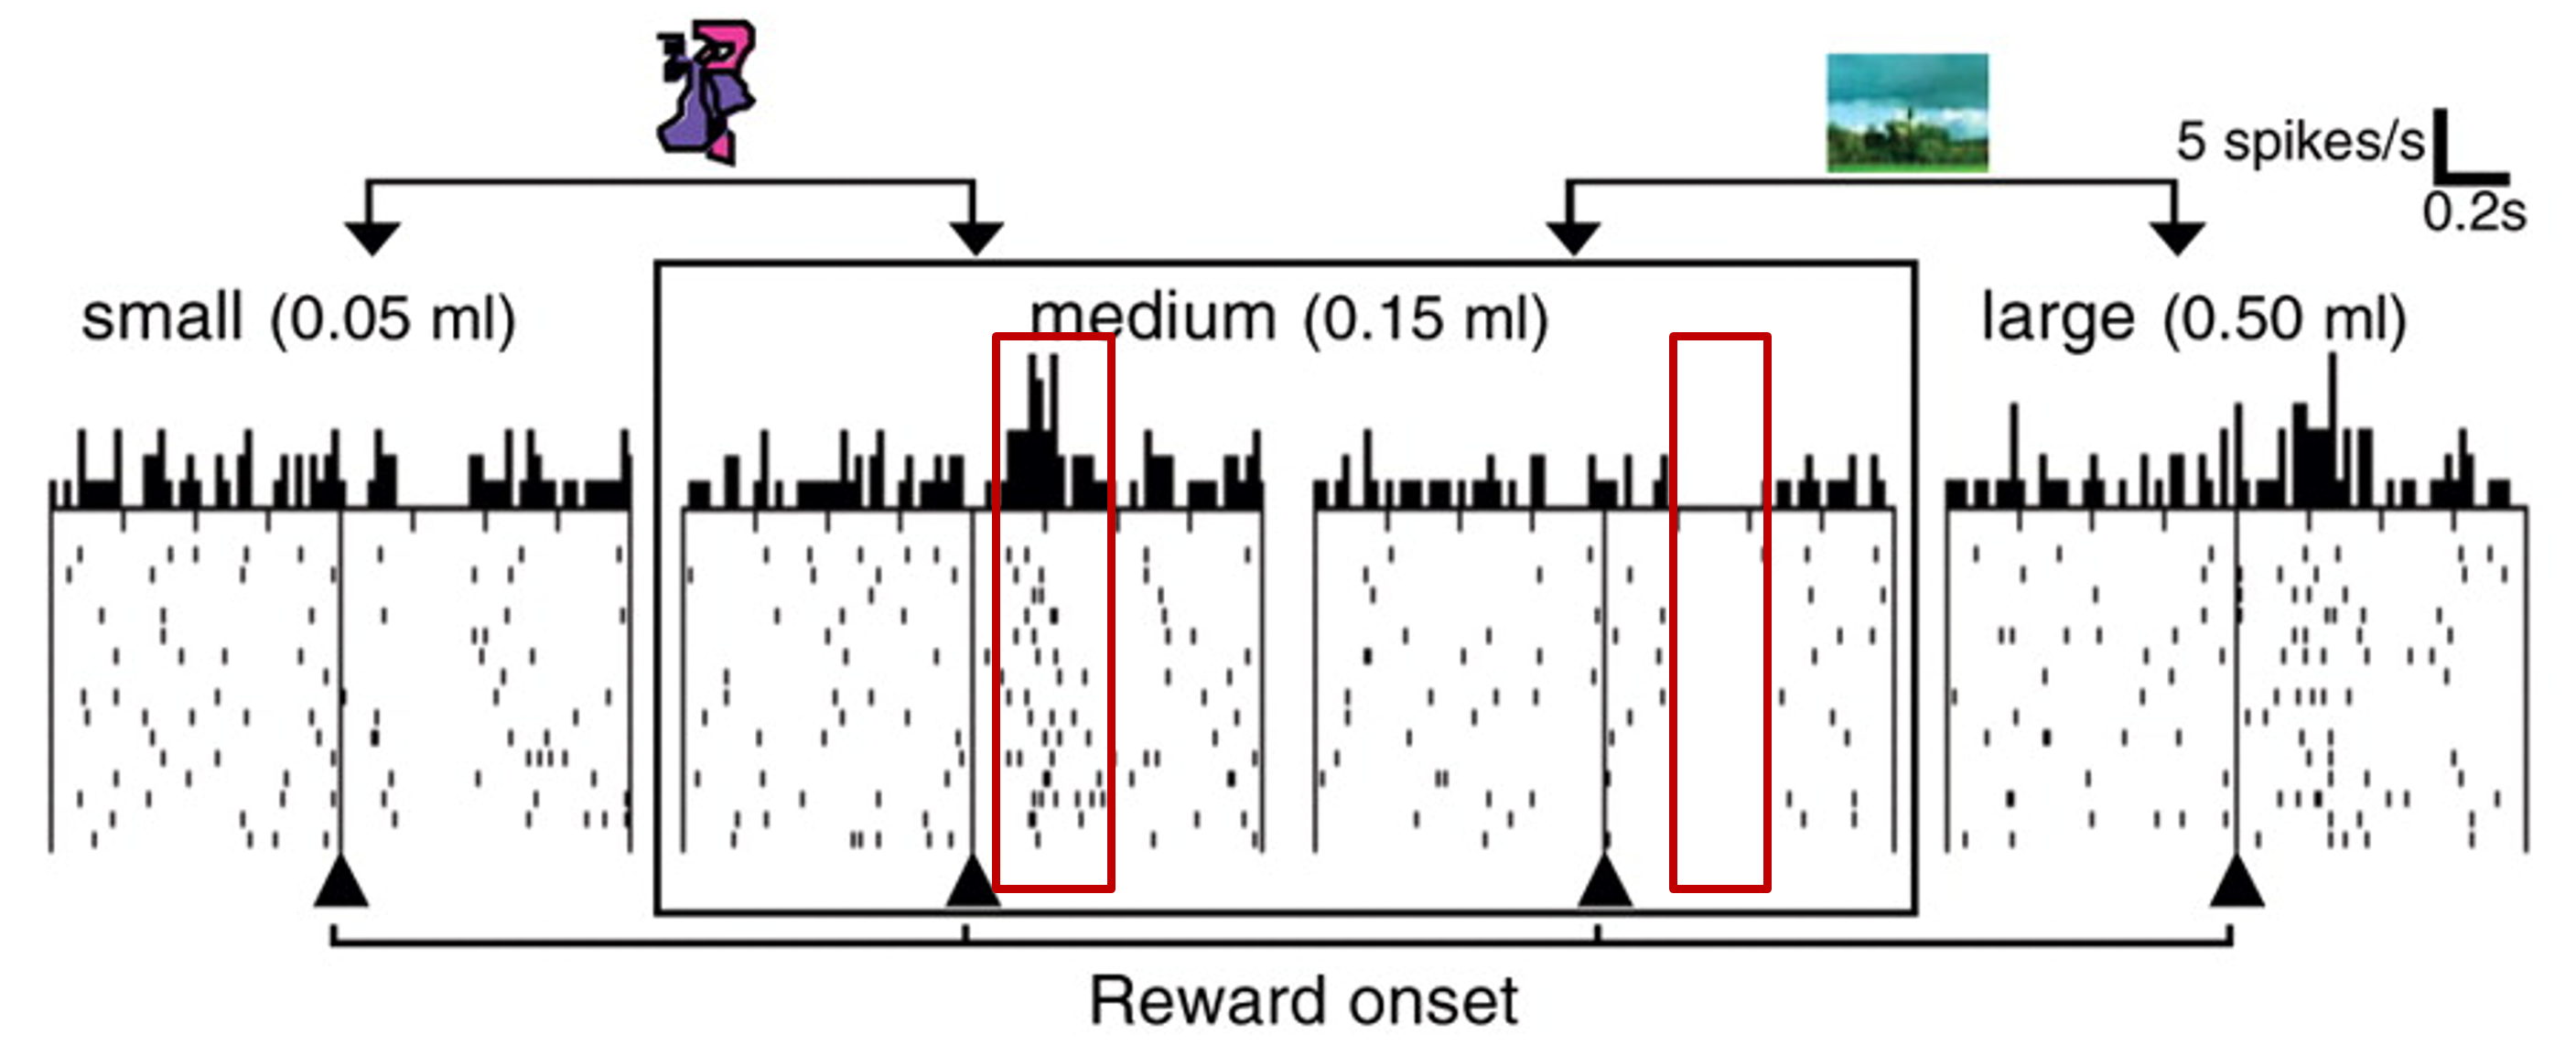
\includegraphics[width=0.6\linewidth]{./img/dopamine_expected3.png}
            \end{center}
        \end{casestudy}
\end{description}

\begin{remark}
    With the previous observations, it can be concluded that:
    \begin{itemize}
        \item Dopamine neurons increase their firing rate when the reward is unexpectedly delivered or better than expected.
        \item Dopamine neurons decrease their firing rate when the reward is unexpectedly omitted or worse than expected.
    \end{itemize}
\end{remark}

\begin{description}
    \item[Transfer to \ac{cs}] \marginnote{Dopamine transfer to \ac{cs}}
        \begin{itemize}
            \item Before training, an unexpected reward (\ac{us}) causes the dopamine neurons to increase firing (positive prediction error).
            \item After training, dopamine neurons firing is increased after the \ac{cs} but not following the reward (no prediction error).
            \item After training, dopamine neurons firing is increased after the \ac{cs} but is decreased if the reward is omitted (negative prediction error).
        \end{itemize}
        \begin{center}
            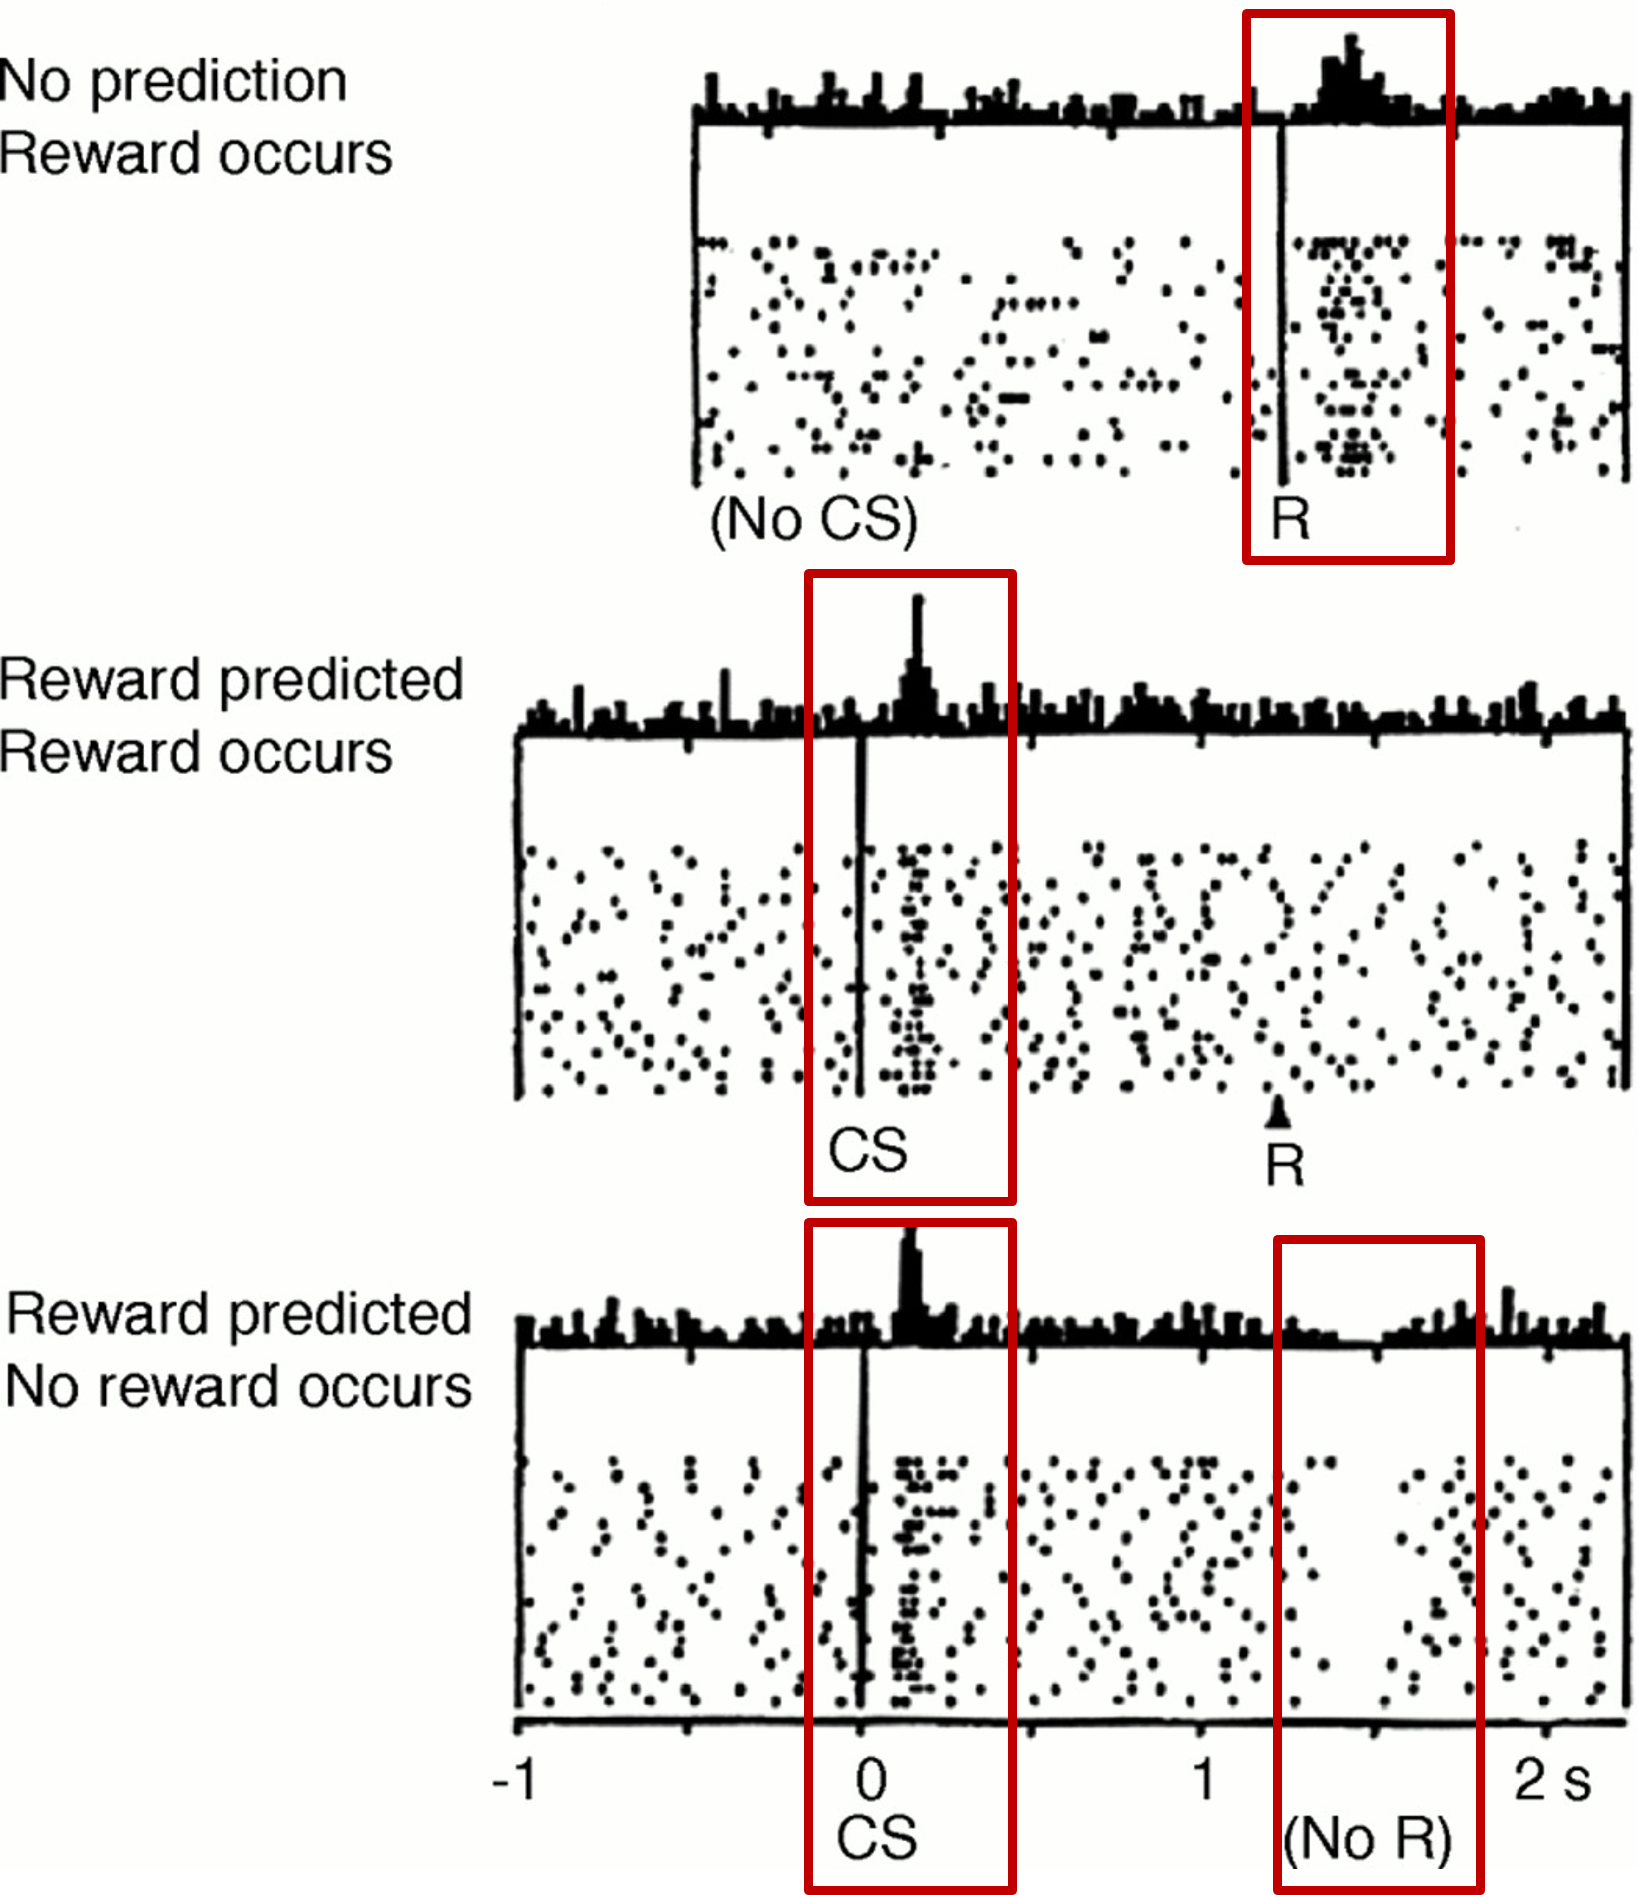
\includegraphics[width=0.4\linewidth]{./img/dopamine_transfer_cs.png}
        \end{center}

    \item[Response to blocking] \marginnote{Dopamine response to blocking}
        Dopaminergic response is in line with the blocking effect.

        \begin{casestudy}[Monkey with food and images]
            \phantom{}\\
            \begin{minipage}{0.7\linewidth}
                A monkey is taught to associate images with food.
                A new \ac{cs} alongside an existing \ac{cs} will not be learned.
            \end{minipage}
            \begin{minipage}{0.28\linewidth}
                \centering
                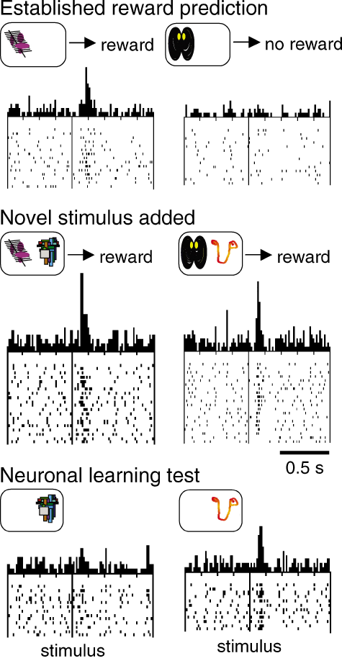
\includegraphics[width=\linewidth]{./img/dopamine_blocking.png}
            \end{minipage}
        \end{casestudy}

    \item[Probability encoding] \marginnote{Dopamine probability encoding}
        The phasic activation of dopamine neurons varies monotonically with the reward probability
        \begin{center}
            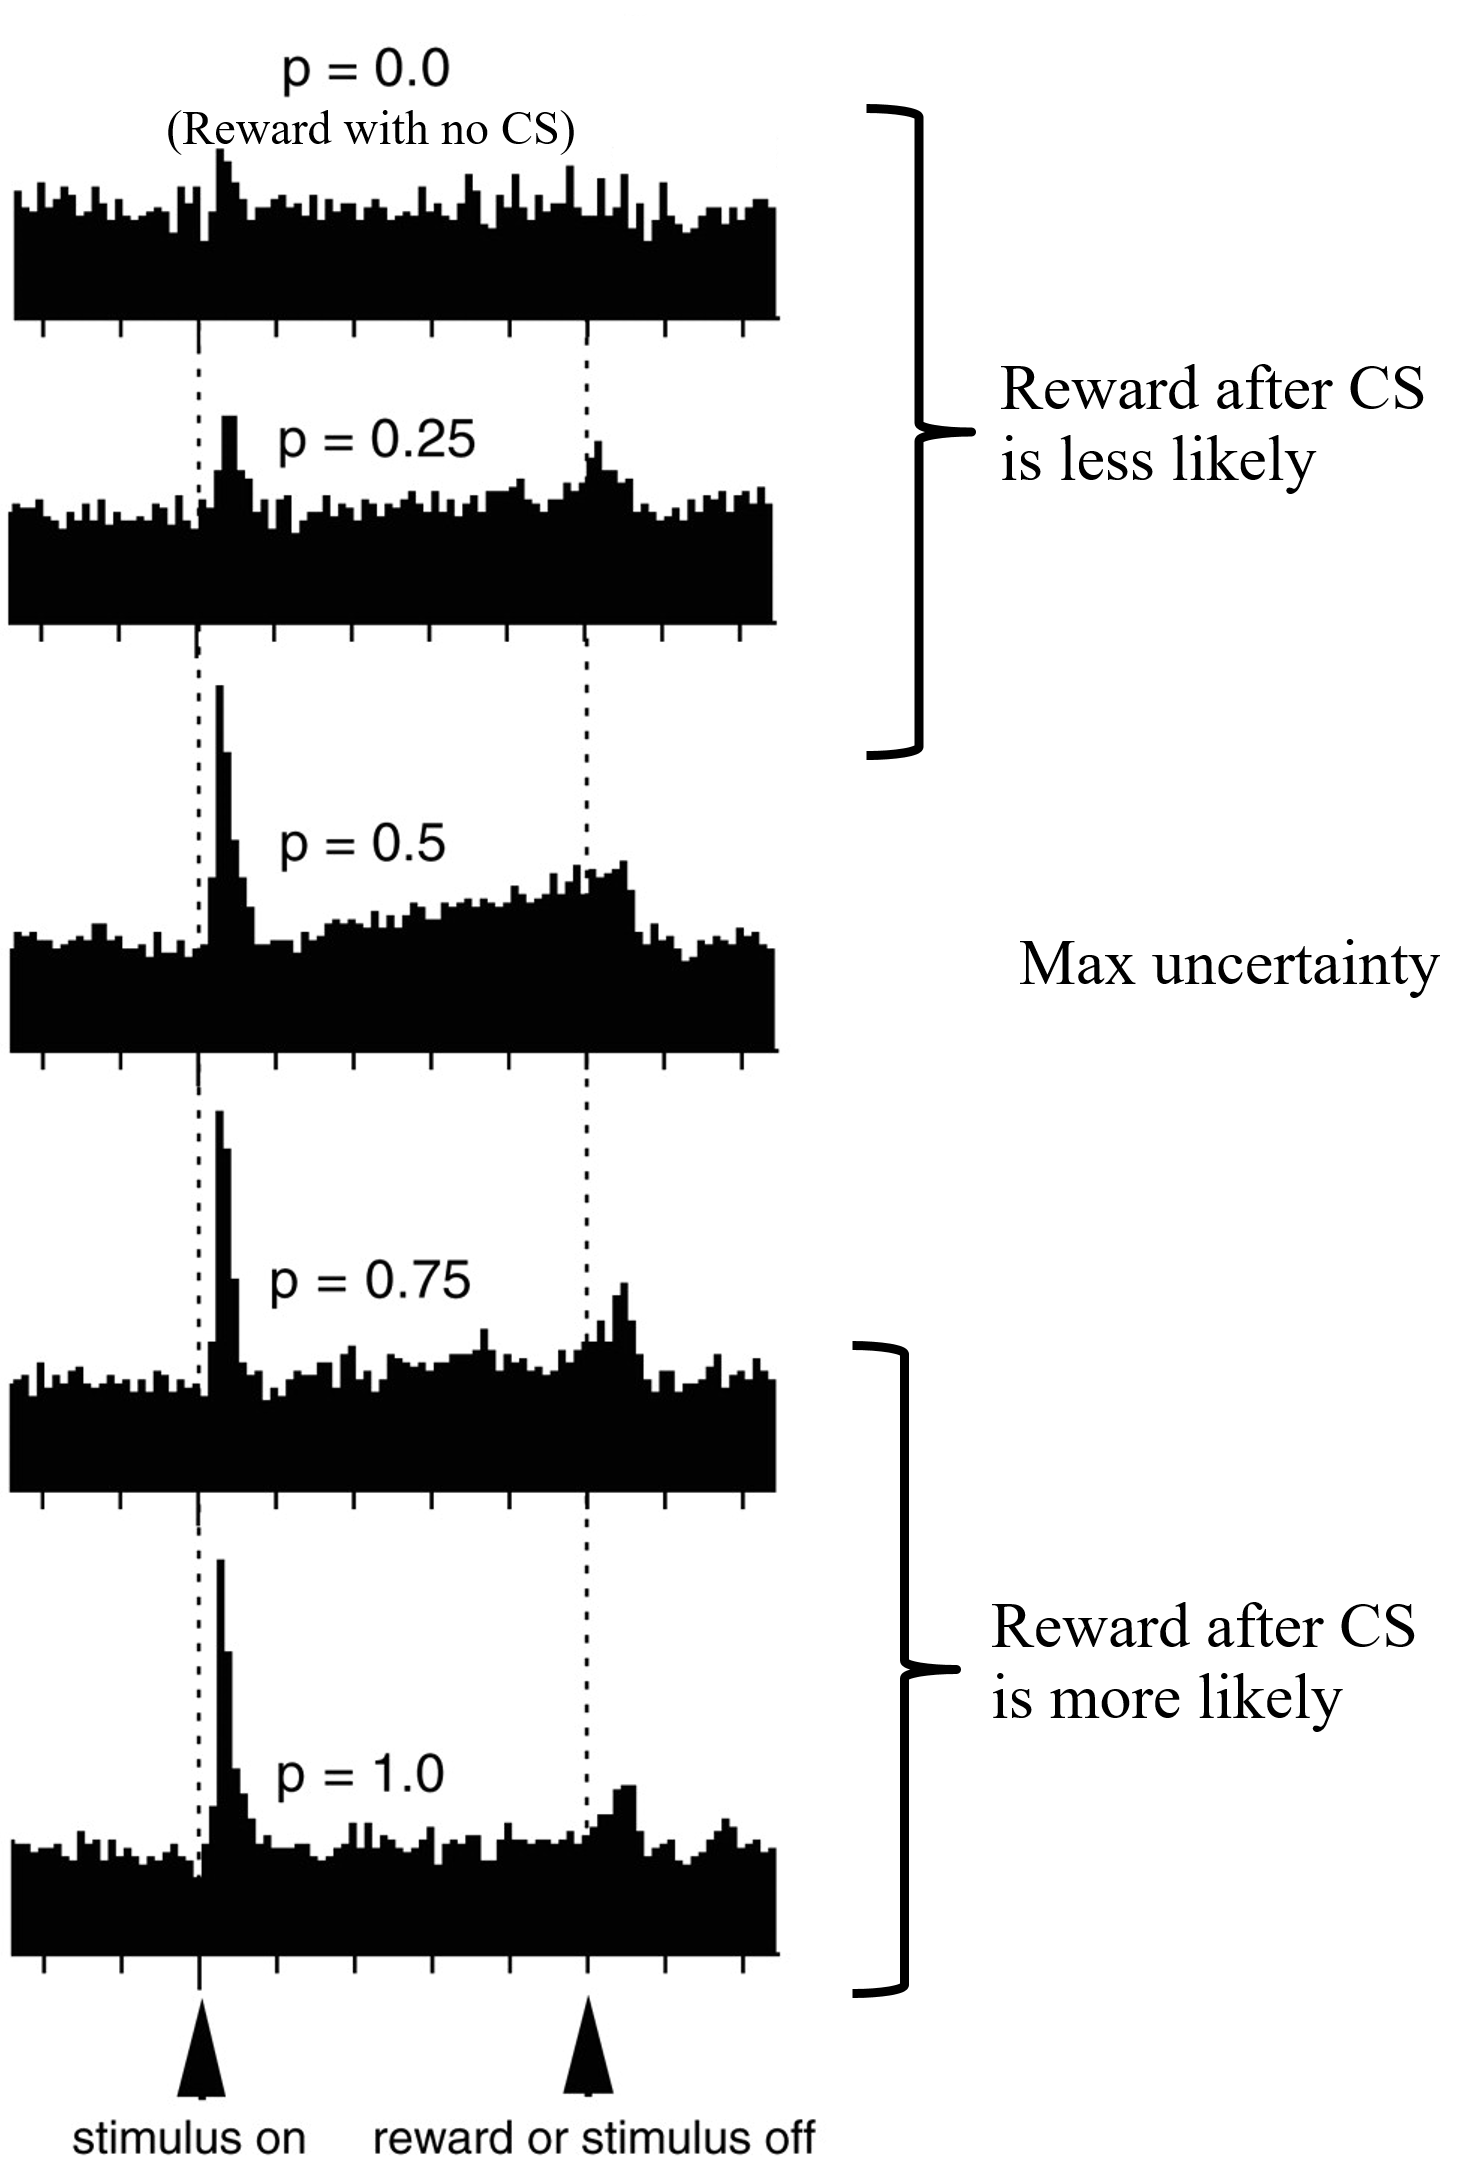
\includegraphics[width=0.65\linewidth]{./img/dopamine_probability.png}
        \end{center}

    \item[Timing encoding] \marginnote{Dopamine timing encoding}
        Dopamine response to unexpectedness also involves timing.
        A dopaminergic response occurs when a reward is given earlier or later than expected.

        \begin{casestudy}
            After learning that a reward occurs 1 second after the end of the \ac{cs}, 
            dopamine neurons fire if the timing changes.
            \begin{center}
                \includegraphics[width=0.5\linewidth]{./img/dopamine_timing.png}
            \end{center}
        \end{casestudy}
\end{description}

\begin{remark}
    Dopamine is therefore a signal for the predicted error and not strictly for the reward.
\end{remark}
    \chapter{Instrumental learning}


Form of control learning that aims to learn action-outcome associations:
\begin{itemize}
    \item When a reinforcer is likely to occur.
    \item Which actions bring to those reinforcers.
\end{itemize}
This allows the animal to act in anticipation of a reinforcer.

Instrumental learning includes:
\begin{descriptionlist}
    \item[Habitual system] \marginnote{Habitual system}
        Learn to repeat previously successful actions.
    \item[Goal-directed system] \marginnote{Goal-directed system}
        Evaluate actions based on their anticipated consequences.
\end{descriptionlist}

Depending on the outcome, the effect varies:
\begin{descriptionlist}
    \item[Positive reinforcement] \marginnote{Positive reinforcement}
        Delivering an appetitive outcome to an action increases the probability of emitting it.

    \item[Positive punishment] \marginnote{Positive punishment}
        Delivering an aversive outcome to an action decreases the probability of emitting it.
    
    \item[Negative reinforcement] \marginnote{Negative reinforcement}
        Omitting an aversive outcome to an action increases the probability of emitting it.
    
    \item[Negative punishment] \marginnote{Negative punishment}
        Omitting an appetitive outcome to an action decreases the probability of emitting it.
\end{descriptionlist}

\begin{table}[H]
    \centering
    \begin{tabular}{r|cc}
        \toprule
                            & \textbf{Delivery}                         & \textbf{Omission} \\
        \midrule
        \textbf{Appetitive} & Positive reinforcement (\texttt{+prob})   & Negative punishment (\texttt{-prob}) \\
        \textbf{Aversive}   & Positive punishment (\texttt{-prob})      & Negative reinforcement (\texttt{+prob}) \\
        \bottomrule
    \end{tabular}
    \caption{Summary of the possible effects}
\end{table}



\section{Types of schedule}

There are two types of learning:
\begin{descriptionlist}
    \item[Continuous schedule] \marginnote{Continuous schedule}
        The desired action is followed by the outcome every time.
        \begin{remark}
            More effective to teach a new association.
        \end{remark}

    \item[Partial schedule] \marginnote{Partial schedule}
        The desired action is not always followed by the outcome.
        \begin{remark}
            Learning is slower but the response is more resistant to extinction.
        \end{remark}

        There are four types of partial schedules:
        \begin{descriptionlist}
            \item[Fixed-ratio] 
                Outcome available after a specific number of responses.

                This results in a high and steady rate of response, with a brief pause after the outcome is delivered.


            \item[Variable-ratio] 
                Outcome available after an unpredictable number of responses.

                This results in a high and steady rate of response.


            \item[Fixed-interval] 
                Outcome available after a specific interval of time.

                This results in a high rate of response near the end of the interval and a slowdown after the outcome is delivered.


            \item[Variable-interval] 
                Outcome available after an unpredictable interval of time.

                This results in a slow and steady rate of response.
        \end{descriptionlist}
\end{descriptionlist}

\begin{minipage}{0.55\linewidth}
    \begin{casestudy}[Aplysia Californica]
        An Aplysia Californica will withdraw its gill upon stimulating the siphon.
        \begin{itemize}
            \item Repeated mild stimulations will induce a habituation of the reflex.
            \item Repeated intense stimulations will induce a sensitization of the reflex.
        \end{itemize}
    \end{casestudy}
\end{minipage}
\begin{minipage}{0.4\linewidth}
    \centering
    \includegraphics[width=0.9\linewidth]{./img/gill_habituation.png}
\end{minipage}



\section{Dopamine}

There is evidence that dopamine is involved in learning action-outcome associations.

\begin{description}
    \item[Striatal activity on unexpected events] \marginnote{Striatal activity on unexpected events}
        When an unexpected event happens, there is a change in the activity of the striatum.
        There is an increase in response when the feedback is positive and a decrease when negative.

        \begin{casestudy}[Microelectrodes in substantia nigra]
            \phantom{}\\
            \begin{minipage}{0.7\linewidth}
                The activity of the substantia nigra of patients with Parkinson's disease is measured during a probabilistic instrumental learning task.
                The task consists of repeatedly drawing a card from two decks, followed by positive or negative feedback depending on the deck.
            \end{minipage}
            \begin{minipage}{0.3\linewidth}
                \centering
                \includegraphics[width=0.95\linewidth]{./img/instrumental_dopamine_sn1.png}
            \end{minipage}

            The increase and decrease in striatal activity can be clearly seen when the feedback is unexpected.
            \begin{figure}[H]
                \centering
                \includegraphics[width=\linewidth]{./img/instrumental_dopamine_sn2.png}
            \end{figure}
        \end{casestudy}

    \item[Dopamine effect on behavior] \marginnote{Dopamine effect on behavior}
        The amount of dopamine changes the learning behavior:
        \begin{itemize}
            \item Low levels of dopamine cause an impairment in learning from positive feedback.
                This happens because positive prediction errors cannot occur.
            
            \item High levels of dopamine cause an impairment in learning from negative feedback.
                This happens because negative prediction errors cannot occur.
        \end{itemize}

        \begin{casestudy}[Probabilistic selection task]
            This instrumental learning task has two phases:
            \begin{descriptionlist}
                \item[Learning]
                    There are three pairs of stimuli (symbols) and, at each trial, a pair is presented to the participant who selects one.
                    For each pair, a symbol has a higher probability of providing positive feedback while the other is more likely to be negative.
                    Moreover, the probabilities are different among the three pairs.

                    \begin{center}
                        \includegraphics[width=0.55\linewidth]{./img/instrumental_dopamine_selection1.png}
                    \end{center}

                    Participants are required to learn by trial and error the stimulus in each pair that leads to a positive reward.
                    Note that learning could be accomplished by:
                    \begin{itemize}
                        \item Recognizing the more rewarding stimulus.
                        \item Recognizing the less rewarding stimulus.
                        \item Both.
                    \end{itemize}

                \item[Testing]
                    Aims to assess if participants learned to select positive feedback or avoid negative feedback.

                    The same task as above is repeated but all combinations of the stimuli among the three pairs are possible.
            \end{descriptionlist}

            Three groups of participants are considered for this experiment:
            \begin{enumerate}
                \item Those who took the cabergoline drug (dopamine antagonist).
                \item Those who took the haloperidol drug (dopamine agonist).
                \item Those who took a drug without effects (placebo).
            \end{enumerate}

            \begin{center}
                \includegraphics[width=0.55\linewidth]{./img/instrumental_dopamine_selection2.png}
            \end{center}

            Results show that:
            \begin{enumerate}
                \item Cabergoline inhibited positive feedback learning.
                \item Haloperidol enhanced positive feedback learning.
                \item Placebo learned positive and negative feedback equally.
            \end{enumerate}
        \end{casestudy}
        
        \begin{casestudy}
            It has been observed that:
            \begin{itemize}
                \item Reward prediction errors are correlated with activity in the left posterior putamen and left ventral striatum.
                \item Punishment prediction errors are correlated with activity in the right anterior insula.
            \end{itemize}

            \begin{center}
                \includegraphics[width=0.5\linewidth]{./img/pe_location.png}
            \end{center}
        \end{casestudy}

    \item[Actor-critic model] \marginnote{Actor-critic model}
        Model to correlate Pavlovian and instrumental learning. 
        It is composed by:
        \begin{itemize}
            \item The cortex is responsible for representing the current state.
            \item The basal ganglia implement two computational models:
                \begin{descriptionlist}
                    \item[Critic] \marginnote{Critic}
                        Learns stimulus-outcome associations and is active in both Pavlovian and instrumental learning.
                        It might be implemented in the ventral striatum, the amygdala and the orbitofrontal cortex.
                
                    \item[Actor] \marginnote{Actor}
                        Learns stimulus-action associations and is only active during instrumental learning.
                        It might be implemented in the dorsal striatum.
                \end{descriptionlist}
        \end{itemize}
\end{description}

\begin{casestudy}[Food and cocaine]
    \phantom{}
    \begin{itemize}
        \item Food-induced dopamine response is modulated by the reward expectations that promote learning until the prediction matches the actual outcome.
        \item Cocaine-induced dopamine response causes a continuous increase in the predicted reward that
            will eventually surpass all other cues and bias decision-making towards cocaine.
    \end{itemize}
    \begin{center}
        \includegraphics[width=0.8\linewidth]{./img/dopamine_food_cocaine.png}
    \end{center}
\end{casestudy}



\section{Learning strategies historical evolution}


% Instrumental learning can happen in two ways:
% \begin{descriptionlist}
%     \item[Cognitive map] \marginnote{Cognitive map}
%         Actions are taken based on the expected reward.
    
%     \item[Response strategy] \marginnote{Response strategy}
%         Actions are associated with particular stimuli.
% \end{descriptionlist}


\subsection{Generation 0}

There were two possible learning strategies:
\begin{descriptionlist}
    \item[Stimulus-response theory] \marginnote{Stimulus-response theory}
        Learning happens by creating stimulus-response associations.

        Learning does not happen if there is no reward.

    \item[Cognitive map / Field theory] \marginnote{Cognitive map / Field theory}
        A mental map is created and used to find the best action in a given state based on the expected reward.

        \begin{description}
            \item[Latent learning] \marginnote{Latent learning}
                Learning that is not shown behaviorally unless there is enough motivation.
        \end{description}
\end{descriptionlist}

\begin{casestudy}[Maze]
    An animal is put at the start of a maze where a reward is located in the west arm.
    After some training iterations, the animal is put at the other entrance:
    \begin{itemize}
        \item If it goes to the west arm, it learned to solve the maze using a cognitive map/place strategy.
        \item If it goes to the east arm, it learned to solve the maze using a stimulus-response strategy.
    \end{itemize}
    \begin{center}
        \includegraphics[width=0.55\linewidth]{./img/instrumental_maze.png}
    \end{center}

    It has been observed that rats start by learning a cognitive map (i.e. the environment is unknown).
    After enough training, they start relying on a response strategy (i.e. the environment is stable).
\end{casestudy}

\begin{casestudy}[Tolman's maze]
    Consider a maze with curtains and doors to prevent a long-distance perspective.
    \begin{center}
        \includegraphics[width=0.35\linewidth]{./img/tolman_maze.png}
    \end{center}

    Two groups of hungry rats have been considered to solve the maze:
    \begin{descriptionlist}
        \item[Group 1] No reward for solving the maze.
        \item[Group 2] Reward for solving the maze.
    \end{descriptionlist}
    It has been shown that the second group completes the maze faster.
    \begin{center}
        \includegraphics[width=0.45\linewidth]{./img/tolman_experiment1.png}
    \end{center}

    To show latent learning, three groups of hungry rats have been considered:
    \begin{descriptionlist}
        \item[Group 1] No reward for solving the maze.
        \item[Group 2] Reward for solving the maze.
        \item[Group 3] Reward for solving the maze starting from day 11.
    \end{descriptionlist}
    It has been shown that rats of the third group complete the maze faster as soon as they receive food.
    \begin{center}
        \includegraphics[width=0.45\linewidth]{./img/tolman_experiment2.png}
    \end{center}
\end{casestudy}


\subsection{Generation 1} 

Shifted from studying the spatial domain to a more general domain.
Based on two types of actions:
\begin{descriptionlist}
    \item[Goal-directed action] \marginnote{Goal-directed action}
        Actions made because a desired outcome is expected.
        An action is goal-directed if:
        \begin{itemize}
            \item There is knowledge of the relationship between action and consequences (response-outcome).
            \item The outcome is motivationally relevant.
        \end{itemize}

        Goal-directed behavior has the following properties:
        \begin{itemize}
            \item Involves active deliberation.
            \item Has a high computational cost.
            \item It is flexible to changes of the environmental contingency (i.e. stops if no reward occurs)
        \end{itemize}

        \begin{center}
            \includegraphics[width=0.65\linewidth]{./img/goal_directed_behavior.png}
        \end{center}

    \item[Habitual action] \marginnote{Habitual action}
        Actions made automatically just because they were rewarded in the past.
        They are not influenced by the current outcome even if it is undesired.

        Habitual behavior has the following properties:
        \begin{itemize}
            \item Does not require active deliberation.
            \item Has a low computational cost.
            \item It is inflexible to changes of the environmental contingency.
        \end{itemize}

        \begin{center}
            \includegraphics[width=0.65\linewidth]{./img/habitual_behavior.png}
        \end{center}

\end{descriptionlist} 

\begin{casestudy}[Goal-directed vs habitual behavior]
    The experiment is done in three steps:
    \begin{descriptionlist}
        \item[Training] 
            The animal undergoes instrumental learning (e.g. associate that by pressing a lever some food will be dropped).
        
        \item[Devaluation] 
            Manipulate the learned behavior by either:
            \begin{itemize}
                \item Devaluate the reinforcer.
                \item Degradate the contingency.
            \end{itemize}

        \item[Testing] 
            Repeat the training scenario without reward:
            \begin{itemize}
                \item If the action associated with a devaluated reinforcer is performed less, the behavior is goal-directed.
                \item If the frequency of the action is the same, the behavior is habitual.
            \end{itemize}
    \end{descriptionlist}

    \begin{remark}
        The training phase aims to instill a goal-directed behavior.
        On the other hand, if the animal is overtrained, it will learn a habitual behavior.
        The experiment can be done both ways.
    \end{remark}

    \begin{center}
        \includegraphics[width=0.85\linewidth]{./img/goal_directed_vs_habitual.png}
    \end{center}
\end{casestudy}

It has been hypothesized that the striatum might be the interface where rewards influence actions as: \marginnote{Striatum}
\begin{itemize}
    \item The basal ganglia are involved in the selection of actions.
    \item The SNc affects the plasticity of the striatum through the release of dopamine.
\end{itemize}

Moreover, different sections of the striatum are responsible for different types of behavior:
\begin{descriptionlist}
    \item[Dorsomedial striatum] Supports goal-directed behavior.
    \item[Dorsolateral striatum] Supports habitual behavior.
\end{descriptionlist}
This also hints that goal-directed and habitual behaviors act simultaneously and competitively (see \hyperref[sec:instrumental_gen3]{Generation 3}).


\subsection{Generation 2} 

Studied goal-directed and habitual behavior in humans.

\begin{description}
    \item[Functional magnetic resonance imaging (fRMI)] \marginnote{Functional magnetic resonance imaging (fRMI)}
        Measures the ratio of oxygenated to deoxygenated hemoglobin molecules in the brain.
        It allows to indirectly measure the neuronal activity of the brain on a high spatial resolution (i.e. allows to see where things happen but not when).
\end{description}

\begin{casestudy}[Goal-directed behavior in humans]
    Candidates are trained to select between two fractals of which 
    one leads to a reward with a high probability and the other with a low probability.
    The possible rewards are chocolate, tomato juice and orange juice (used as a control outcome).

    \begin{figure}[H]
        \centering
        \includegraphics[width=0.45\linewidth]{./img/human_goal_directed_experiment.png}
        \caption{
            Structure of the task. The high probability choice leads to the primary reward (chocolate or tomato juice) with probability $0.4$, 
            to the control reward (orange juice) with probability $0.3$ and to nothing with probability $0.3$.
            The low probability choice leads to the control reward with probability $0.3$ and nothing in the other cases.
            The neutral case leads to an empty glass or nothing.
        }
    \end{figure}

    After training, one of the primary rewards is devalued through selective satiation and the other is labeled as the valued outcome.
    Then, the training task is repeated.
    \begin{figure}[H]
        \centering
        \includegraphics[width=0.55\linewidth]{./img/human_goal_directed_experiment2.png}
        \caption{
            Steps of the experiment. In this figure, the devalued reward is the tomato juice.        
        }
    \end{figure}

    Behavioral results show that:
    \begin{itemize}
        \item During training, candidates favored the high-probability actions associated with chocolate and tomato juice.
            On the other hand, choices for the neutral condition were evenly distributed.
        \item The pleasantness rating for the devalued reward lowered after devaluation while the valued reward remained higher.
        \item During testing, candidates reduced their choice of the high-probability action associated with the devalued reward.
    \end{itemize}
    \begin{figure}[H]
        \centering
        \includegraphics[width=0.9\linewidth]{./img/human_goal_directed_experiment3.png}
    \end{figure}

    During both training and testing, the fRMIs of the candidates were taken.
    Neural results show that the \textbf{medial orbitofrontal cortex }has a significant modulation in its activity during instrumental action selection
    depending on the value of the associated outcome.
    \begin{figure}[H]
        \centering
        \includegraphics[width=0.4\linewidth]{./img/human_goal_directed_experiment4.png}
    \end{figure}
\end{casestudy}

\begin{casestudy}[Habitual behavior in humans]
    Candidates are presented, at each round of the trial, with a fractal image and a schematic indicating which button to press.
    The button can be pressed an arbitrary number of times and, at each press, on the screen appears:
    \begin{itemize}
        \item A gray circle (no reward).
        \item The image of an M\&M's {\tiny ©} or Frito {\tiny ©} (reward) with probability $0.1$. 
            To each fractal, only a type of reward can appear.
    \end{itemize} 
    \begin{figure}[H]
        \centering
        \includegraphics[width=0.6\linewidth]{./img/human_habitual_experiment.png}
    \end{figure}

    After training, one of the food rewards is devalued through selective satiation.
    Then, during testing, the same training task with the same stimulus-response-outcome is repeated without a reward.

    Two groups have been considered:
    \begin{descriptionlist}
        \item[1-day group] with little training.
        \item[3-day group] with extensive training.
    \end{descriptionlist}

    Behavioral results show that:
    \begin{itemize}
        \item Before devaluation, there were no significant differences between the responses of the two groups independently of the type of food.
        \item During testing, the 1-day group showed a goal-directed behavior while the 3-day group showed a habitual behavior.
    \end{itemize}
    \begin{figure}[H]
        \centering
        \includegraphics[width=0.55\linewidth]{./img/human_habitual_experiment2.png}
    \end{figure}

    During both training and testing, the fRMIs of the candidates were taken.
    Neural results show that, in the 3-day group, the \textbf{dorsolateral striatum} had significant activity.
\end{casestudy}


\subsection{Generation 3} \label{sec:instrumental_gen3}

Formalized goal-directed and habitual actions:

\begin{descriptionlist}
    \item[Model-based] (Goal-directed) \marginnote{Model-based}
        Use a model to predict the consequences of actions in terms of future states and expected rewards from future states.
    
        When the environment changes, the agent can update its policy of future states without the need to actually be in those states.

    \item[Model-free] (Habitual) \marginnote{Model-free}
        Select actions based on the stored state-action pairs learned over many trials.

        When the environment changes, the agent has to move into the new states and experience them.

    \item[Hybrid model] \marginnote{Hybrid model}
        Integrated computational and neural architecture where 
        model-based and model-free systems act simultaneously and competitively.

        This is the currently favored model for behavior.
\end{descriptionlist}


\begin{casestudy}[Latent learning in humans]
    The experiment consists of a sequential two-choice Markov decision task in which candidates navigate a binary decision tree.

    Each state contains a fractal image and
    candidates can choose to move to the left or right branch, each of which will lead with probability $0.7/0.3$ to one of the two subsequent states.
    When a leaf is reached, a monetary reward (0\textcentoldstyle, 10\textcentoldstyle\, or 25\textcentoldstyle) is delivered.
    \begin{figure}[H]
        \centering
        \includegraphics[width=0.4\linewidth]{./img/human_latent_experiment.png}
    \end{figure}

    \begin{minipage}{0.58\linewidth}
        The experiment is divided into two sessions:
        \begin{descriptionlist}
            \item[First session]
                Candidates choices are fixed but they can learn the transition probabilities.
    
            \item[Before second session]
                Candidates are presented with the association between fractal and reward.
    
            \item[Second session]
                Candidates are free to choose their actions at each state.
        \end{descriptionlist}
    \end{minipage}
    \begin{minipage}{0.4\linewidth}
        \centering
        \includegraphics[width=0.95\linewidth]{./img/human_latent_experiment2.png}
    \end{minipage}\\[1em]

    \begin{minipage}{0.7\linewidth}
        Behavioral results show that the majority of the candidates are able to make the optimal choice.
        This indicates that their behavior cannot be explained using a model-free learning theory (as learning only happens with a reward).
        A hybrid model has been proposed to model the candidates' behavior. It includes:
        \begin{descriptionlist}
            \item[Reward prediction error] Associated to model-free learning.
            \item[State prediction error] Associated to model-based learning.
        \end{descriptionlist}
    \end{minipage}
    \begin{minipage}{0.3\linewidth}
        \centering
        \includegraphics[width=\linewidth]{./img/human_latent_experiment3.png}
    \end{minipage}\\[1em]

    On a neuronal level, fRMIs show that:
    \begin{itemize}
        \item State prediction error activates the \textbf{intraparietal sulcus} and the \textbf{lateral prefrontal cortex}.
        \item Reward prediction error activates the \textbf{ventral striatum}.
    \end{itemize}
    \begin{figure}[H]
        \centering
        \includegraphics[width=0.75\linewidth]{./img/human_latent_experiment4.png}
    \end{figure}
\end{casestudy}

\begin{casestudy}[Model-free vs model-based in humans]
    Consider a Markov decision task that works as follows:
    \begin{itemize}
        \item In the first stage, candidates have to choose between two fractal images, 
            each leading to one of the two subsequent states with probability $0.7$ (common) and $0.3$ (rare).
        \item In the second stage, candidates have to choose between two fractal images, 
            each of which will lead to a monetary reward with a certain independent probability.
        \item The probability of receiving the reward changes stochastically during the trials.
    \end{itemize}
    \begin{figure}[H]
        \centering
        \includegraphics[width=0.35\linewidth]{./img/model_free_based_theoretical.png}
    \end{figure}

    It is expected that:
    \begin{descriptionlist}
        \item[Model-free agents] 
            Ignore the transition structure and prefer to repeat actions that lead to a reward in the past.

        \item[Model-based agents] 
            Respect the transition structure and modify their policies depending on the outcome.

            They are more likely to repeat an action following a rewarding trial only if that transition is common.
    \end{descriptionlist}

    Despite that, the actual results on human candidates show that a hybrid model is more suited to explain human behavior.
    \begin{figure}[H]
        \centering
        \includegraphics[width=0.6\linewidth]{./img/human_hybrid_model.png}
    \end{figure}

    % \begin{figure}[H]
    %     \centering
    %     \includegraphics[width=0.5\linewidth]{./img/model_free_based_theoretical2.png}
    % \end{figure}

    Neural results from fRMIs also show that the activity in the \textbf{striatum} increases for both model-based and model-free prediction errors.
\end{casestudy}

    \eoc
    
\end{document}